%!TEX program = pdflatex
%!BIB program = bibtex
\documentclass[journal]{IEEEtran}
\usepackage{graphicx}  % 用于 includegraphics
\usepackage{booktabs}  % 用于表格 midrule
\usepackage{subfigure}  % show sub-figure
\usepackage{algorithm}  % for algrithm
\usepackage{algorithmic}  % for algrithm
\usepackage{multirow}  % for multirow command used in the table
\usepackage{amsfonts}  % for mathbb
\usepackage{color,xcolor}  % 用于改变字体颜色
\usepackage{amssymb}  % 用于打对号
\usepackage{amsfonts}  % 用于 mathbb
\usepackage{url}  % 用于使用连接
\usepackage{ulem}  % 用于添加下划线
\usepackage{amsmath}
\newcommand{\eg}{e.g.}
\newcommand{\ie}{i.e.}
%\renewcommand{\uline}{}

% 题目
\hyphenation{op-tical net-works semi-conduc-tor}
\begin{document}
\title{A Simple and Strong Baseline for Universal Targeted Attacks on Siamese Visual Tracking}
\author{
  Zhenbang Li, Yaya Shi, Jin Gao, Shaoru Wang, Bing Li, Pengpeng Liang, Weiming Hu
  \thanks{This work is supported by the National Key R\&D Program of China (No. 2018AAA0102802), the Natural Science Foundation of China (Grant No. 62036011, 61721004), the Key Research Program of Frontier Sciences, CAS, Grant No. QYZDJ-SSW-JSC040. \textit{(Corresponding author: Jin Gao.)}}
  
  \thanks{Z. Li, J. Gao, S. Wang and B. Li are with the National Laboratory of Pattern Recognition, Institute of Automation, Chinese Academy of Sciences, Beijing, 100190, China, and also with School of Artificial Intelligence, University of Chinese Academy of Sciences, Beijing, 100190, China (e-mail: zhenbang.li@nlpr.ia.ac.cn; jin.gao@nlpr.ia.ac.cn; shaoru.wang@nlpr.ia.ac.cn; bli@nlpr.ia.ac.cn).}
  \thanks{Y. Shi is with the University of Science and Technology of China, Anhui, 230026, China (e-mail: shiyaya@mail.ustc.edu.cn).}
  \thanks{P. Liang is with Zhengzhou University, Henan, 450001, China (e-mail: liangpcs@gmail.com).}
  \thanks{W. Hu is with CAS Center for Excellence in Brain Science and Intelligence Technology, National Laboratory of Pattern Recognition, Institute of Automation, Chinese Academy of Sciences, Beijing, 100190, China, and also with School of Artificial Intelligence, University of Chinese Academy of Sciences, Beijing, 100190, China (e-mail: wmhu@nlpr.ia.ac.cn).}
}

\markboth{Journal of \LaTeX\ Class Files,~Vol.~14, No.~8, August~2015}
{Shell \MakeLowercase{\textit{et al.}}: Bare Demo of IEEEtran.cls for IEEE Journals}
\maketitle

% 摘要
\begin{abstract}
Siamese trackers are shown to be vulnerable to adversarial attacks recently. However, the existing attack methods craft the perturbations for each video independently, which comes at a non-negligible computational cost. In this paper, we show the existence of universal perturbations that can enable the targeted attack, e.g., forcing a tracker to follow the ground-truth trajectory with specified offsets, to be video-agnostic and free from inference in a network. 
%\uline{
Specifically, we attack a tracker by adding a universal translucent perturbation to the template image and adding a \textit{fake target},
%}
i.e., a small universal adversarial patch, into the search images adhering to the predefined trajectory, so that the tracker outputs the location and size of the \textit{fake target} instead of the real target. Our approach allows perturbing a novel video to come at no additional cost except the mere addition operations -- and not require gradient optimization or network inference. Experimental results on several datasets demonstrate that our approach can effectively fool the Siamese trackers in a targeted attack manner. 
We show that the proposed perturbations are not only universal across videos, but also generalize well across different trackers. Such perturbations are therefore doubly universal, both with respect to the data and the network architectures.
We will make our code publicly available.

\end{abstract}

% 关键字
\begin{IEEEkeywords}
Visual tracking, adversarial attacks, Siamese networks.
\end{IEEEkeywords}
\IEEEpeerreviewmaketitle

% 引言
\section{Introduction}
\IEEEPARstart{G}{iven} an arbitrary detected or annotated object of interest in the initial video frame, visual object tracking is aimed at {\it recognizing} and {\it localizing} other instances of the same object in subsequent frames. This paradigm of tracking visual objects from a single initial exemplar in the online-tracking phase has been broadly cast as a Siamese network-based one-shot problem recently \cite{DBLP:journals/tcsv/ShanZLZH21,DBLP:journals/tcsv/FanSZYL21,DBLP:journals/tcsv/LiPWK20,9258983}, which is termed as Siamese visual tracking and recognised as highly effective and efficient for visual tracking.

% \begin{figure}[t]
%   \centering
%   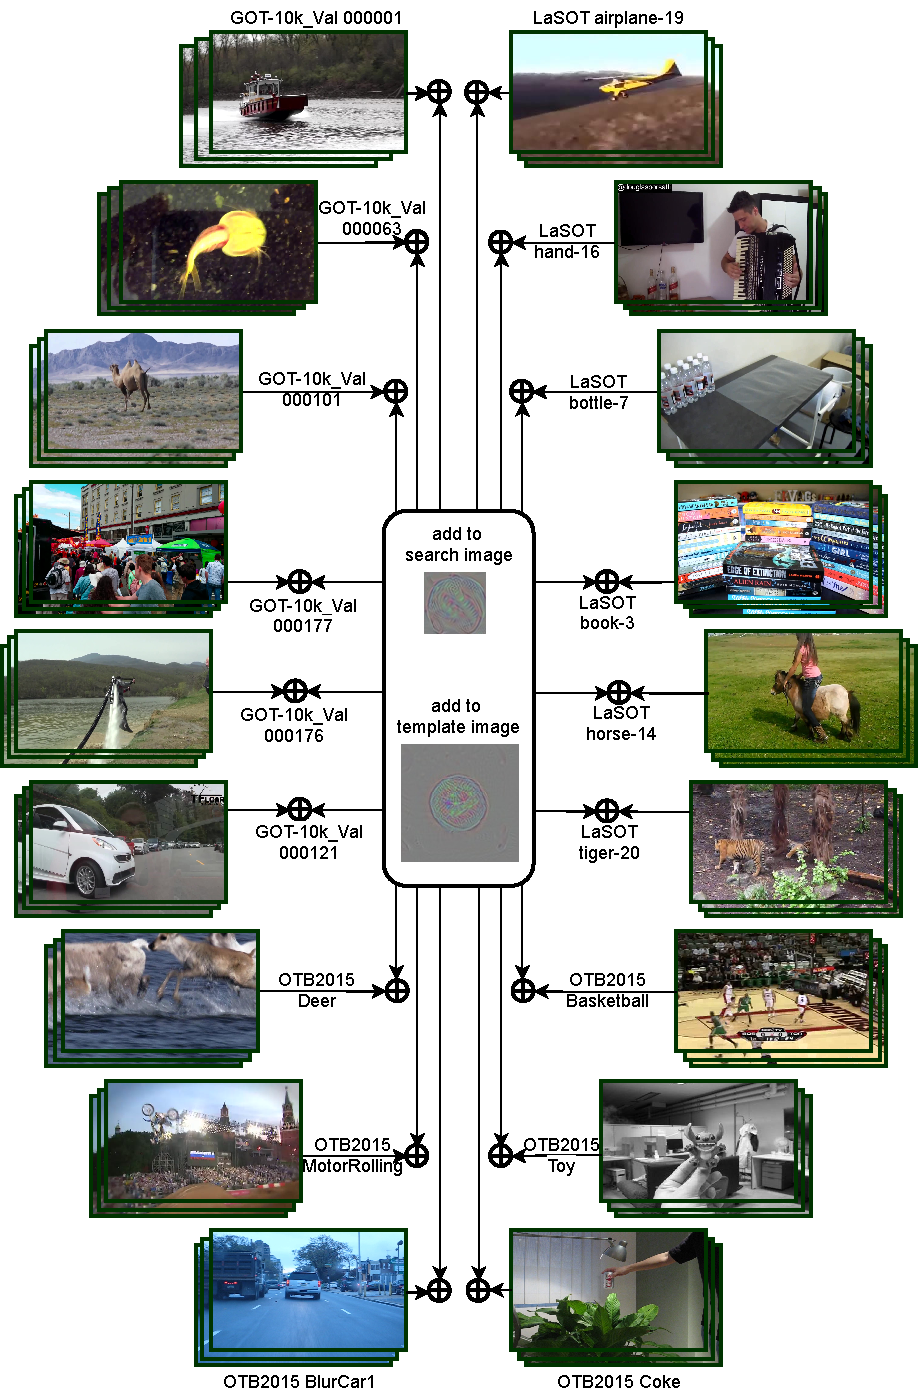
\includegraphics[width=0.48\textwidth]{images_imperceptible/UAP.pdf}
%   \caption{Being universal, the generated perturbations can be conveniently exploited to perturb videos on-the-fly without extra computations except the mere addition operations.} 
%   \label{fig:UAP}
% \end{figure}

\begin{figure}[t]
  \centering
  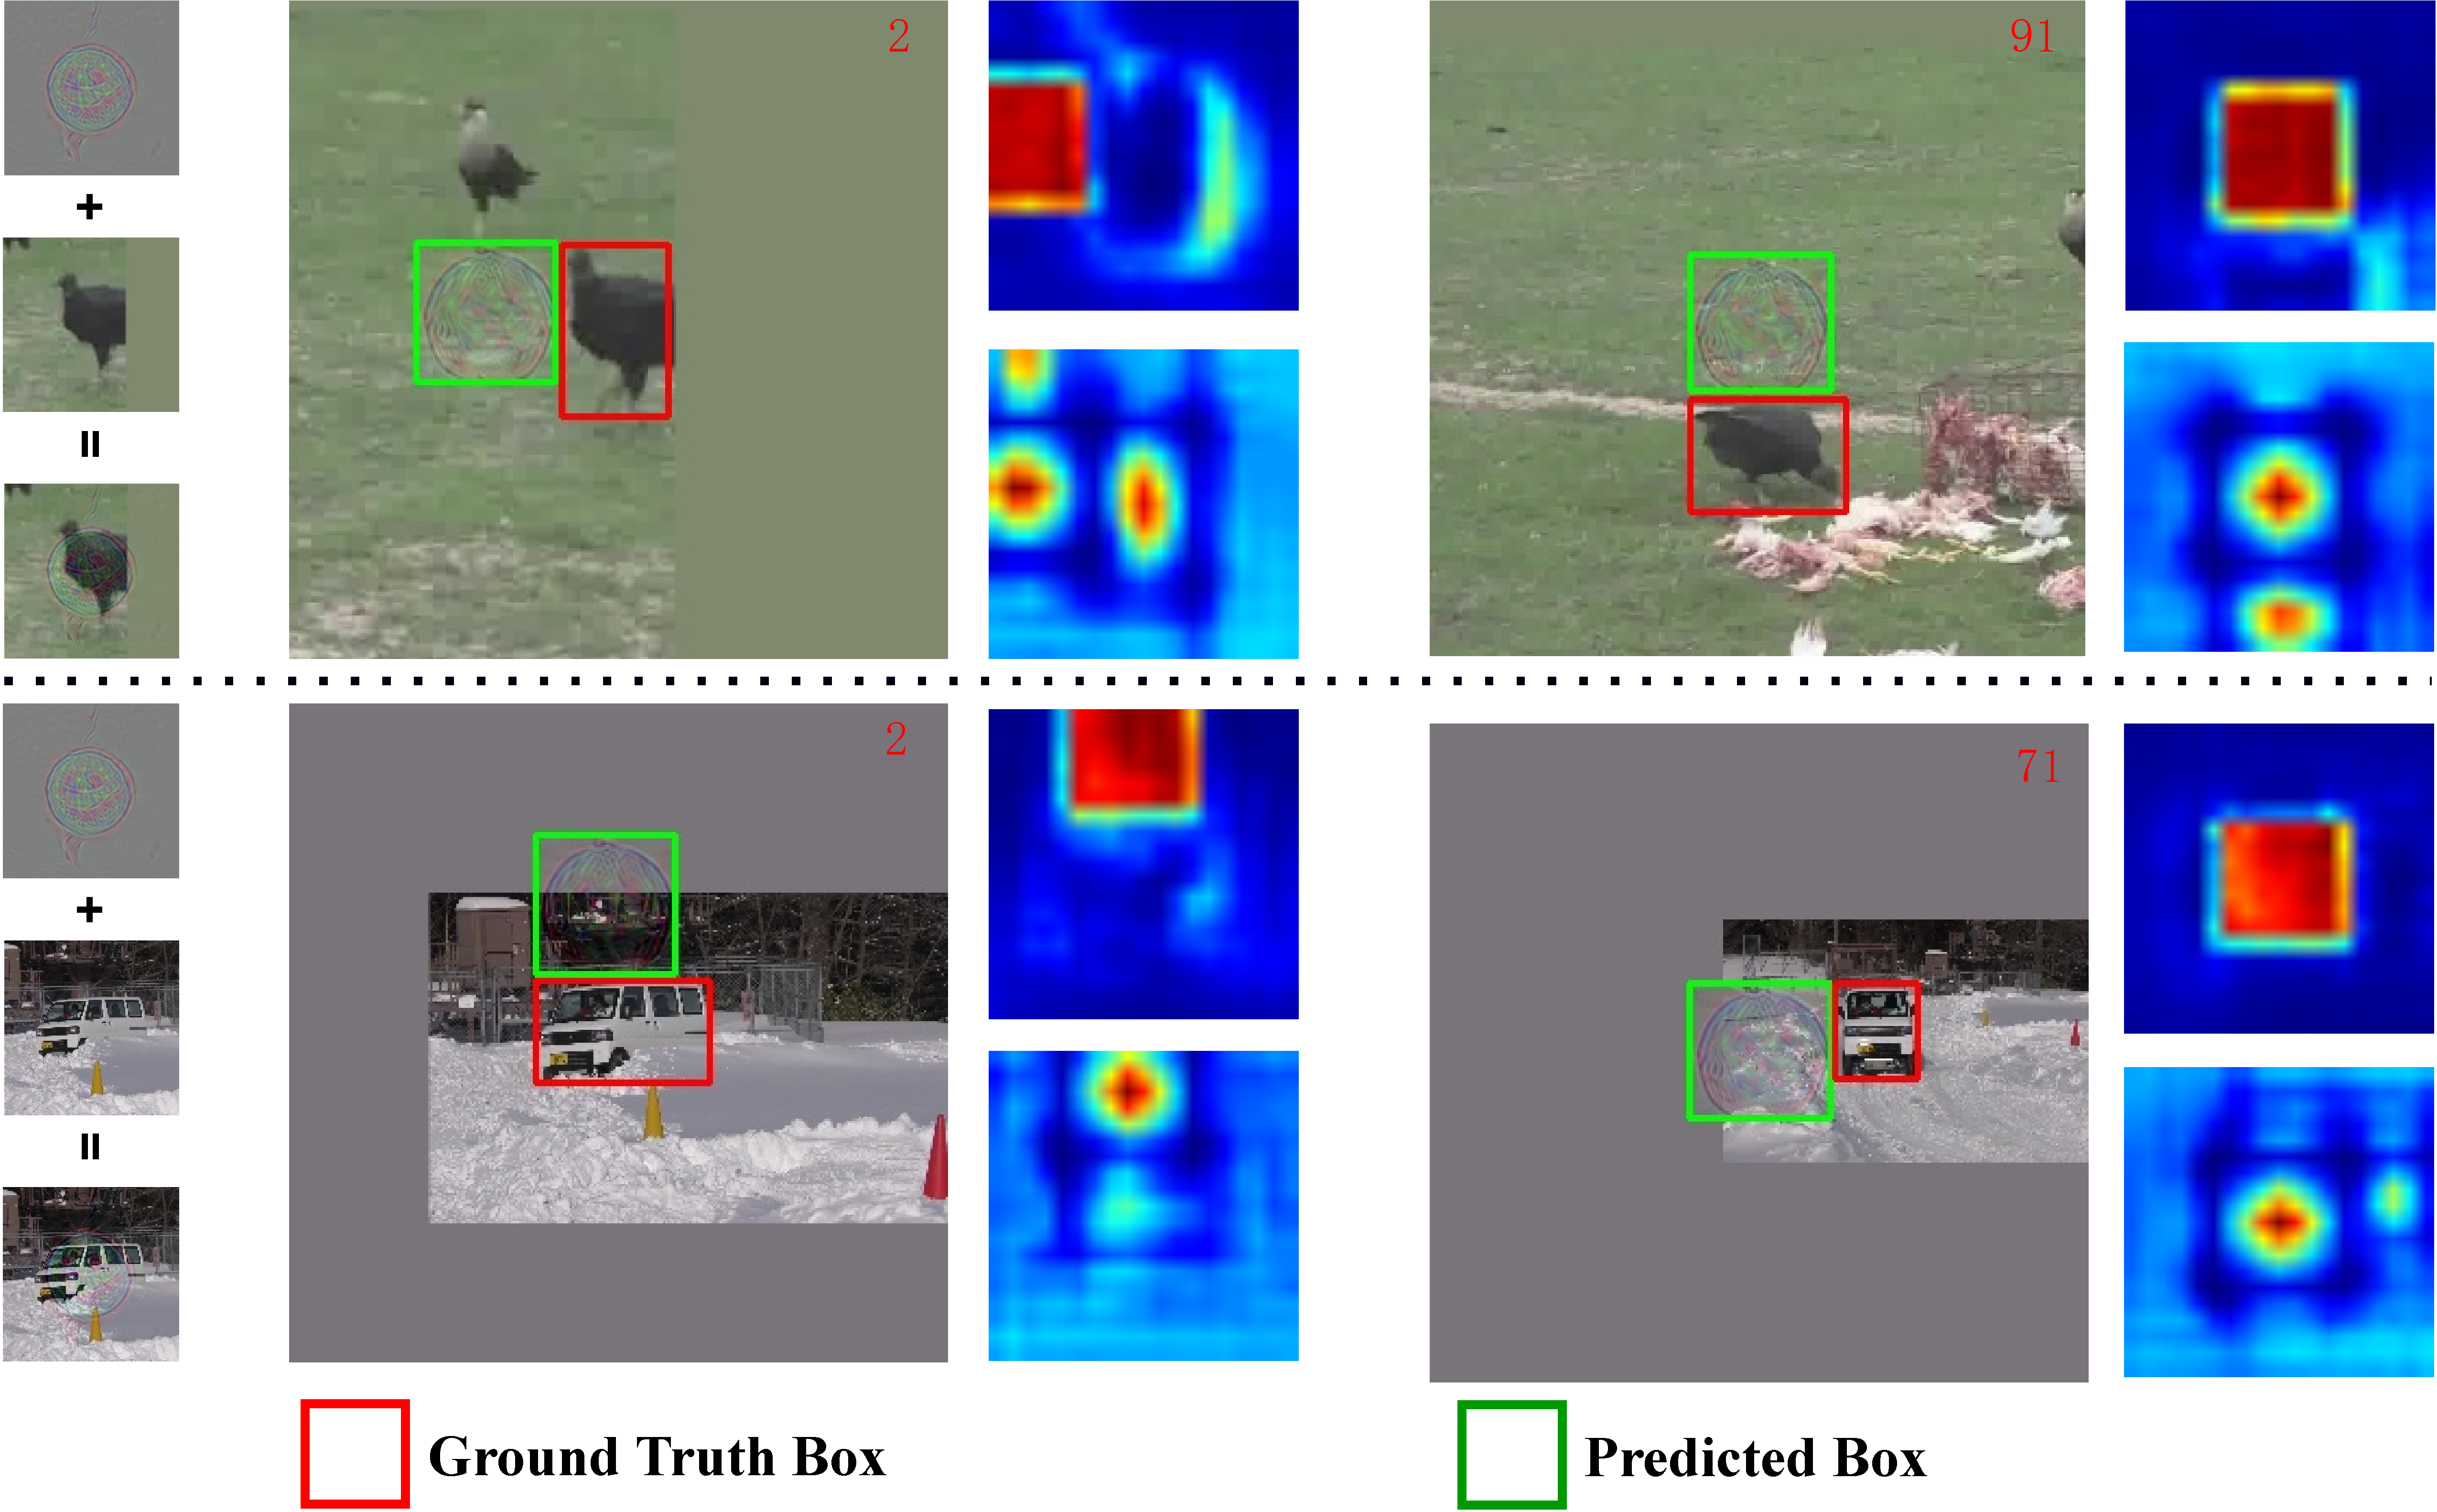
\includegraphics[width=0.485\textwidth]{images_imperceptible/1_v8.pdf}
  \caption{An illustration of our attacks to SiamFC++ on some example tracking sequences from GOT-10k benchmark. Our approach generates the video-agnostic perturbations which can force SiamFC++ to follow a complicated trajectory at virtually no cost. This is realized by off-line training the perturbations so that the tracker mistakenly believes the \textit{fake target} area contains the object to be tracked (see the top heatmap). Moreover, the quality assessment branch in SiamFC++ is also misled to confirm this result (see the bottom heatmap). The \textit{fake target} size is gradually decreased.} 
  %Being universal, the generated perturbations can be conveniently exploited to perturb videos on-the-fly without extra computations. 
  %Red represents the ground-truth bounding box, and green represents the predicted bounding box by the tracker.
  %The purple dashed box marks the universal adversarial patch. The left heatmap represents the probability of each spatial position to contain the \textit{fake target}, and the right heatmap represents the target state estimation quality.}
  \label{fig:1}
\end{figure}

Recently, the robustness of Siamese trackers has attracted much attention in the sense of testing their vulnerability to adversarial attacks, and the focus has been directed towards more efficient and low-cost attacks \cite{TTP,FAN,SPARK,chen2020one}. However, these attack methods still need to craft the perturbations for each video independently based on either iterative optimization or adversarial network inference, for which the adequacy of additional computational resources may be not ensured by the computationally intensive tracking systems. 

Universal adversarial perturbations (UAPs) proposed in \cite{UAP} can fool most images from a data distribution in an image-agnostic manner. Being universal, UAPs can be conveniently exploited to perturb unseen data on-the-fly without extra computations. However, no existing work has touched the topic of attacking the Siamese trackers using UAPs, because it is hard to apply existing UAPs to attack Siamese trackers directly. The main reason lies in the fact that, (a) most UAPs are designed for typical neural networks with one image as input while Siamese networks accept both the template and search images, and (b) the goal of existing UAP methods is to disturb unary or binary model outputs for single instance while we need to use universal perturbations to mislead Siamese trackers to follow a specified trajectory.
  
In this paper, we make the first attempt in finding the universal perturbations that fool a state-of-the-art Siamese tracker, \ie, SiamFC++ \cite{SiamFC++}, in a targeted attack manner, which comes at virtually no cost in the online-tracking phase. Specifically, we aim to attack the trackers by adding a universal perturbation to the template image and adding a \textit{fake target}, \ie, a small universal adversarial patch, into the search image adhering to the predefined trajectory (as shown in Figure \ref{fig:1}), so that the tracker outputs the location and size of the \textit{fake target} instead of the real target. Our generated video-agnostic perturbations allow perturbing a novel video to come at no additional cost except the mere addition operations -- and not require gradient optimization or network inference. Experiment results on OTB2015 \cite{OTB}, GOT-10k \cite{GOT-10k}, LaSOT \uline{\cite{LaSOT}}, UAV123 \cite{UAV123}, \uline{VOT2016} \cite{VOT2016}, VOT2018 \cite{VOT2018} and VOT2019 \cite{VOT2019} benchmarks demonstrate the effectiveness and efficiency of our approach.

% To sum up, the main contributions of this paper are:
% \begin{itemize}
%   \item To the best of our knowledge, we are the first to perform universal targeted attacks for Siamese trackers utilizing both the imperceptible perturbation and the adversarial patch together, which are jointly trained in an end-to-end manner.
%   \item We demonstrate that the adversarial patch can be rather small: the 32-by-32 patch can make the AO score drop dramatically to 0.146 and its area only accounts for 1\% of the search image area.
%   \item Although trained using the parameters of the SiamFC++ \cite{SiamFC++} network, the universal perturbations can perform black box attacks on other trackers such as SiamRPN \cite{SiamRPN} and SiamRPN++ \cite{SiamRPN++}.
% \end{itemize}

\section{Related Work}

\subsection{Siamese Visual Tracking}

Siamese visual tracking is a fundamental research direction in template matching-based tracking besides the correlation filter-based methods. Both of them are aimed to ``causally'' estimate the positions of a template cropped from the initial video frame in the subsequent frames.
%\uline{A comprehensive survey of the related trackers is beyond the scope of this paper, so we only briefly review two aspects that are most relevant to our work. Please refer to \cite{9339950} for a thorough survey on visual object tracking methods.} 
\uline{
% 4 高晋1 2021 是一个相关滤波算法
Liu et. al. \cite{9376997} propose a correlation filtering tracking algorithm based on the visual memory multi-template update strategy.
% 5 高晋2 2021 是一个相关滤波算法
Liu et. al. \cite{9132673} construct a fuzzy aided detection module to boost the correlation filtering tracking system.
}
Siamese trackers formulate visual tracking as learning cross-correlation similarities between a target template and the candidates in the search region in a convolution fashion. Tracking is then performed by locating the object in the search image region based on the highest visual similarity. This paradigm is formulated as a local one-shot detection task.

Recently, some Siamese trackers~\cite{SiamFC++,SiamRPN,SiamRPN++} have demonstrated a significant performance improvement in visual tracking. 
In particular, SiamRPN \cite{SiamRPN} consists of one Siamese subnetwork for feature extraction and another region proposal subnetwork including the classification and regression branches separately. Based on its success in the decomposition of classification and state estimation, SiamRPN++ \cite{SiamRPN++} further breaks the restriction of strict translation invariance through a simple yet effective spatial aware sampling strategy and successfully trains a ResNet-driven Siamese tracker with significant performance gains. Apart from these anchor-based methods, an anchor-free tracker SiamFC++ \cite{SiamFC++} is further designed by considering non-ambiguous scoring, prior target scale/ratio distribution, knowledge-free and estimation quality assessment guidelines.
\uline{
% Ocean
Ocean \cite{zhang2020ocean} directly predicts the position and scale of target objects in an anchor-free fashion. Since each pixel in groundtruth boxes is well trained, the tracker is capable of rectifying inexact predictions of target objects during inference.
% FCOT
FCOT \cite{cui2020fully} introduces an online regression model generator (RMG) based on the carefully designed anchor-free box regression branch, which enables the tracker to be more effective in handling target deformation during tracking procedure.
%  SiamCAR
SiamCAR \cite{9157720} is both proposal and anchor free, and decomposes tracking into two subproblems: one classification problem and one regression task. SiamCAR takes one unique response map to predict object location and bounding box directly.
}
In our experiments, we are focused on the anchor-free SiamFC++ tracker, whereas the transferability of our generated adversarial attacks to the previous anchor-based trackers is also studied.
\uline{
A comprehensive survey of the related trackers is beyond the scope of this paper, please refer to \cite{9339950} for a thorough survey on visual object tracking methods.} 

\subsection{Adversarial Attacks}

Adversarial attacks \cite{9169672} to image classification were first investigated in \cite{intriguing} with the aim of identifying the vulnerability of modern deep networks to imperceptible perturbations. 
Recent studies also emerge to investigate the adversarial attacks to other diverse types of tasks such as natural language processing \cite{generating,zhang2020adversarial,morris2020textattack,jin2020bert} and object detection \cite{wei2019transferable}.
\uline{
Research topics related to adversarial attacks includes digital watermarking \cite{9343885}, 3D face presentation attacks \cite{9294085} and adversarial defense \cite{9169672}.
Xiong et. al. \cite{9343885} propose to generate the digital watermarking by slightly modifying the pixel values of video frames to protect video content from unauthorized access. Compared with \cite{9343885}, our purpose of modifying pixel values of video frames is attacking the tracker, instead of detecting the illegal distribution of a digital movie.
Jia et. al. \cite{9294085} propose to generate 3D face artifacts to attack the face recognition network. Compared with \cite{9294085}, our method directly modifies the input of the network instead of changing the input of cameras using 3D face artifacts.
Wang et. al. \cite{9169672} propose the white-box attack/defense methods for image classifiers. Compared with \cite{9169672}, we focus on attacking the object tracking networks instead of the image classification networks.
}

Scenarios of possible adversarial attacks can be categorized along different dimensions.

\textit{White box attacks v.s. Black box attacks} In the white box attack setting \cite{meng2019white}, the adversary has full knowledge of the model including model type, model architecture and values of all parameters and trainable weights. In the black box setting \cite{cheng2018query,li2019nattack,papernot2017practical,li2020projection}, the adversary has limited or no knowledge about the model under attack \cite{kurakin2018adversarial}. In this paper, we focus on the white box attack for Siamese trackers. However, although we train perturbations using the parameters of the SiamFC++ \cite{SiamFC++} network, we surprisingly find that the trained perturbations can perform black box attacks on other trackers such as SiamRPN \cite{SiamRPN} and SiamRPN++ \cite{SiamRPN++}.

\textit{Non-universal attacks v.s. Universal attacks} In the setting of non-universal attacks \cite{dai2018adversarial,li2018second,lin2017tactics}, the adversary has to generate one perturbation for every new datapoint, which is time consuming. In the setting of the universal attacks \cite{khrulkov2018art,mopuri2018nag,zhang2020understanding,mopuri2018generalizable,chen2018shapeshifter}, only one perturbation is generated and used for every datapoint of the dataset. In this paper, we focus on generating universal perturbations for Siamese trackers to perform efficient attacks.
\iffalse
\begin{figure}[t]
  \centering
  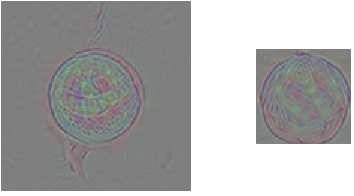
\includegraphics[width=0.35\textwidth]{images_imperceptible/vis_perturbations.pdf}
  \caption{Visualization of the generated perturbations. Left: The template perturbation. Right: The adversarial patch.}
  \label{fig:vis_perturbations}
\end{figure}
\fi

\iffalse
\textit{Optimization based attacks and GAN based attacks}
The optimization based attacks are slow and can only optimize perturbation for one specific instance each time.
To avoid this, the GAN based methods use GAN to generate perturbation for one datapoint without loop. 
However, the GAN networks run for every datapoint, which occupies the GPU memory and time. 
In this paper, we generate perturbations in an offline manner, which do not require gradient optimization or network inference.
\fi

\textit{Imperceptible Perturbations v.s. Adversarial Patch} The imperceptible perturbations most commonly modify each pixel by a small amount and can be found using a number of optimization strategies such as Limited-memory BFGS \cite{intriguing} and PGD \cite{PGD}.
Different from the imperceptible perturbations, the adversarial patch is extremely salient to a neural network. The adversarial patch can be placed anywhere into the input image to cause the network to misbehave, and thus is commonly used for universal attacks \cite{patch}.
% To the best of our knowledge, we are the first to attack object trackers utilizing both the imperceptible perturbation and the adversarial patch together, which are jointly trained in an end-to-end manner.
Note that our adversarial patch works in the image domain instead of the network domain. In the network-domain case, the noise is allowed to take any value and is not restricted to the dynamic range of image value as in the image-domain case \cite{karmon2018lavan}.

\textit{Untargeted Attacks v.s. Targeted Attacks} In the case of untargeted attacks, the adversary's goal is to cause the network to predict any incorrect label and whatever the incorrect label is does not matter, \eg, pushing the object location estimation just outside the true search region in visual tracking.
Targeted attacks, however, aim to change the network's prediction to some specific target label. In visual tracking, the targeted attacks aim to intentionally drive trackers to output specified object locations following a predefined trajectory.

\subsection{Adversarial Attacks in Visual Tracking}

Recently, there are several explorations of the adversarial attacks to the visual tracking task. For example, PAT \cite{PAT} generates physical adversarial textures via white-box attacks to steer the tracker to lock on the texture when a tracked object moves in front of it. However, PAT validates its method by attacking a light deep regression tracker GOTURN \cite{GOTURN}, which has low tracking accuracy on modern benchmarks. In this paper, we aim to attack state-of-the-art Siamese trackers.
RTAA \cite{RTAA} takes temporal motion into consideration when generating lightweight perturbations over the estimated tracking results frame-by-frame. However, RTAA only performs the untargeted attacks for trackers, which is less challenging than the targeted attacks in this paper, as we aim to create arbitrary, complex trajectories at test time. 

Targeted attacks to follow an erroneous path which looks realistic are crucial to deceive the tracking system without raising any suspicion in the real-world applications.
%\uline{
SPARK \cite{SPARK} computes incremental perturbations by using information from the past frames to perform targeted attacks on Siamese trackers. 
%}
However, SPARK needs to generate distinct adversarial examples for every search image through heavy iterative schemes, which is time-consuming to attack online-tracking in real time. The recent real-time attacker in \cite{TTP} exclusively uses the template image to generate temporally-transferable perturbation in a one-shot manner, and then adds it to every search image. However, this method still needs to generate perturbations for each individual video, and its targeted attack setting requires diverse perturbations from several runs of network inference. It is ill-suited to attack a real-world online-tracking system when we can not get access to the limited computational resources. In this paper, however, we propose video-agnostic perturbations which allow perturbing a novel video to come at no additional cost except the mere addition operations.

% 方法
\section{Method}

\begin{figure}[t]
  \centering
  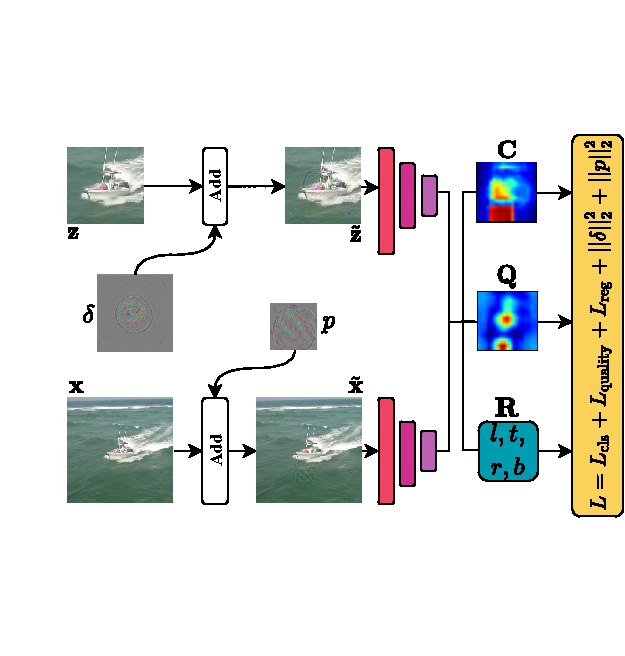
\includegraphics[width=0.49\textwidth]{images_imperceptible/network_v5.pdf}
  \caption{The training pipeline of the proposed method. We aim to train an imperceptible perturbation $\delta$ for the template image $\textbf z$, and an adversarial patch $p$ for the search image $\textbf x$. After adding $\delta$ to $\textbf z$ and adding the \textit{fake target} $p$ into $\textbf x$, the tracker outputs the location and size of the \textit{fake target} instead of the real target.}
  \label{fig:net}
\end{figure}

In this section, we introduce our video-agnostic targeted attack framework for Siamese trackers. We aim to attack the tracker by adding a perturbation to the template image and adding a \textit{fake target}, i.e., an adversarial patch, into the search images adhering to the predefined trajectory, so that the tracker outputs the location and size of the \textit{fake target} instead of the real target. Below, we formalize our targeted attacks to SiamFC++ \cite{SiamFC++}, and then introduce our perturbation strategy in detail.
 
\subsection{Problem Definition}

Let $V=\{I_i\}_1^T$ denote the frames of a video sequence of length $T$. $B^{gt}=\{b^{gt}_i\}_1^T$ is used to represent the target's ground-truth position in each frame. The visual object tracking aims to predict the position $B^{pred}=\{b^{pred}_i\}_1^T$ of this target in the subsequent frames given its initial state. In SiamFC++, the tracker first transforms the paired reference frame $I_1$ and annotation $b_1^{gt}$ to get \uline{a} template image $\textbf z_1$, and transforms the search frame $I_i$ to get the search image $\textbf x_i$ centered at the position estimated in the previous frame. At each time-step, the template image $\textbf z_1$ and the search image $\textbf x_i$ are first passed individually through a shared backbone network and then fused using a channel-wise correlation operation:
\begin{equation}
  \text{Feat}_{j}(\mathbf{z}_1, \mathbf{x}_i)=\psi_{j}(\phi(\mathbf{z}_1)) \star \psi_{j}(\phi(\mathbf{x}_i)), j \in\{\mathrm{cls}, \mathrm{reg}\}
\end{equation}
where $\star$ denotes the channel-wise correlation operation, $\phi(\cdot)$ denotes the feature extractor of the Siamese network, $\psi_j(\cdot)$ denotes the layers specific to the classification or regression task, and $j$ denotes the specific task type ($\mathrm{cls}$ denotes the classification task and $\mathrm{reg}$ denotes the regression task). $\psi_{\mathrm{cls}}$ and $\psi_{\mathrm{reg}}$ are both designed as two convolutional layers for adapting generic features to the feature space specific to the classification/regression task. The fused features then act as input to a head network, which predicts a classification map $\textbf{C}$, a bounding box regression map $\textbf{R}$, and a quality assessment map $\textbf{Q}$ in an anchor-free manner. In short, $\textbf C$ encodes the probability of each spatial position to contain the target, $\textbf R$ regresses the bounding box of the target, and $\textbf Q$ predicts the target state estimation quality. The final bounding box is then generated according to $\textbf{C}$, $\textbf{R}$ and $\textbf{Q}$.

A straight forward way to achieve targeted attacks for Siamese trackers is directly using popular attack methods such as FGSM \cite{FGSM} and BIM \cite{DBLP:conf/iclr/KurakinGB17a}:

\begin{equation}
\begin{gathered}
  \min\limits_{\delta_{\textbf{x}_{i}}, \delta_{\textbf{z}_{i}}} L(y^{fake}_i, f(\textbf{x}_i + \delta_{\textbf{x}_{i}}, \textbf{z}_i + \delta_{\textbf{z}_{i}}))\\
  \text{s.t.}\ ||\delta_{\textbf{x}_i}||_p \le \epsilon_1, ||\delta_{\textbf{z}_i}||_p \le \epsilon_2,
\end{gathered}
\end{equation}
where $L$ is the loss function of the SiamFC++ tracker. $(\textbf{x}_i, \textbf{z}_i)$ is the search-template pair of the video being tracked at frame $i$ and $\textbf{z}_i \equiv \textbf{z}_1$. $y^{fake}_i=\{\textbf{C}^*, \textbf{R}^*, \textbf{Q}^*\}$ is the fake target of the loss function generated according to the fake ground truth box $b^{fake}_i$ that we want the tracker to output at frame $i$ (see Sec. \ref{generate}). 
% 不写 BIM,原因是BIM的优化为 xi+1 = xi + delta, 与上面公式不太好兼容。
Additionally, $\delta$ should be sufficiently small, which is commonly modeled through an upper-bound $\epsilon$ on the $l_p\text{-norm}$, commonly denoted as $||\cdot||_p$, of the perturbation. A popular choice is to set $p=\infty$.
However, these methods require perturbing the input image pair $(\textbf{x}, \textbf{z})$ frame by frame, which comes at a non-negligible cost, considering that visual object tracking is a real-time task.
As a consequence, universal adversarial perturbations \cite{UAP, shafahi2020universal} are more practical for attacking Siamese trackers:
\begin{equation}
  \begin{gathered}
    \min\limits_{\delta_\textbf{x}, \delta_\textbf{z}} \mathop{\mathbb{E}}\limits_{(\textbf{x}, \textbf{z})} L(y^{fake}, f(\textbf{x} + \delta_\textbf{x}, \textbf{z} + \delta_\textbf{z}))\\
    \text{s.t.}\ ||\delta_\textbf{x}||_p \le \epsilon_1, ||\delta_\textbf{z}||_p \le \epsilon_2,
  \end{gathered}
\end{equation}  
where the input pair $(\textbf x,\textbf z)$ is randomly picked from the training set. 
Note that universal adversarial perterbations are added to the whole image and $y^{fake}$ is kept constant during the training process.
As shown in \cite{hirano2020simple}, this vanilla UAP method is limited to untargeted attacks.
To achieve universal targeted attacks, one feasible way is to paste a small (universal) adversarial patch into the search images adhering to the predefined trajectory, so that the tracker outputs the location and size of the adversarial patch instead of the real target:
\begin{equation}
    \min\limits_{\delta_\textbf{x}} \mathop{\mathbb{E}}\limits_{(\textbf{x}, \textbf{z}, y^{fake})} L(y^{fake}, f(A_{\text{paste}}(\textbf{x}, p_\textbf{x}, b^{fake}_{\textbf{x}}), \textbf{z})),
\end{equation}
%where $m$ is a binary mask and $m_{x,y}=1$ at all spatial locations under the fake ground bounding box $b^{fake}$ which is variable during training according to the patch position.
% $\odot$ is element-wise multiplication. 
where $A_{\text{paste}}$ is a patch application operator \cite{patch} which pastes the adversarial patch $p_\textbf{x}$ into the search image according to $b^{fake}_{\textbf{x}}$. Both $b^{fake}_{\textbf{x}}$ and $y^{fake}$ are variable during training.
\uline{$A_{paste}$ means that, in the region where the perturbation is pasted, the pixel values of the original image are replaced with the pixel values of the perturbation.}
Note that this vanilla adversarial patch method uses the clean template image during training. However, CNN attacks are usually expected \uline{imperceptibly} but the above method has to paste an obviously noticeable fake target patch to tracking frames, which raises the risk of being suspected.

%\uline{
To overcome all the shortcomings of the above methods, we propose to train a translucent perturbation $\delta$ for the template image $\textbf z$, and a translucent patch $p$ for the search image $\textbf x$. 
%}
After adding $\delta$ to $\textbf z$ and adding the fake target $p$ into $\textbf x$, the tracker outputs the location and size of the adversarial patch instead of the real target (see Figure \ref{fig:net}). Both $\delta$ and $p$ are universal (\ie, video-agnostic), which means perturbing a novel video only involves the mere addition of the perturbations to the template and search images -- and does not require gradient optimization or network inference.
\begin{equation}
  \begin{gathered}
    \min\limits_{\delta_\textbf{x}, \delta_\textbf{z}} \mathop{\mathbb{E}}\limits_{(\textbf{x}, \textbf{z}, y^{fake})} L(y^{fake}, f(A_{\text{add}}(\textbf{x}, p_\textbf{x}, b^{fake}_{\textbf{x}}), \textbf{z} + \delta_\textbf{z}))\\
    \text{s.t.}\ ||\delta_\textbf{x}||_p \le \epsilon_1, ||\delta_\textbf{z}||_p \le \epsilon_2,
  \end{gathered}
\end{equation}
where $A_{\text{add}}$ is a patch application operator which adds the patch into the search image according to $b^{fake}_{\textbf{x}}$.
\uline{$b^{fake} = \{x_0, y_0, x_1, y_1\}$ denotes the coordinates of the upper-left and lower-right corners of the fake target on the search image.}
\uline{The operator $A_{add}$ refers to the injection of small additive noise into the image. The injected noises are small and sometimes invisible to human eyes.}

Our attacks on Siamese visual tracking with both the template and search images as input, enable us to exploit both the perturbation generation method \cite{FGSM} and adversarial patch generation method \cite{patch} simultaneously. However, applying both of the above methods to trackers is non-trivial. In this paper, we demonstrate that the perturbations and the adversarial patch are both indispensable for attacking trackers and can be jointly optimized in an end-to-end training manner. On the one hand, the small patch applied to the search image works as a fake target. It is crucial to design a strategy for the tracker to follow a predefined trajectory. For example, the TTP method \cite{TTP} pre-computes perturbations corresponding to diverse directions and uses them to force the tracker to follow the target trajectory. However, this method is sub-optimal because the tracker only predicts the approximation of the specified trajectory. As shown in experiments, the targeted attack performance of TTP is not as good as ours.
\uline{On the other hand, the adversarial patch is usually added to the background region of the search image and does not change the pixel values in the foreground region where the real target exists. Therefore if we do not add the perturbation to the template image, the response values of the region where the real target exists on the heatmaps are always high. Thus it is necessary to perturb the template image to cooling down hot regions where the real target exists on the heatmaps and increasing the responses at the position of the fake target. (see Figure \ref{fig:1}).}

\begin{algorithm}[tb]
  \caption{Training Process}
  \label{alg:algorithm}
  \textbf{Input}: Training dataset $\mathcal{V}$, Siamese tracker $f$, and max iteration number $N$.\\
  \textbf{Output}: Translucent perturbation $\delta$, and adversarial patch $p$.
  \begin{algorithmic}[1] %[1] enables line numbers
  \STATE Let $k = 0$.
  \WHILE{$k < N$}
  \STATE Randomly pick a video $V\in \mathcal{V}$. The corresponding ground truth is $B^{gt}=\{b^{gt}_i\}^T_1$.
  \STATE Randomly pick paired frames $I_t, I_s$ from $V$.
  \STATE Generate template image $\textbf{z}$ according to $I_t$ and $b^{gt}_t$.
  \STATE $\tilde{\textbf{z}} = \textbf{z} + \delta_k.$
  \STATE Generate search image $\textbf{x}$ according to $I_s$ and $b^{gt}_s$.
  \STATE Calculate the \textit{fake target} position $\{x_0, y_0, x_1, y_1\}$ with respect to the search image.
  \STATE $\tilde{\textbf x} = A_{\text{add}}(\textbf x, p_k, \{x_0, y_0, x_1, y_1\}).$
  \STATE $\textbf{C, R, Q} = f(\tilde {\textbf x}, \tilde{\textbf z}).$
  \STATE Generate fake labels $\textbf{C}^*,\textbf{R}^*,\textbf{Q}^*$ using $\{x_0, y_0, x_1, y_1\}$.
  \STATE Calculate loss $L(\textbf{C, R, Q}, \textbf{C}^*, \textbf{R}^*, \textbf{Q}^*)$ using Equ. \ref{eq:loss}.
  \STATE $\delta_{k+1} = \delta_{k} - \epsilon_1 \cdot \text{sign}(\nabla_{\delta_k}L).$
  \STATE $p_{k+1} = p_{k} - \epsilon_2 \cdot \text{sign}(\nabla_{p_k}L).$
  \STATE $k = k + 1.$
  \ENDWHILE
  \STATE \textbf{return} $\delta_N, p_N.$
  \end{algorithmic}
  \label{alg}
\end{algorithm}

\begin{figure}[t]
  \centering
  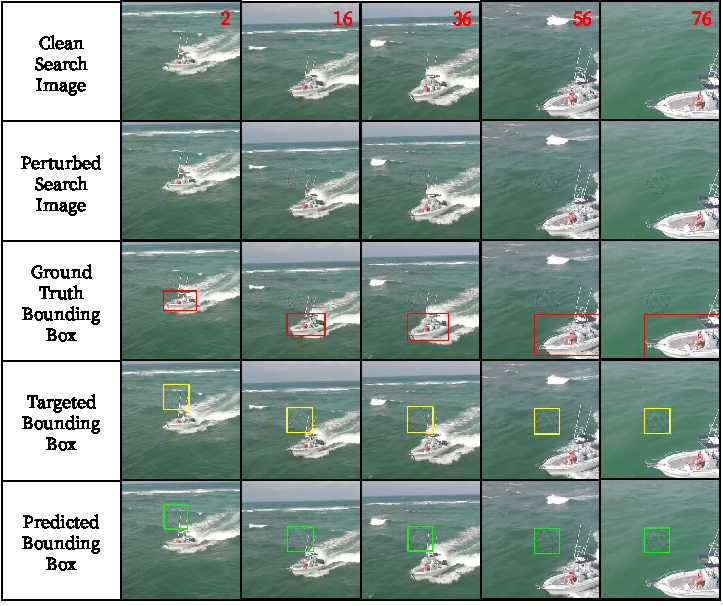
\includegraphics[width=0.49\textwidth]{images_imperceptible/vis_v7.pdf}
  \caption{Results of targeted attacks where the tracker is forced to follow a predefined \textit{fake trajectory} $B^{fake}=\{b^{fake}_i\}_1^{T}$ (indicated by the yellow bounding box). The \textit{fake trajectory} follows the \textit{real trajectory} $B^{gt}=\{b^{gt}_i\}_1^T$ (indicated by the red bounding box) and the adjacent boundaries of $b^{fake}_i$ and $b^{gt}_i$ are 2 pixels apart.}
  \label{fig:vis1}
\end{figure}

\subsection{Generating Video-Agnostic Perturbations}\label{generate}

In this subsection, we show how to train the video-agnostic perturbations $(\delta, p)$ for Siamese trackers. At beginning, each element in $\delta$ and $p$ is initialized to 0.
During the $k$-th iteration of training, a video $V=\{I_i\}_1^T$ is randomly selected from the training dataset $\mathcal V$. 
Assuming the template perturbation at the $k$-th iteration is $\delta_k \in \mathbb{R}^{127\times 127 \times 3}$, and the adversarial patch is $p_k$. 
We first randomly pick paired frames $I_t, I_s$ from $V$. The clean template image $\textbf z\in \mathbb{R}^{127\times 127 \times 3}$ is generated according to $I_t$ and $b^{gt}_t$, and the perturbed template image is:
\begin{equation}
\tilde {\textbf z} = \textbf z + \delta_k.
\end{equation}
Similarly, the clean search image $\textbf x \in \mathbb{R}^{303\times 303 \times 3}$ is generated according to $I_s$ and $b^{gt}_s$.
As mentioned before, the patch is regarded as a \textit{fake target} and added into the search images. We force the center position of the \textit{fake target} to near the center position of the real target within a shift range of 64 pixels, where the shift is defined as the maximum range of translation generated from a uniform distribution.
The perturbed search image is generated as follows:
\begin{equation}
\tilde{\textbf x} = A_{\text{add}}(\textbf x, p_k, \{x_0, y_0, x_1, y_1\}),
\end{equation}
where $ b^{fake} = \{x_0, y_0, x_1, y_1\}$ denotes the coordinates of the upper-left and lower-right corners of the fake target on the search image. 
\uline{$A_{add}$} adds the patch into the search image $\textbf x$ at location $(\frac{x_0+x_1}{2},\frac{y_0+y_1}{2})$. Subsequently, the SiamFC++ tracker takes $\tilde {\textbf x}$ and $\tilde{\textbf z}$ as input and predicts $\textbf{C, R, Q}$ in an anchor-free manner.

\textit{Generating Fake Labels} The fake lables are composed of three parts: fake classification label $\textbf{C}^*$, fake regression label $\textbf{R}^*$ and fake quality estimation label $\textbf{Q}^*$.

For classification, location $(x,y)$ on feature map $\psi_{\mathrm{cls}}$ is considered as a positive sample (i.e., $\textbf{C}^*_{x,y} = 1$) if its corresponding location $\left(\left\lfloor\frac{s}{2}\right\rfloor+x s,\left\lfloor\frac{s}{2}\right\rfloor+y s\right)$ on the input image falls into the fake bounding box, and vice versa are considered as negative samples (i.e., $\textbf{C}^*_{x,y} = 0$). $s=8$ denotes the total step length of the feature extraction network.

In the regression branch, the last convolution layer predicts the distance of position $\left(\left\lfloor\frac{s}{2}\right\rfloor+x s,\left\lfloor\frac{s}{2}\right\rfloor+y s\right)$ to the four edges of the fake ground truth bounding box, denoted as the four-dimensional vector $\boldsymbol{t}^{*}=\left(l^{*}, t^{*}, r^{*}, b^{*}\right)$. Thus, the fake regression label $\textbf{R}^*$ at position $(x,y)$ can be expressed as:

\begin{equation}
  \begin{array}{ll}
  l^{*}=\left(\left\lfloor\frac{s}{2}\right\rfloor+x s\right)-x_{0}, \quad t^{*}=\left(\left\lfloor\frac{s}{2}\right\rfloor+y s\right)-y_{0} \\
  r^{*}=x_{1}-\left(\left\lfloor\frac{s}{2}\right\rfloor+x s\right), \quad b^{*}=y_{1}-\left(\left\lfloor\frac{s}{2}\right\rfloor+y s\right)
  \end{array}
\end{equation}

SiamFC++ assumes that feature pixels near the center of the target will have higher importance than other pixels. Following the design of SiamFC++, we use a $1 \times 1$ convolutional layer for quality assessment, i.e., to learn the intersection over union (IoU) score of the predicted box $b^{pred}$ and $b^{fake}$:

\begin{equation}
  \mathrm{IoU}^{*}=\frac{\operatorname{ Intersection }\left(b^{pred}, b^{fake}\right)}{\operatorname{Union}\left(b^{pred}, b^{fake}\right)}
\end{equation}

\textit{Training Objective} The loss function is calculated as follows:
\begin{equation}
\begin{array}{l}
\begin{aligned}
L&=\frac{\alpha}{N_{\mathrm{pos}}} \sum_{x, y} L_{\mathrm{cls}}\left(\textbf{C}_{x, y}, \textbf{C}_{x, y}^{*}\right) \\
&+\frac{\beta}{N_{\mathrm{pos}}} \sum_{x, y} \textbf{1}_{\left\{\textbf{C}_{x, y}^{*}>0\right\}} L_{\mathrm{quality}}\left(\textbf{Q}_{x, y}, \textbf{Q}_{x, y}^{*}\right) \\
&+\frac{\gamma}{N_{\mathrm{pos}}} \sum_{x, y} \textbf{1}_{\left\{\textbf{C}_{x, y}^{*}>0\right\}} L_{\mathrm{reg}}\left(\textbf{R}_{x, y}, \textbf{R}_{x, y}^{*}\right) \\
&+\eta \cdot ||\delta_k||_2^2 +  \sigma \cdot ||p_k||^2_2,
\end{aligned}
\end{array}
\label{eq:loss}
\end{equation}
where $\textbf{C}_{x, y}, \textbf{R}_{x, y}, \textbf{Q}_{x, y}$ represent the values of $\textbf{C}, \textbf{R}, \textbf{Q}$ at location $(x, y)$, respectively. $\textbf{C}^*, \textbf{R}^*, \textbf{Q}^*$ are the fake labels generated according to the position and size of the \textit{fake target}. $\textbf 1$ is the indicator function that takes 1 if the condition in subscribe holds and takes 0 if not, $N_{\mathrm{pos}}$ denotes the number of positive samples in the training phase, $L_{\mathrm{cls}}$ denotes the focal loss \cite{focal} for classification result.
\iffalse
\begin{equation}
  \mathrm{FL}\left(p_{\mathrm{t}}\right)=-\alpha_{\mathrm{t}}\left(1-p_{\mathrm{t}}\right)^{\gamma} \log \left(p_{\mathrm{t}}\right)
\end{equation}
\fi
$L_{\mathrm{quality}}$ denotes the binary cross entropy (BCE) loss for quality assessment,
\iffalse
\begin{equation}
\begin{array}{ll}
\ell(x, y)=L=\left\{l_{1}, \ldots, l_{N}\right\}^{\top},\\
l_{n}=-w_{n}\left[y_{n} \cdot \log x_{n}+\left(1-y_{n}\right) \cdot \log \left(1-x_{n}\right)\right]
\end{array}
\end{equation}
\fi
and $L_{\mathrm{reg}}$ denotes the IoU loss \cite{iou-loss} for bounding box regression.
\iffalse
\begin{equation}
G I o U=I o U-\frac{|C \backslash(A \cup B)|}{|C|}
\end{equation}
\fi
%Following SiamFC++, we assign 1 to $\textbf{C}_{x, y}^{*}$ if $(x, y)$ is considered as a positive sample, and 0 if as a negative sample.
  
\textit{Optimization}
\uline{Before introducing the perturbation update process in offline training, we first revisit the popular adversarial example generation methods. One of the simplest methods to generate adversarial images $I^{adv}$ works by linearizing loss function in $L_{\infty}$ neighbourhood of a clean image and finds exact maximum of linearized function using following closed-form equation \cite{FGSM}:}
\begin{equation}
    I^{adv} = I + \epsilon \cdot \text{ sign} \bigl( \nabla_I L(I, y_{true})  \bigr),
    \vspace{-0.1cm}
\end{equation}
\uline{where $I$ is the input image, and the values of the pixels are integer numbers in the range [0, 255]. $y_{true}$ is the true label for the image $I$. $L(I, y)$ is the cost function of the neural network for the attack purpose, given image $I$ and label $y$. $\epsilon$ is a hyper-parameter to be chosen. A straightforward way to extend the above method is applying it multiple times with small step size. This leads to the Basic Iterative Method (BIM) introduced in \cite{DBLP:conf/iclr/KurakinGB17a}:}
\begin{equation}
    \begin{gathered}
        I_0^{adv} = I, \\
        I_{N+1}^{adv} = I_N^{adv}+\epsilon \cdot \text{ sign}(\nabla_I L(I_N^{adv},y_{true})),
    \end{gathered}
\end{equation}
%\uline{where $Clip_{I, \epsilon} \left\{ I' \right\}$ is the function which performs per-pixel clipping of the image $I'$, so that the result will be in $L_{\infty}$ $\epsilon$-neighbourhood of the source image $I$.}
\uline{The BIM can be easily made into an attacker for a specific desired target class, called the Iterative Target Class Method \cite{DBLP:conf/iclr/KurakinGB17a}:}
\begin{equation}
  \begin{gathered}
      I_0^{adv} = I,\\
      I_{N+1}^{adv} = I_N^{adv}-\epsilon \cdot \text{ sign}(\nabla_I L(I_N^{adv},y_{target})).
  \end{gathered}
  \label{equ:itcm}
\end{equation}

\uline{We utilize the Iterative Target Class Method to update the perturbation values during the training process.}
At each training step, the perturbations are updated as follows:
\begin{gather}
\delta_{k+1} = \delta_{k} - \epsilon_1 \cdot \text{sign}(\nabla_{\delta_k}L)\\
p_{k+1} = p_{k} - \epsilon_2 \cdot \text{sign}(\nabla_{p_k}L),
\end{gather}
where $\epsilon_1$ and $\epsilon_2$ are used to ensure that the perturbation added to the template/search image is small.
During training, we only optimize the values of perturbations $(\delta, p)$ and the parameters of the Siamese network remain intact. We outline this training procedure in Algorithm \ref{alg}.

\subsection{Attacking the Tracker at Inference Time}

Once the perturbations $(\delta, p)$ are trained, we can use them to perturb the template image and search images of any novel video for attacking. Both $\delta$ and $p$ are universal (i.e., video-agnostic), which means perturbing a novel video only involves the mere addition of the perturbations to the template and search images -- and does not require gradient optimization or network inference.
Assume $B^{fake}=\{b^{fake}_i\}_1^{T}$ is the trajectory we hope the tracker to output.
During tracking the $i$-th frame of the video $V=\{I_i\}_1^T$, we need to add $p$ into $\textbf x_i$ according to $b^{fake}_i=\{x_{0_i}, y_{0_i}, x_{1_i}, y_{1_i}\}$:
\begin{equation}
\tilde{\textbf x}_i = A_{\text{add}}(\textbf x_i, p, \{x_{0_i}, y_{0_i}, x_{1_i}, y_{1_i}\}).
\end{equation}
The tracker then takes $\tilde{\textbf z}_1=\textbf z_1+\delta$ and $\tilde{ \textbf x}_i$ as input, and the subsequent tracking procedure remains the same as SiamFC++.
We outline this procedure in Algorithm \ref{alg:algorithm_attack}.

\begin{table*}[t]
  \centering
  \caption{Characteristics of the datasets used to train and evaluate the proposed attack method.}
  \begin{tabular}{lrccccc} \toprule
  \multicolumn{2}{c}{Dataset}                            & Videos & Total frames & Frame rate & Object classes & Num. of attributes \\ \midrule
  \multirow{4}{*}{Training set} & GOT-10k training split & 9.34K  & 1.4M        & 10 fps     & 480            & 6                  \\
                                & LaSOT training split   & 1.12K  & 2.83M        & 30 fps     & 70             & 14                 \\
                                & COCO2017               & n/a    & 118K         & n/a        & 80             & n/a                \\
                                & ILSVRC-VID             & 5.4K   & 1.6M         & 30 fps     & 30             & n/a                \\ \midrule
  \multirow{7}{*}{Test set}     & GOT-10k validation split& 180   & 21K          & 10 fps     & 150            & 6                  \\
                                & UAV123                 & 123    & 113K         & 30 fps     & 9              & 12                 \\
                                & LaSOT test split       & 280    & 690K         & 30 fps     & 70             & 14                 \\
                                & OTB-15                 & 100    & 59K          & 30 fps     & 22             & 11                 \\
                                & VOT2016                & 60     & 21K          & 30 fps     & 16             & 6                  \\
                                & VOT2018                & 60     & 21K          & 30 fps     & 24             & 6                  \\ 
                                & VOT2019                & 60     & 19K          & 30 fps     & 30             & 6                  \\ \bottomrule
  \end{tabular}
  \label{tab:dataset}
\end{table*}

\begin{algorithm}[tb]
  \caption{Attack Process}
  \label{alg:algorithm_attack}
  \textbf{Input}: The trained perturbations $\delta$ and $p$, Siamese tracker $f$, video $V=\{I_i\}_1^T$. $b^{gt}_1$ is the position of the real target in the first frame. $B^{fake}=\{b^{fake}_i\}_1^{T}$ is the trajectory we hope the tracker to output.\\
  \textbf{Output}: $B^{pred}=\{b^{pred}_i\}_1^{T}$
  \begin{algorithmic}[1] %[1] enables line numbers
    \STATE Generate the clean template image $\textbf{z}_1$ according to $I_1$ and $b^{gt}_1$.
    \STATE Generate the perturbed template image $\tilde{\textbf z}_1=\textbf z_1+\delta$.
    \STATE Let $i = 2$.
  \WHILE{$i \le T$}
  \STATE Generate clean search image $\textbf{x}_i$ according to $I_i$ and $b^{pred}_{i-1}$.
  \STATE $b^{fake}_i=\{x_{0_i}, y_{0_i}, x_{1_i}, y_{1_i}\}$
  \STATE Generate the perturbed search image $\tilde{\textbf x}_i = A_{\text{add}}(\textbf x_i, p, \{x_{0_i}, y_{0_i}, x_{1_i}, y_{1_i}\}).$
  \STATE $\textbf{C, R, Q} = f(\tilde {\textbf x}_i, \tilde{\textbf z}_1).$
  \STATE Generate the predicted bounding box $b^{pred}_i$ according to $\textbf{C, R, Q}$.
  \STATE $i = i + 1.$
  \ENDWHILE
  \STATE \textbf{return} $B^{pred}$
  \end{algorithmic}
\end{algorithm}

% 实验
\section{Experiments}

\subsection{Experimental Setup}

\textit{Evaluation Benchmarks} We evaluate our video-agnostic perturbations for targeted attacks on several tracking benchmarks, \ie, OTB2015 \cite{OTB}, GOT-10k \cite{GOT-10k}, LaSOT \cite{LaSOT}, UAV123 \cite{UAV123}, \uline{VOT2016} \cite{VOT2016}, VOT2018 \cite{VOT2018} and VOT2019 \cite{VOT2019}.
Generally speaking, OTB2015 is a typical tracking benchmark which is widely used for evaluation for several years. 
GOT-10k has the advantage of magnitudes wider coverage of object classes. 
LaSOT has much longer video sequences with an average duration of 84 seconds.
UAV123 is utilized for unmanned aerial vehicle (UAV) tracking comprising 123 sequences. 
OTB2015, GOT-10k, LaSOT and UAV123 all follow the One-Pass Evaluation (OPE) protocol and their evaluation methodologies are similar as the measurement is mostly based on the success and precision of the trackers over the test videos. For instance, they all measure the success based on the fraction of frames in a sequence where the intersection-over-union (IoU) overlap of the predicted and ground truth rectangles exceeds a given threshold, and then the trackers are ranked using the area-under-the-curve (AUC) criterion. Since the average of IoU overlaps (AO) over all the test video frames is recently proved to be equivalent to the AUC criterion, we thus denote the success measurement as AO in the following. Besides AO, a success rate (SR) metric is also directly used to measure the percentage of successfully tracked frames given a threshold as in GOT-10k. As for the precision, it encodes the proportion of frames for which the center of the predicted rectangle is within 20 pixels of the ground truth center. Since the precision metric is sensitive to the resolution of the images and the size of the bounding boxes, a metric of normalized precision over the size of the ground truth bounding box is proposed and the trackers are then ranked using the AUC for normalized precision between 0 and 0.5. 
%\uline{
VOT \cite{VOT2016,VOT2018,VOT2019} introduces a series of tracking competitions with up to 60 sequences in each of them, aiming to evaluate the performance of a tracker in a relatively short duration. 
\uline{Different from other datasets, the VOT dataset has a reinitialization module. When the tracker loses the target (i.e., the overlap is zero between the predicted result and the annotation), the tracker will be reinitialized with the ground truth.}
Three metrics are used to evaluate the performance of a tracker: (1) accuracy, (2) robustness and (3) EAO (expected average overlap). The accuracy measures how well the bounding box predicted by the tracker overlaps with the ground truth bounding box. The robustness measures how many times the tracker loses the target (fails) during tracking. EAO combines accuracy and robustness to evaluate the overall performance of the tracker.
Characteristics of the above datasets are summarized in Table \ref{tab:dataset}.
%}

\textit{Generating the Fake Trajectory} We need to predefine a specific trajectory $B^{fake}=\{b^{fake}_i\}_1^{T}$ for each video to achieve targeted attack in the online-tracking phase, which we call the \textit{fake trajectory}. We denote the \textit{real trajectory} as $B^{gt}=\{b^{gt}_i\}_1^T$ with the bounding box ground truth.
It is possible to manually label arbitrary $B^{fake}$ for each video, however, it will be time-consuming in our experimental evaluation. So we generate $B^{fake}$ based on $B^{gt}$. Specifically, the \textit{fake trajectory} follows the \textit{real trajectory} and the adjacent boundaries of $b^{fake}_i$ and $b^{gt}_i$ are 2 pixels apart (Figure \ref{fig:vis1}).
%The size of $b^{fake}_0$ is the same as $B^{gt}_0$ and the size of $b^{fake}_i$
%The bounding box size of the \textit{fake trajectory} gradually changes from the size of $b^{gt}_1$ to $64\times 64$ (Figure \ref{fig:vis1}). 
Because the annotations of GOT-10k's test data are kept private, we only use its validation set for our evaluation and denote it as GOT-Val. Note that the target position of the first frame is pre-defined in the academic study of object tracking, while in practical application, the target position of the first frame is often obtained by running an object detector on this frame. In this scenario, once the target position of the first frame is obtained, we can put the adversarial patch near the target to mislead the tracker. In the next frames, we can specify an arbitrary \textit{fake trajectory} to place the adversarial patch.

\textit{Image Quality Assessment} We use structural similarity (SSIM) \cite{SSIM} to evaluate the quality of the generated template perturbation $\delta$ and $p$. It is difficult to be found when SSIM is close to 1 (see Table \ref{tab:iter}).

\subsection{Implementation Details}

In our evaluation, the backbone Siamese network of our base tracker SiamFC++ \cite{SiamFC++} adopts GoogLeNet \cite{GoogLeNet}.
We implement our approach in Pytorch and train our perturbations using three GTX 1080Ti GPUs.
We adopt COCO \cite{COCO}, ILSVRC-VID \cite{VID} and the training splits of GOT-10k \cite{GOT-10k} and LaSOT \cite{LaSOT} as our training set.
We train the perturbations for 32768 iterations with a mini-batch of 96 images (32 images per GPU).
The learning rate of the template perturbation $\epsilon_1$ is set to 0.1, and for the adversarial patch it is $\epsilon_2 = 0.1$.
We generate training samples following the practice in SiamFC++.
During both the training and online-tracking phase, the off-the-shelf SiamFC++ tracking network model\footnote{It is exclusively trained on the training split of GOT-10k by the authors of SiamFC++ and can be downloaded from \url{https://drive.google.com/file/d/1BevcIEZr_kgyFjhxayOFw08DFl2u5Zi7/view}} is fixed and used for the whole evaluation, the spatial size of the template image is set to $127\times 127$, and the search image is $303\times 303$.
In Equ. \ref{eq:loss}, we set $\alpha=1, \beta=1, \gamma=1, \eta=0.005$, and $\sigma=0.005$.

\begin{table}[t]
  \centering
  \caption{Comparison of attack performance with 2 baseline methods on GOT-Val in terms of AO. Baseline1 performs untargeted attacks based on the UAP \cite{UAP} method. Baseline2 performs targeted attacks based on the adversarial patch \cite{patch} method.}
  \begin{tabular}{@{}rcc@{}}
  \toprule
  Methods & Untargeted Attack & Targeted Attack \\ \midrule
  Baseline-1 \cite{UAP}  & 0.09          & -\\
  Baseline-2 \cite{patch}   & 0.23       & 0.78\\
  Ours & 0.15       & 0.84\\ \bottomrule
  \end{tabular}
  \label{tab:imperceptible}
\end{table}
  
\begin{figure}[t]
  \centering
  %\subfigure[Baseline-1]{\label{fig:imperceptiblea}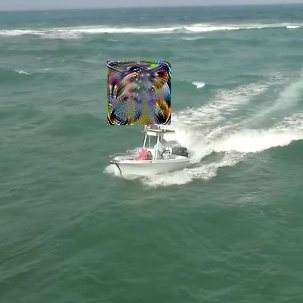
\includegraphics[width=0.11\textwidth]{images_imperceptible/imperceptible/AP.jpg}}
  \subfigure[Baseline-1]{\label{fig:imperceptibleb}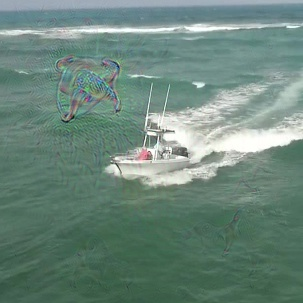
\includegraphics[width=0.15\textwidth]{images_imperceptible/imperceptible/UAP.jpg}}
  \subfigure[Baseline-2]{\label{fig:imperceptiblec}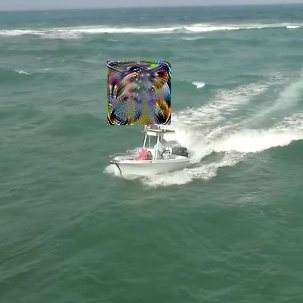
\includegraphics[width=0.15\textwidth]{images_imperceptible/imperceptible/AP.jpg}}
  \subfigure[Ours]{\label{fig:imperceptibled}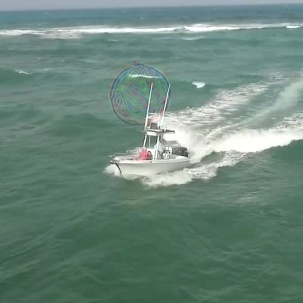
\includegraphics[width=0.15\textwidth]{images_imperceptible/imperceptible/Ours.jpg}}
  \caption{Visualization of perturbations on search images. Baseline-1 generates perturbations added to the whole search image and cannot perform targeted attacks. Baseline-2 pastes an obviously noticeable patch on the search image, which raises the risk of being suspected. Our method adds a small universal patch to the search image to perform targeted attacks.}
  \label{fig:imperceptible}
\end{figure}

\begin{table*}
  \centering
  \caption{Influence of the training iteration number on GOT-Val.}
  \begin{tabular}{rcccccccccccccccc} 
  \toprule
  \multicolumn{2}{r}{Iterations}     & 1     & 2     & 4     & 8     & 16    & 32    & 64    & 128   & 256   & 512   & 1024  & 2048  & 4096  & 8192  \\ 
  \midrule
  \multirow{2}{*}{Untargeted Attack} & AO    &  0.14 & 0.14 & 0.14 & 0.14 & 0.14 & 0.14 & 0.15 & 0.18 & 0.47 & 0.73 & 0.78 & 0.82 & 0.84 & 0.84  \\
                              & SR    &  0.1 & 0.1 & 0.1 & 0.1 & 0.1 & 0.1 & 0.11 & 0.15 & 0.49 & 0.78 & 0.84 & 0.88 & 0.89 & 0.89    \\ 
  \midrule
  \multirow{2}{*}{Targeted Attack} & AO   & 0.76 & 0.77 & 0.76 & 0.76 & 0.76 & 0.76 & 0.75 & 0.73 & 0.48 & 0.27 & 0.22 & 0.17 & 0.15 & 0.15    \\
                              & SR   & 0.89 & 0.9 & 0.89 & 0.89 & 0.9 & 0.89 & 0.88 & 0.86 & 0.53 & 0.25 & 0.18 & 0.14 & 0.12 & 0.12    \\ 
  \midrule
  \multicolumn{2}{r}{SSIM of $\delta$}&   1 & 1 & 1 & 1 & 0.99 & 0.99 & 0.97 & 0.94 & 0.88 & 0.84 & 0.82 & 0.81 & 0.8 & 0.79\\
  \midrule
  % \multicolumn{2}{c|}{SSIM of $p$}      &  0.98 & 0.98 & 0.98 & 0.98 & 0.98 & 0.98 & 0.98 & 0.98 & 0.98 & 0.97 & 0.98 & 0.98 & 0.98 & 0.98\\
  \multicolumn{2}{r}{SSIM of $p$}      &  0.98 & 0.98 & 0.98 & 0.98 & 0.98 & 0.98 & 0.93 & 0.78 & 0.56 & 0.50 & 0.51 & 0.52 & 0.53 & 0.56\\
  \bottomrule
  \end{tabular}
  \label{tab:iter}
\end{table*}

\begin{table}[h]
  \centering
  \caption{Overall attack results on VOT2016, VOT2018, VOT2019 and UAV123.}
  \begin{tabular}{rrcc}
  \toprule
  Benchmarks & Metrics & Before Attack    & Untargeted Attack  \\
  \midrule
  \multirow{2}{*}[-6pt]{VOT2016} 
  & Accuracy   & 0.626 & 0.393\\
  & Robustness & 0.144 & 9.061\\
  & EAO        & 0.460 & 0.007\\
  \midrule
  \multirow{2}{*}[-6pt]{VOT2018} 
  & Accuracy   & 0.587 & 0.342\\
  & Robustness & 0.183 & 8.981\\
  & EAO        & 0.426 & 0.007\\
  \midrule
  \multirow{2}{*}[-6pt]{VOT2019} 
  & Accuracy   & 0.556 & 0.345\\
  & Robustness & 0.537 & 8.824\\
  & EAO        & 0.243 & 0.010\\
  \midrule
  \multirow{3}{*}[+6pt]{UAV123} 
  & AO  & 0.623 & 0.064\\
  & Precision & 0.781 & 0.187\\
  \bottomrule
  \end{tabular}
  \label{tab:benchmark results1}
\end{table}

\begin{table}[t]
  \centering
  \caption{Overall attack results on OTB-15, GOT-Val and LaSOT.}
  \begin{tabular}{rrccc}
  \toprule
  \multirow{2}{*}{Benchmarks} & \multirow{2}{*}{Metrics} & Before    & Targeted & Untargeted  \\
                            &                         & Attack & Attack & Attack     \\ 
  \midrule
  \multirow{2}{*}{OTB-15} 
  & AO   & 0.642 & 0.063 & 0.759\\
  & Precision & 0.861 & 0.092 & 0.795\\
  \midrule
  \multirow{2}{*}{GOT-Val} 
  & SR & 0.897 & 0.123 & 0.890\\
  & AO & 0.760 & 0.153 & 0.840 \\
  \midrule
  \multirow{3}{*}{LaSOT} 
  & Precision  & 0.514 & 0.046 & 0.605\\
  & Norm. Prec.& 0.551 & 0.048 & 0.702\\
  & AO         & 0.525 & 0.069 & 0.691\\
  %& Succ. rate  & 0.626 & 0.016 & 0.834\\
  \midrule
  \multicolumn{2}{r}{FPS} & 58 & 58 & 58\\
  \bottomrule
  \end{tabular}
  \label{tab:benchmark results}
\end{table}

\subsection{Compared With Baselines}

We compare our attack method with two baseline methods (See Table \ref{tab:imperceptible}).
\textbf{Baseline-1} performs untargeted attacks based on the UAP \cite{UAP} method. The difference between Baseline-1 and our method is that, Baseline-1 generates perturbations added to the whole search image and cannot perform targeted attacks, while our method adds a small universal patch to the search image to perform targeted attacks (see Figure \ref{fig:imperceptible}).
\textbf{Baseline-2} performs targeted attacks based on the adversarial patch \cite{patch} method. The differences between Baseline-2 and our method include: (1) Baseline-2 pastes an adversarial patch on the search image without the $l_p\text{-norm}$ constrain while our method adds the patch onto the search image with the $l_p\text{-norm}$ constrain. 
%\uline{
(2) Baseline-2 uses the clean template image while we add translucent perturbations onto the template image. As a consequence, Baseline-2 generates an obviously noticeable patch while ours are translucent as shown in Figure \ref{fig:imperceptible}.
%}
%Moreover, both the untargeted attack performance and the targeted performance of our method are better than Baseline-2 as shown in Table \ref{tab:imperceptible}.

\subsection{Attack Results on the Evaluation Benchmarks}

\textit{Overall Attack Results} We test the performance of our targeted attack method on the evaluation benchmarks and gather the overall results in Table \ref{tab:benchmark results1} and Table \ref{tab:benchmark results}. It is shown that the base tracker SiamFC++ can achieve state-of-the-art performance on all the evaluation benchmarks and run in real time (at about 58 fps on a GTX 1080Ti GPU). However this real-time performance requires the computationally intensive tracking system to occupy most of the computational resources, and thus it is appealing to develop a virtually costless attack method to fool the tracking system without scrambling for the resources. As shown in Table \ref{tab:benchmark results}, our attack method can satisfy this appealing demand and fool the SiamFC++ tracker effectively by misleading the tracker to follow a predefined \textit{fake trajectory}. Moreover, the high AO and Precision performance with respect to the \textit{fake trajectory} indicates a more effective attack without raising any suspicion (see Figure \ref{fig:vis1}).

% \begin{figure}[t]
%   \centering
%   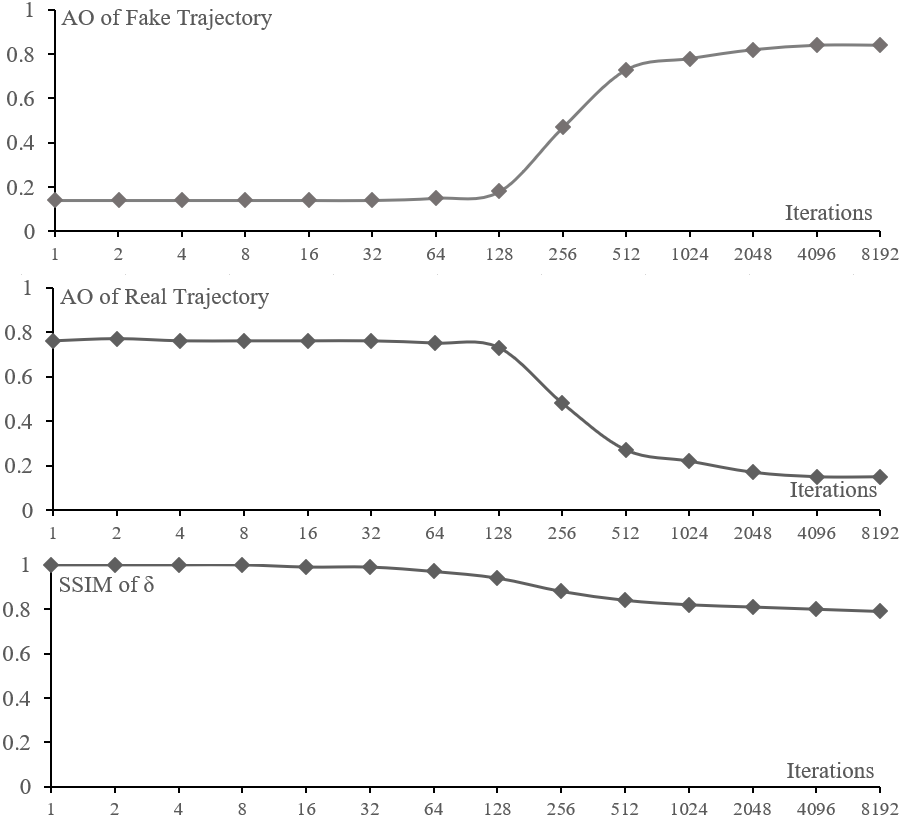
\includegraphics[width=0.48\textwidth]{images_imperceptible/iter.png}
%   \caption{Influence of the training iteration number on GOT-Val.} 
%   \label{fig:iter}
% \end{figure}

\textit{Ablation Study: Influence of Training Iterations} Table \ref{tab:iter} demonstrates the influence of the number of training iterations on the attack performance. It can be observed that as the number of iterations increases, the AO score with respect to the fake trajectory increases significantly, while the AO score with respect to the real trajectory decreases significantly. This demonstrates the effectiveness of the end-to-end training process proposed in this paper. After about 8,000 training iterations, the resulting perturbation prevents the tracker from tracking most of the targets in GOT-Val, and the AO with respect to the real trajectory decreases from 0.760 to 0.153. Note that the AO decreases significantly faster at the beginning (training iterations less than 2048). This demonstrates the fast convergence capability of our end-to-end training scheme.

To verify whether the perturbations generated for the template images are difficult to perceive, we evaluate the quality of the input images after the perturbations by the metric SSIM. As shown in Table \ref{tab:iter}, the SSIM value of the perturbed images gradually decreases as the training proceeds, which indicates that the difference between the perturbed images and the original images gradually increases due to the learned adversarial perturbation being added to the clean images. The SSIM value ranges from 0 to 1. If the SSIM is close to 1, the difference between the perturbed images and the original images is small. The SSIM value of the perturbed template image is 0.79, and the SSIM of the perturbed search image (calculated on the subregion where the patch is placed) is 0.56. 

\begin{figure}[t]
  \centering
  \subfigure[FAN]{\label{fig:a1}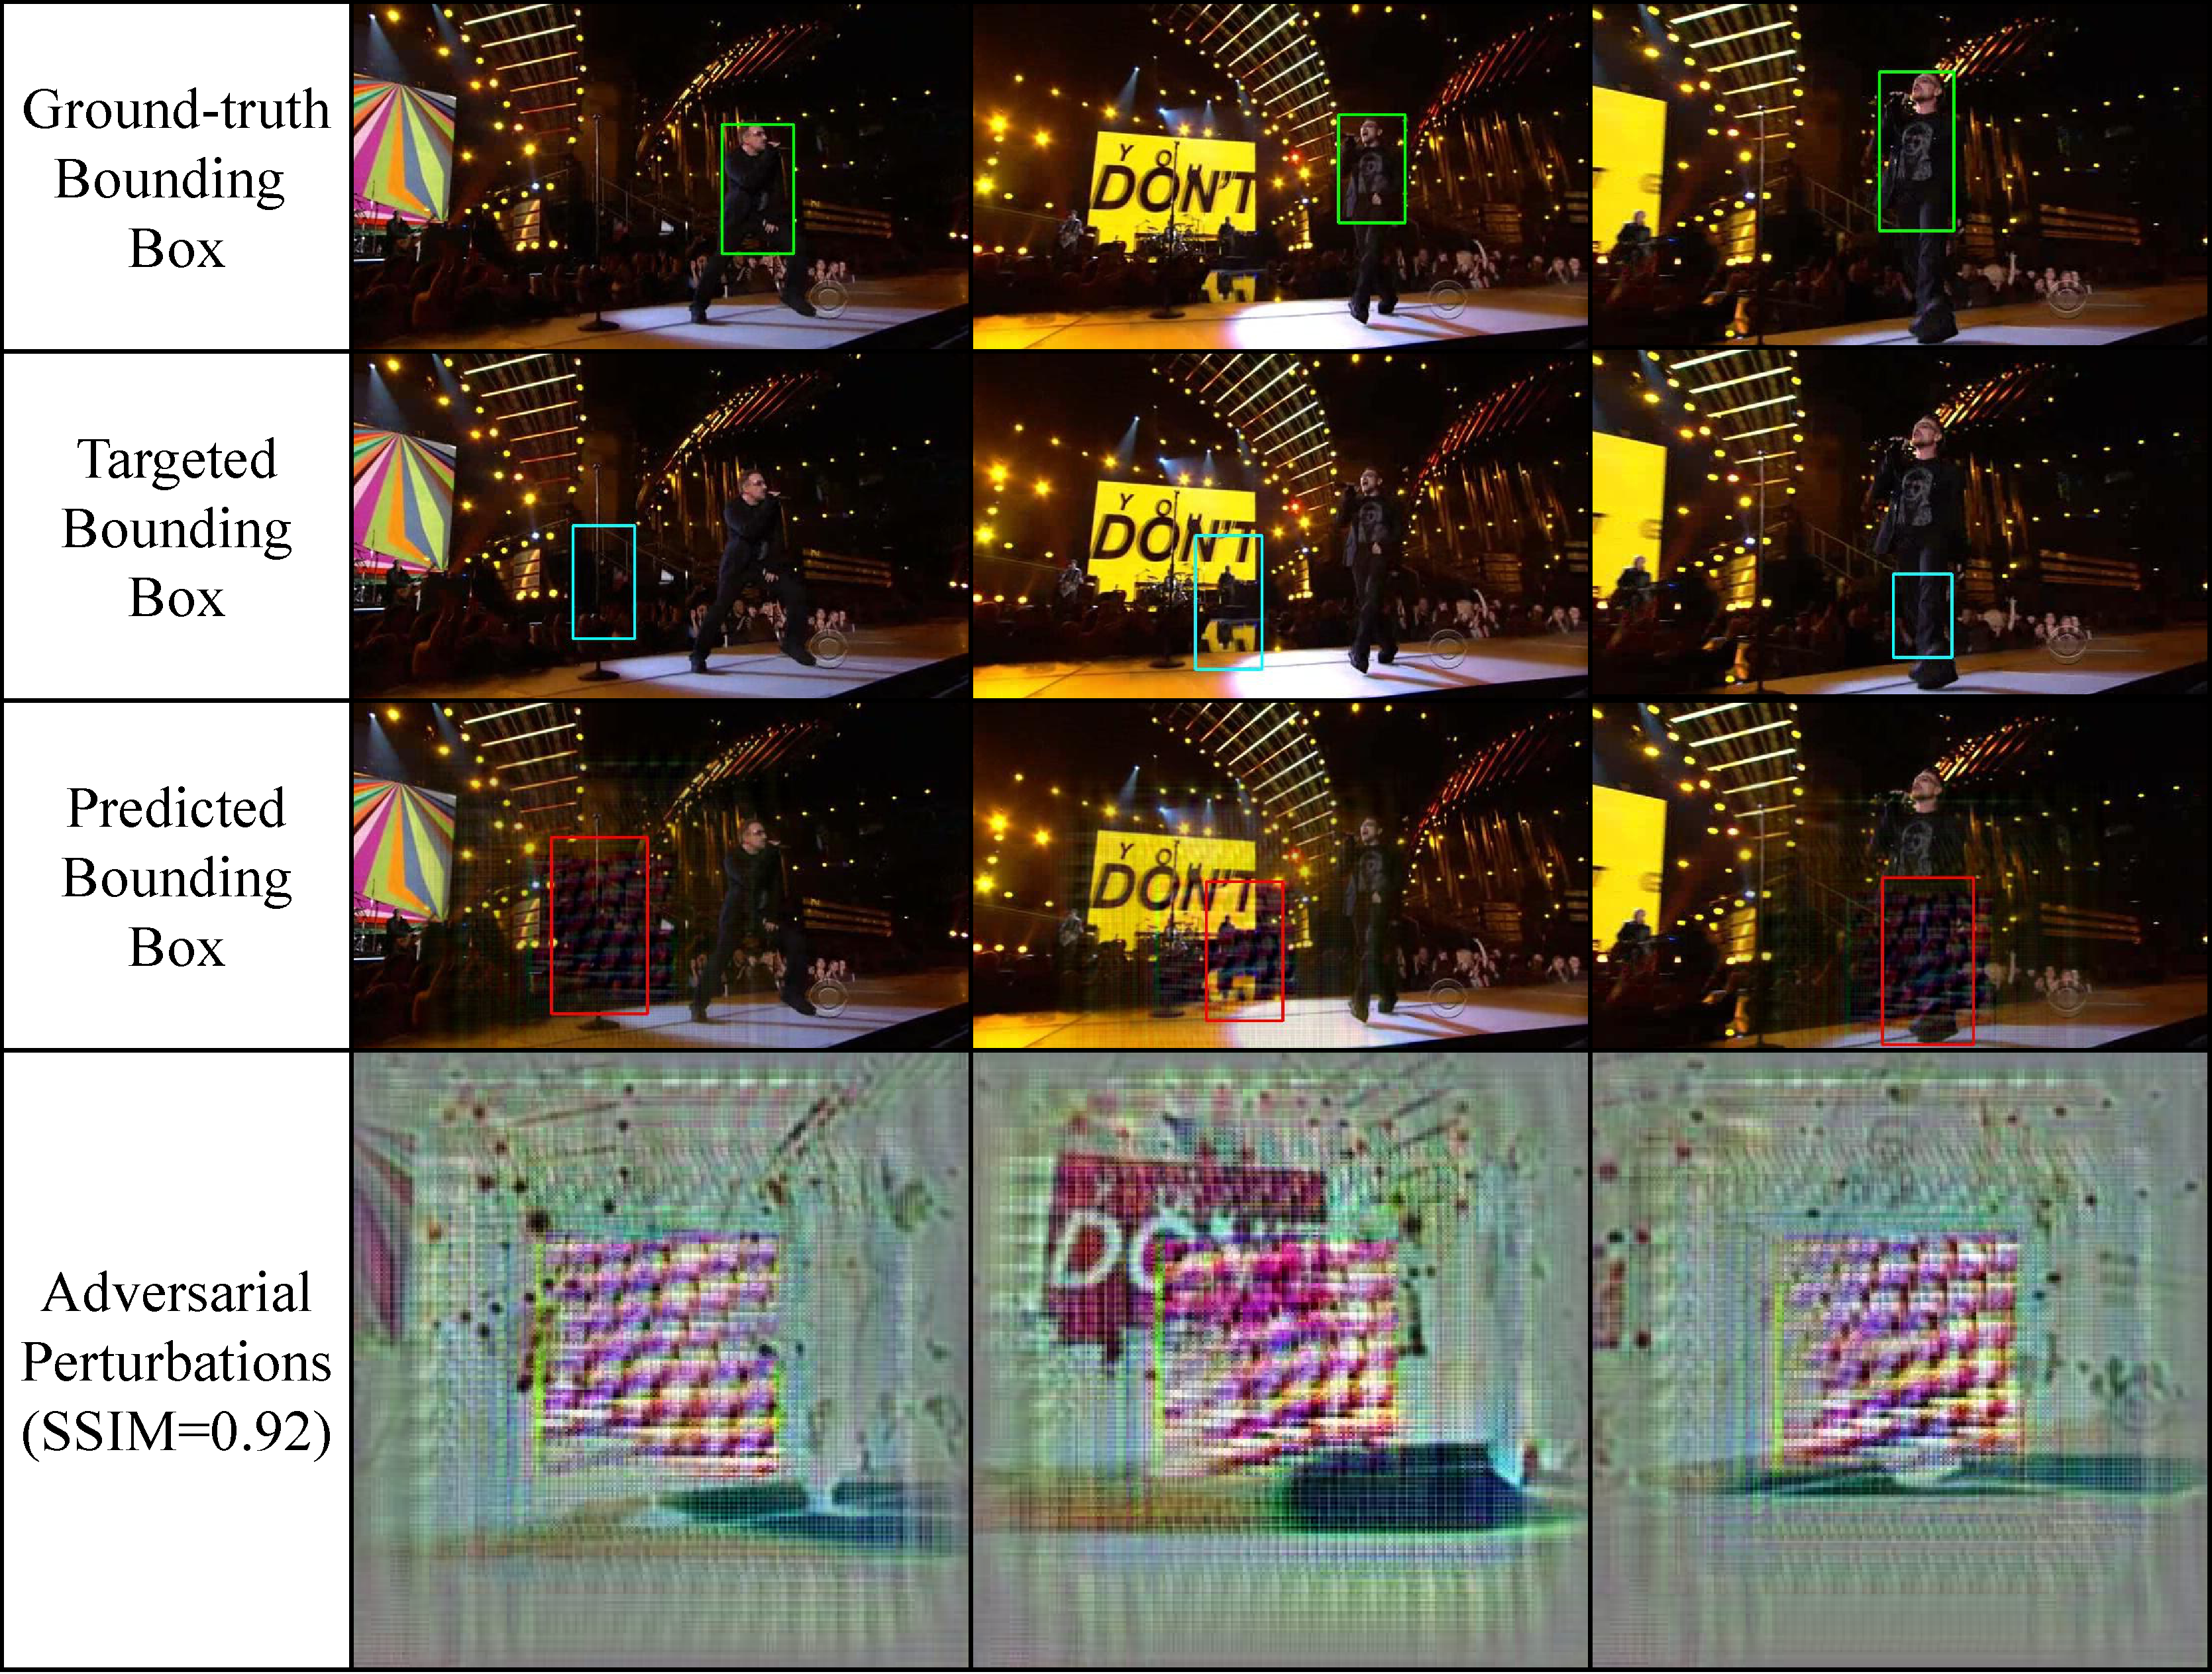
\includegraphics[width=0.48\textwidth]{images_imperceptible/FAN.pdf}}
  \subfigure[Ours]{\label{fig:b1}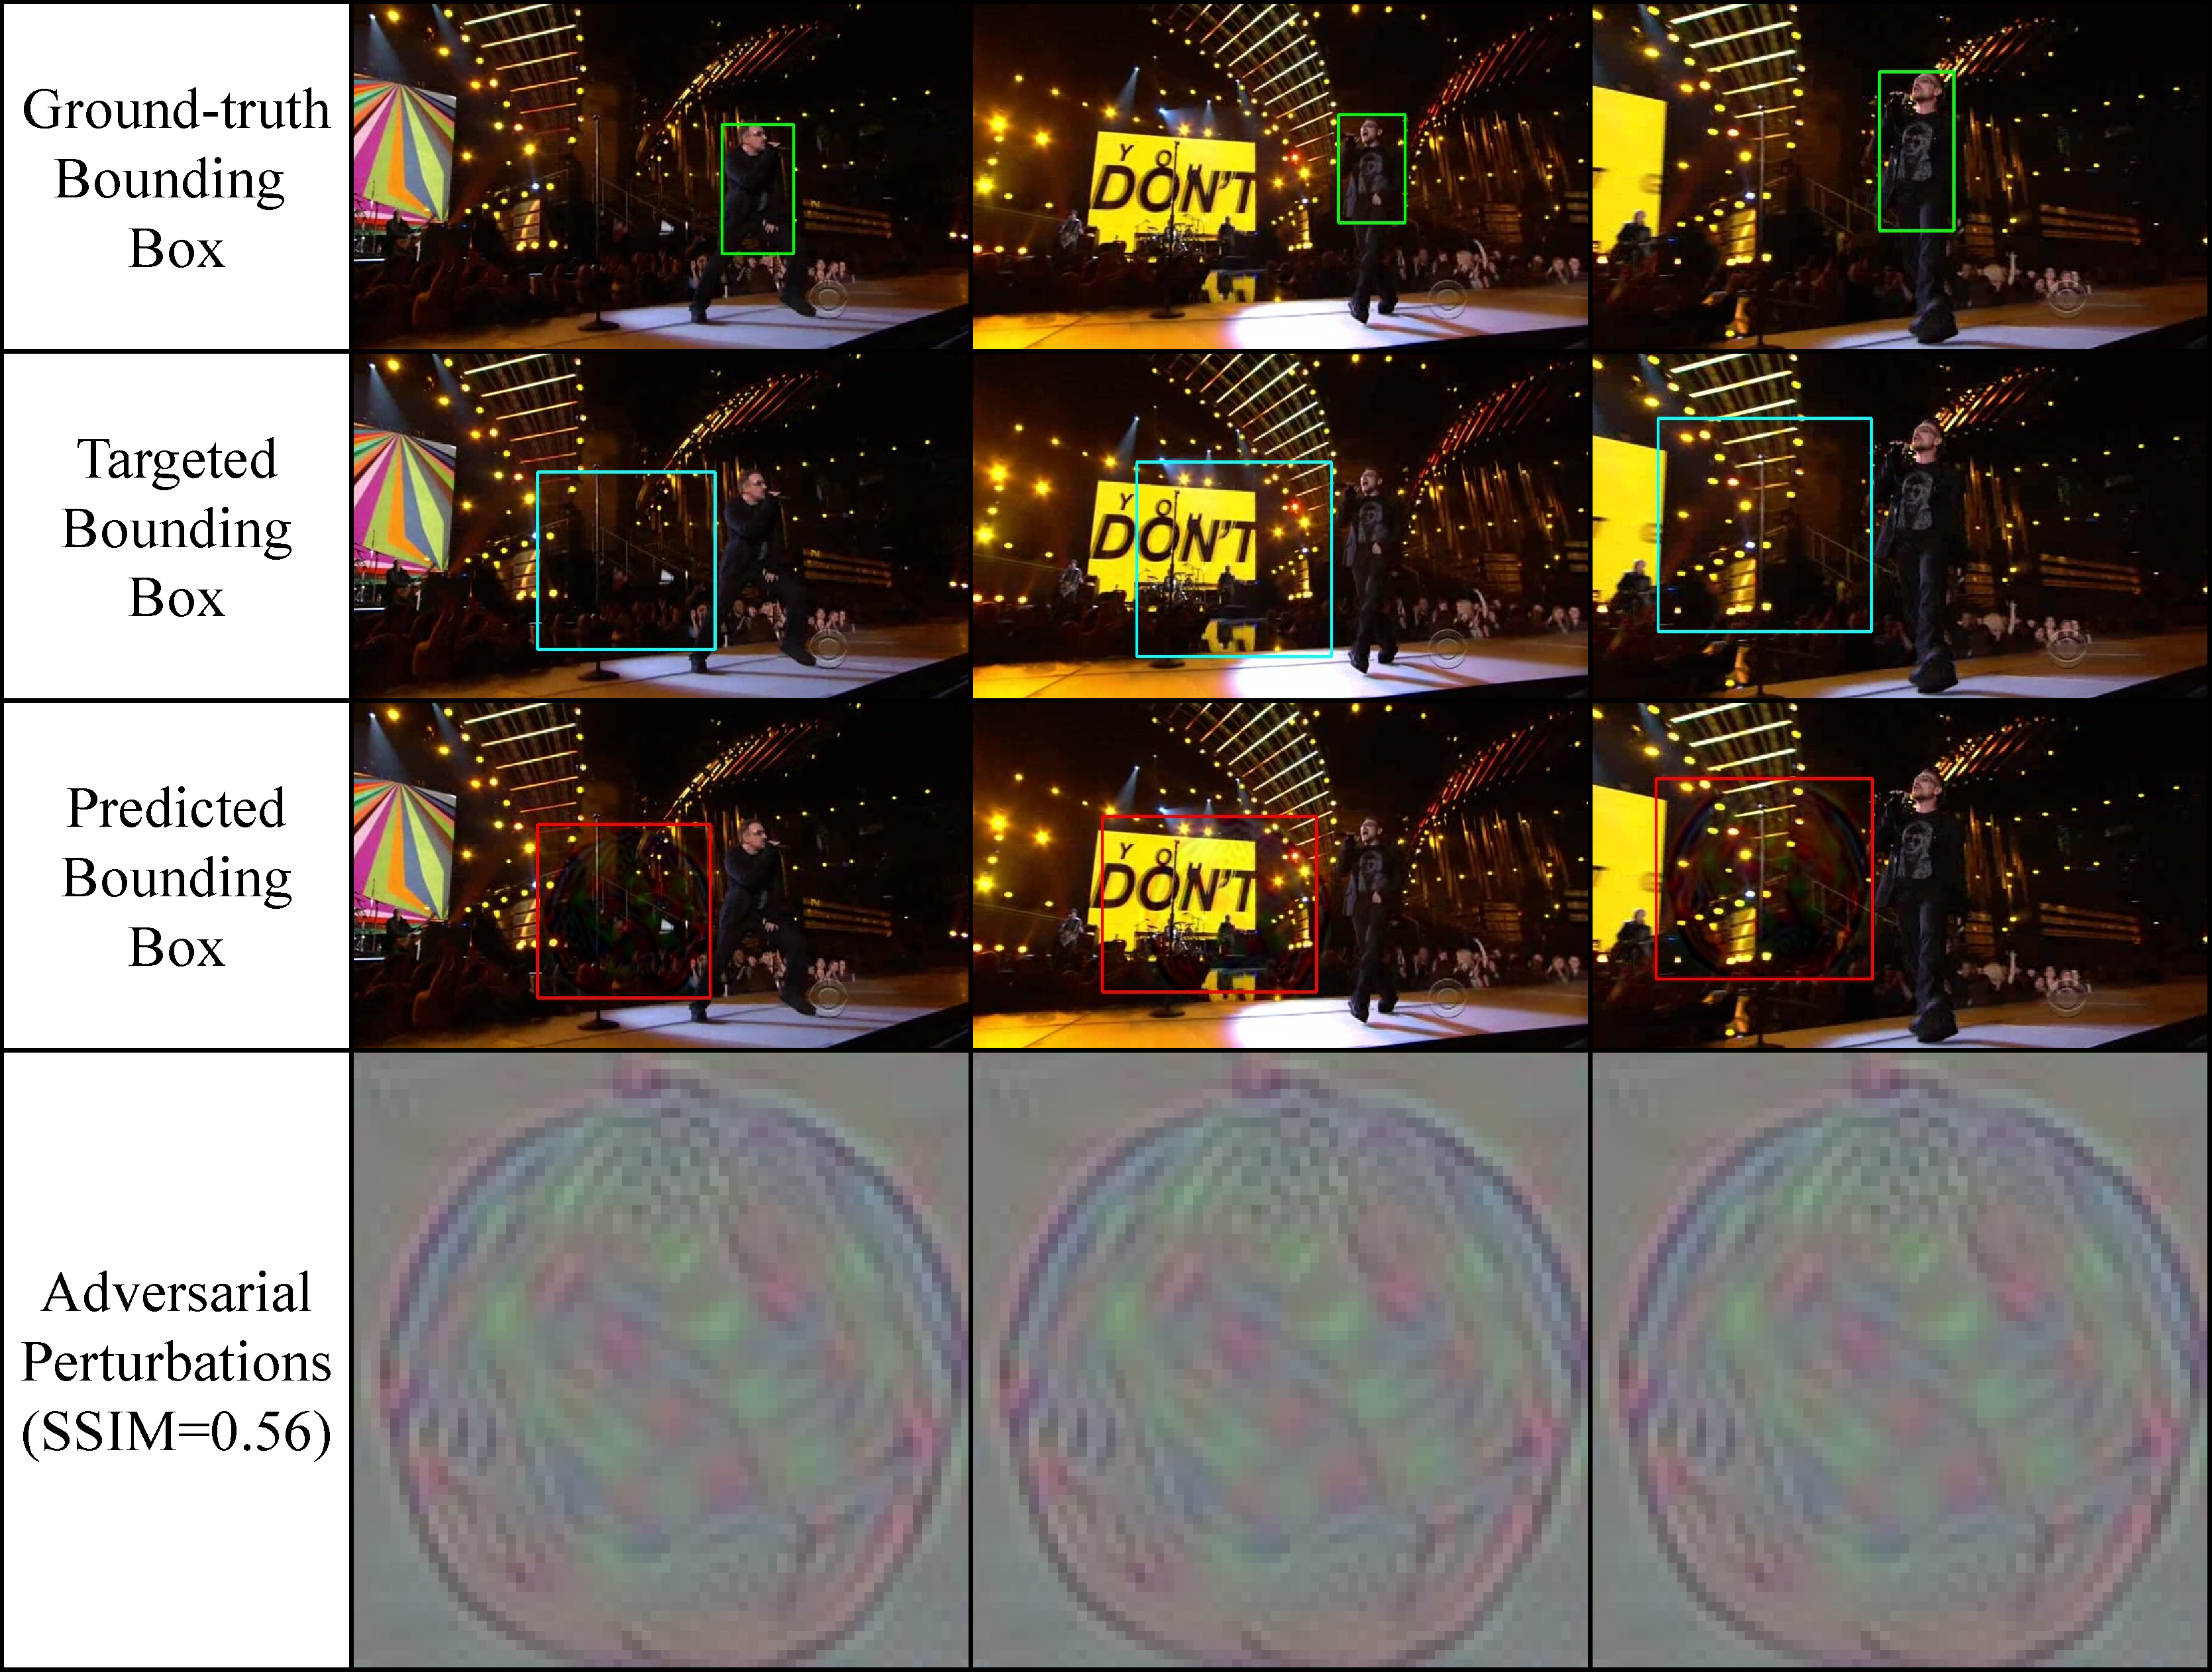
\includegraphics[width=0.48\textwidth]{images_imperceptible/Ours.pdf}}
  \caption{The results under targeted attacks compared with FAN \cite{FAN}.  FAN crafts the perturbations for each video independently, which comes at a non-negligible computational cost. To achieve video-agnostic universal attack on Siamese trackers, we relax the constraint on the value of the perturbation, achieving a balance between the attack efficiency and the perturbation perceptibility.}
  \label{fig:vis_fan}
\end{figure}

%\uline{
% 为了进一步分析扰动的可感知性,我们在图中与FAN进行了对比。
To further analyze the perceptibility of perturbations, we compare our method with FAN in Figure \ref{fig:vis_fan}.
% We visualize the perturbed frames ($3^{rd}$ row of Figure \ref{fig:vis}) of OTB2015 dataset, Singer2 video. 
As shown in Figure \ref{fig:vis_fan}, both FAN \cite{FAN} and our method can perform targeted attack. 
% 添加了由FAN生成的扰动的OTB的SSIM下降至0.92。添加了我们的扰动的OTB的SSIM下降至0.56。
The SSIM of OTB2015 perturbed by FAN drops to 0.92, while the SSIM perturbed by our method drops to 0.56.
% 这是因为FAN为每帧产生独立的扰动,而我们的扰动是通用的,因此我们的任务比FAN更难,导致我们的扰动值更大。
This is because FAN generates independent perturbations for each frame, while our perturbations are universal, which is a more difficult task, resulting in larger values for our perturbations.
By relaxing the constraint on the value of the perturbation, we can achieve better targeted attack performance on OTB2015.
Our method achieves a precision score of 0.795, compared to 0.420 for FAN.
What's more, our method can perform universal attack, both with respect to the data and the network architectures.
%}

\begin{table}[t]
  \centering
  \caption{Analysis of the impact of each loss component on GOT-Val.}
  \begin{tabular}{ccccccc} 
  \toprule
  \multirow{2}{*}[-2pt]{$L_{\text{cls}}$}     & \multirow{2}{*}[-2pt]{$L_{\text{quality}}$} & \multirow{2}{*}[-2pt]{$L_{\text{reg}}$} & \multicolumn{2}{c}{Trageted Attack}          & \multicolumn{2}{c}{Untargeted Attack}           \\ 
  \cmidrule{4-7}
                         &                    &                    & AO                    & SR                    & AO                    & SR                     \\ 
  \midrule
  \checkmark   &    &    & 0.643  & 0.726    & 0.282 & 0.274   \\
     & \checkmark   &    & 0.148  & 0.110    & 0.747 & 0.882   \\
     &    & \checkmark   & 0.726  & 0.762    & 0.243 & 0.238   \\
  \checkmark   & \checkmark   & \checkmark   & 0.840  & 0.890    & 0.153 & 0.123   \\ \bottomrule
  \end{tabular}
  \label{tab:loss}
\end{table}

\begin{figure}[t!]
  \begin{center}
    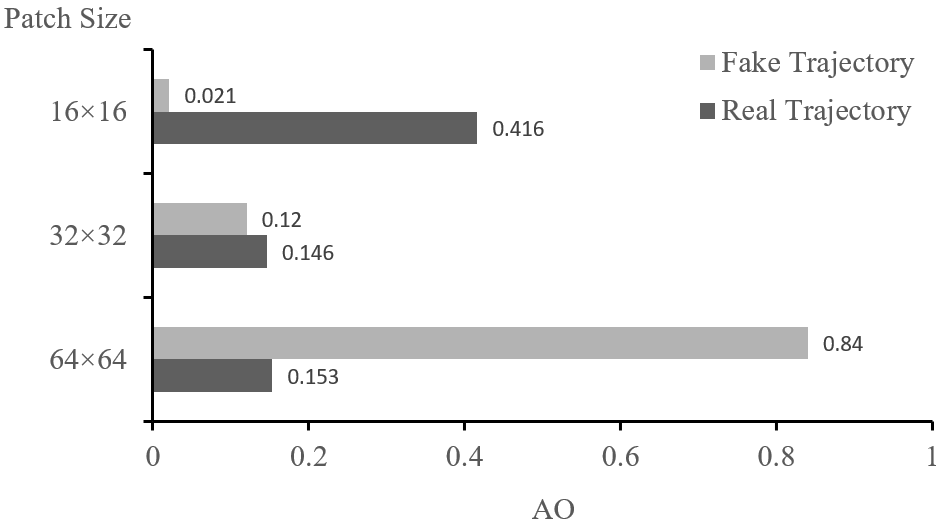
\includegraphics[width=0.48\textwidth]{images_imperceptible/patch_size/patch_size.png}
  \end{center}
  \caption{AO with respect to the real/fake trajectory on perturbed GOT-Val dataset. The 32-by-32 patch can make the AO score drop dramatically to 0.146 and its area only accounts for 1\% of the search image area.}
  \label{fig:patch_size_table}
\end{figure}

% \begin{figure}[t]
%   \centering
%   \subfigure[64$\times$64]{\label{fig:a}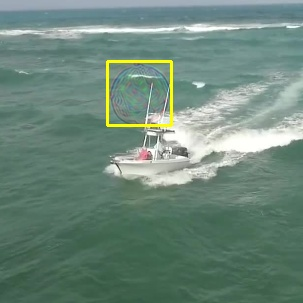
\includegraphics[width=0.15\textwidth]{images_imperceptible/patch_size/64.jpg}}
%   \subfigure[32$\times$32]{\label{fig:b}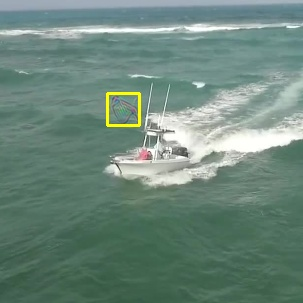
\includegraphics[width=0.15\textwidth]{images_imperceptible/patch_size/32.jpg}}
%   \subfigure[16$\times$16]{\label{fig:c}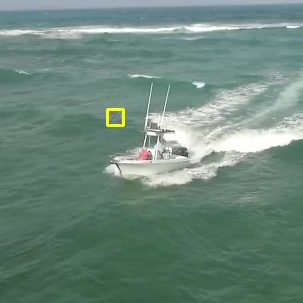
\includegraphics[width=0.15\textwidth]{images_imperceptible/patch_size/16.jpg}}
%   \caption{Adversarial patches of different sizes.}
%   \label{fig:patch_size_vis}
% \end{figure}

\begin{table}[t]
  \centering
  \caption{Transferability to different backbones on GOT-Val. The original perturbations are trained on SiamFC++\_GoogleNet, then we directly apply the perturbations to two more different backbones of SiamFC++, \ie, ShuffleNet \cite{ShuffleNet} and AlexNet \cite{AlexNet}.}
  \begin{tabular}{rcccccc} 
  \toprule
  \multirow{2}{*}[-2pt]{Backbone} & \multicolumn{2}{c}{Before Attack} & \multicolumn{2}{c}{Untargeted Attack} & \multicolumn{2}{c}{Targeted Attack}  \\ 
  % \cmidrule(lr){2-3} \cmidrule(lr){4-5} \cmidrule(lr){6-7}
  \cmidrule{2-7}
                            & AO    & SR                           & AO    & SR                           & AO    & SR                           \\ 
  \midrule
  GoogLeNet                 & 0.760 & 0.897                        & 0.153 & 0.123                        & 0.840 & 0.890                        \\
  AlexNet                   & 0.720 & 0.850                        & 0.496 & 0.577                        & 0.327 & 0.336                        \\
  ShuffleNet                & 0.766 & 0.888                        & 0.496 & 0.557                        & 0.409 & 0.426                       \\
  \bottomrule
  \end{tabular}
  \label{tab:backbone}
\end{table}
\begin{table}[t!]
  \centering
  \caption{Transferability to different tracking architectures on OTB2015. The original perturbations are trained on SiamFC++\_GoogleNet, then we directly apply the perturbations to two more state-of-the-art anchor-based trackers: AlexNet-based SiamRPN \cite{SiamRPN} and ResNet-based SiamRPN++ \cite{SiamRPN++}.}
  \begin{tabular}{rcccc} 
  \toprule
  \multirow{2}{*}[-2pt]{Trackers} & \multicolumn{2}{c}{Before Attack} & \multicolumn{2}{c}{Untargeted Attack}  \\
  \cmidrule{2-5}
                            & AO & Precision              & AO & Precision                   \\
  \midrule
  SiamRPN++                 & 0.676   & 0.879                  & 0.418   & 0.556                       \\
  SiamRPN                   & 0.666   & 0.876                  & 0.483   & 0.643                       \\
  \bottomrule
  \end{tabular}
  \label{tab:arch}
\end{table}

\textit{Ablation Study: Influence of Training Loss} We implemented a series of experiments to analyze the contribution of each loss component. In Table \ref{tab:loss}, we report the attack results on the GOT-Val dataset. The AO score of the tracker with respect to the real trajectory decreases from 0.760 to 0.747 when adversarial information is generated using only quality assessment loss, indicating that quality assessment loss can cause a slight degradation in the performance of the tracker. This is because the perturbation information generated using quality assessment loss interferes with the tracker's ability to select the best target. However, the tracker's AO score with respect to the fake trajectory is only 0.148, indicating that the perturbations generated using quality assessment loss alone can barely cause the tracker to follow the specified trajectory. When the adversarial information is generated using only regression loss, the AO score of the tracker with respect to the real trajectory decreases from 0.760 to 0.243, indicating that regression loss can cause a large degradation in the tracker's performance. This is because the perturbation information generated using regression loss corrupts the tracker's ability to predict the accurate bounding box position. When adversarial information is generated using only classification loss, the tracker's AO score decreases from 0.760 to 0.282 with respect to the real trajectory and the AO with respect to the fake trajectory is up to 0.643. This is because the perturbation information generated using classification loss causes the tracker to localize to the fake target instead of the real target's location. In conclusion, all loss terms are beneficial, and the classification/regression term is more important than the quality assessment term.

% \begin{figure*}[t!]
%   \begin{center}
%     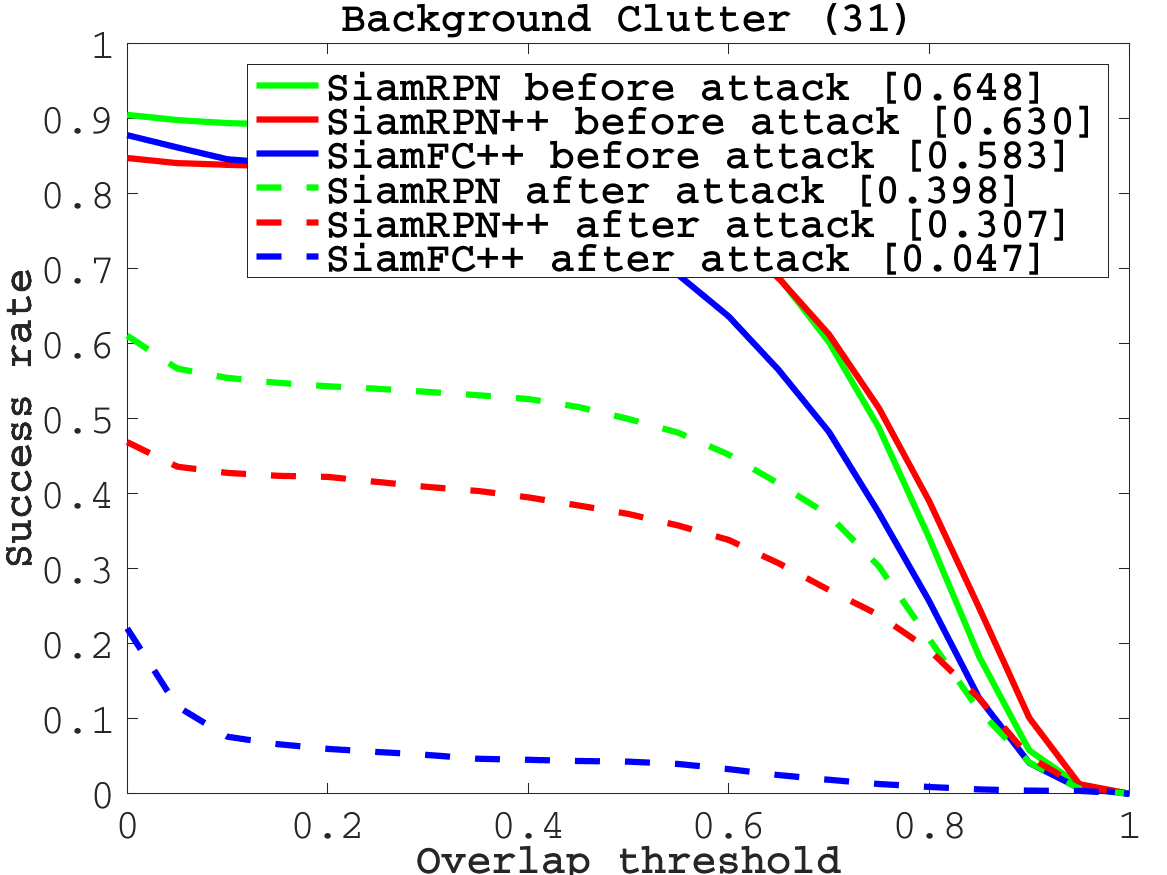
\includegraphics[width=0.32\textwidth]{images_imperceptible/OTB2015/success_plot_OPE_OTB100_BC.png}
%     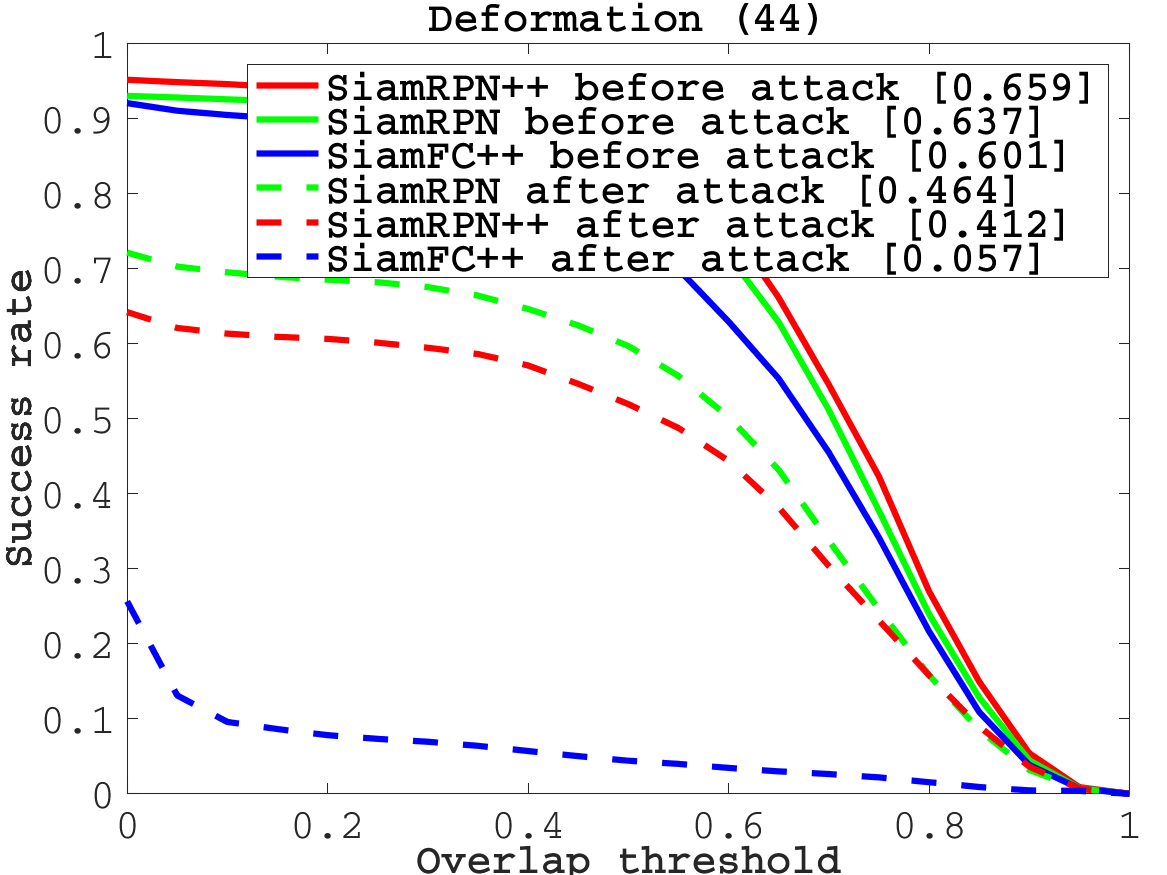
\includegraphics[width=0.32\textwidth]{images_imperceptible/OTB2015/success_plot_OPE_OTB100_DEF.png}
%     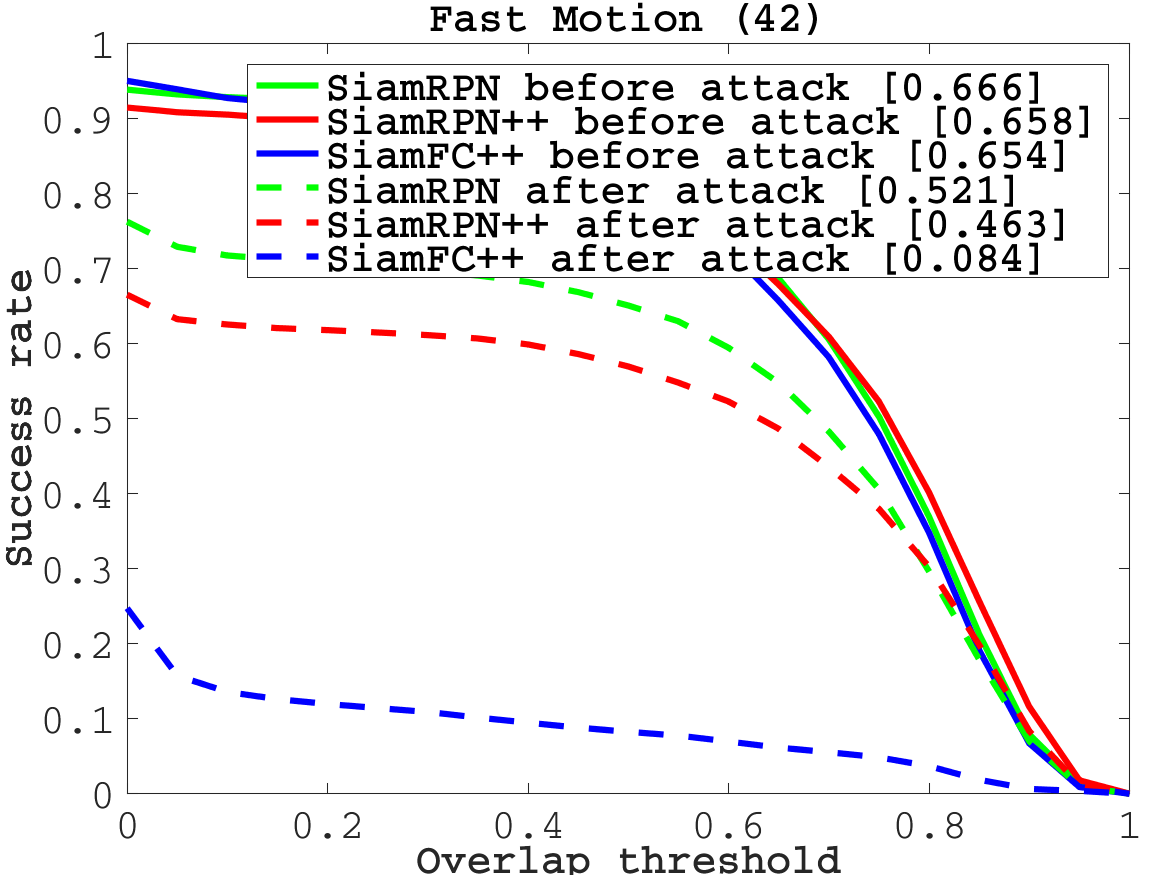
\includegraphics[width=0.32\textwidth]{images_imperceptible/OTB2015/success_plot_OPE_OTB100_FM.png}
%     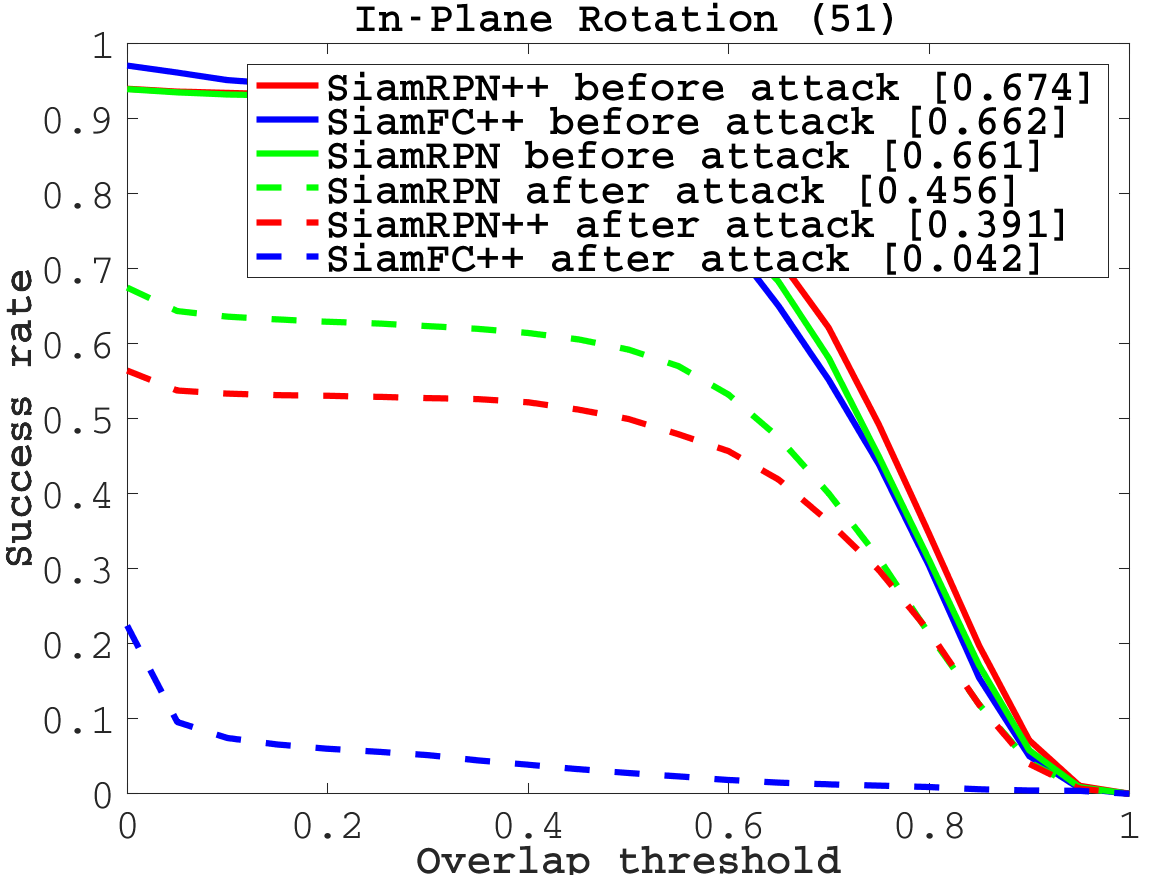
\includegraphics[width=0.32\textwidth]{images_imperceptible/OTB2015/success_plot_OPE_OTB100_IPR.png}
%     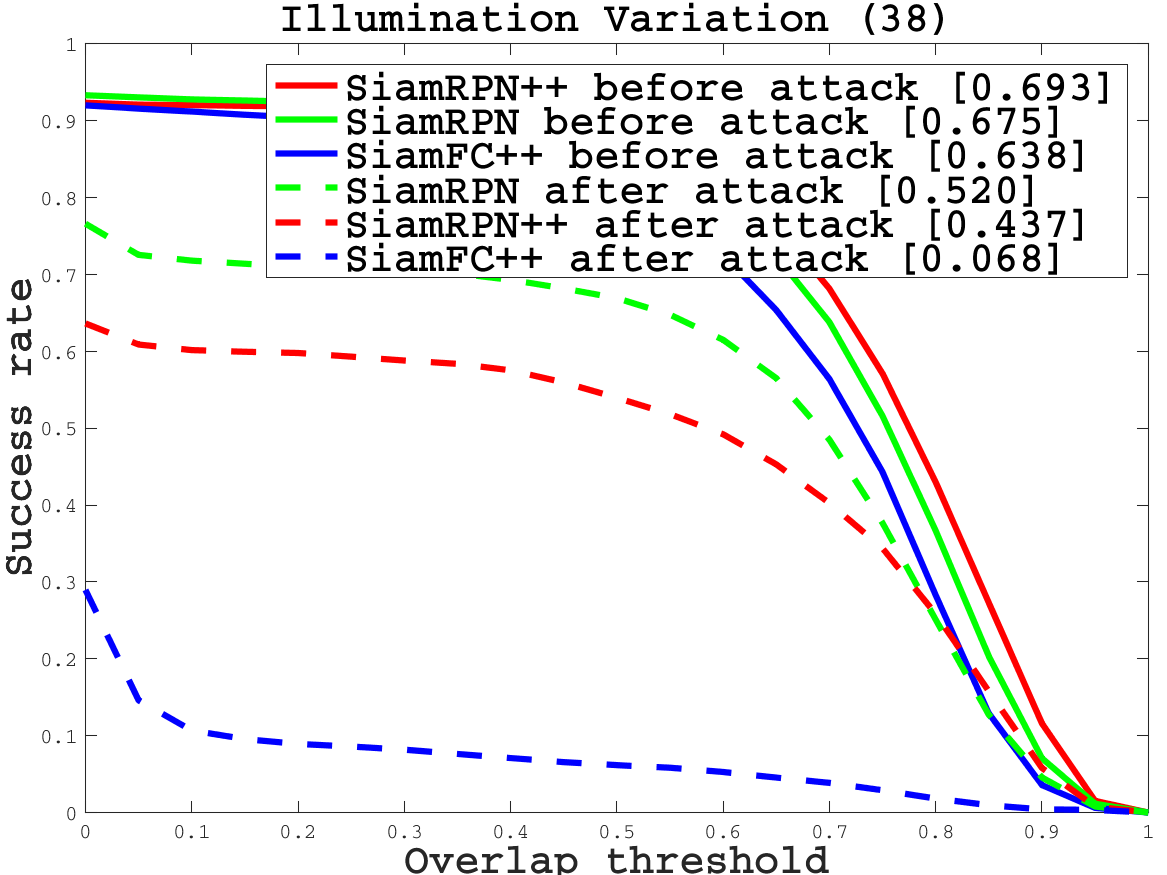
\includegraphics[width=0.32\textwidth]{images_imperceptible/OTB2015/success_plot_OPE_OTB100_IV.png}
%     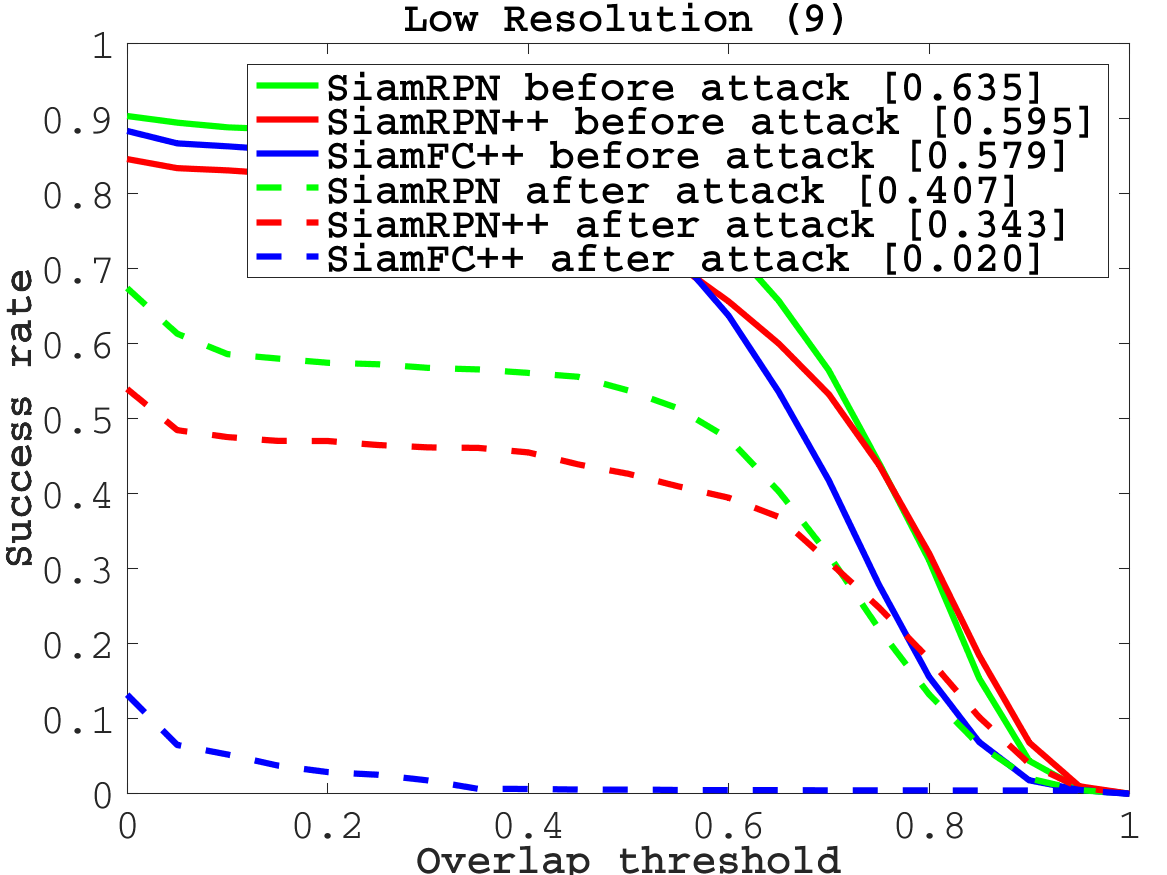
\includegraphics[width=0.32\textwidth]{images_imperceptible/OTB2015/success_plot_OPE_OTB100_LR.png}
%     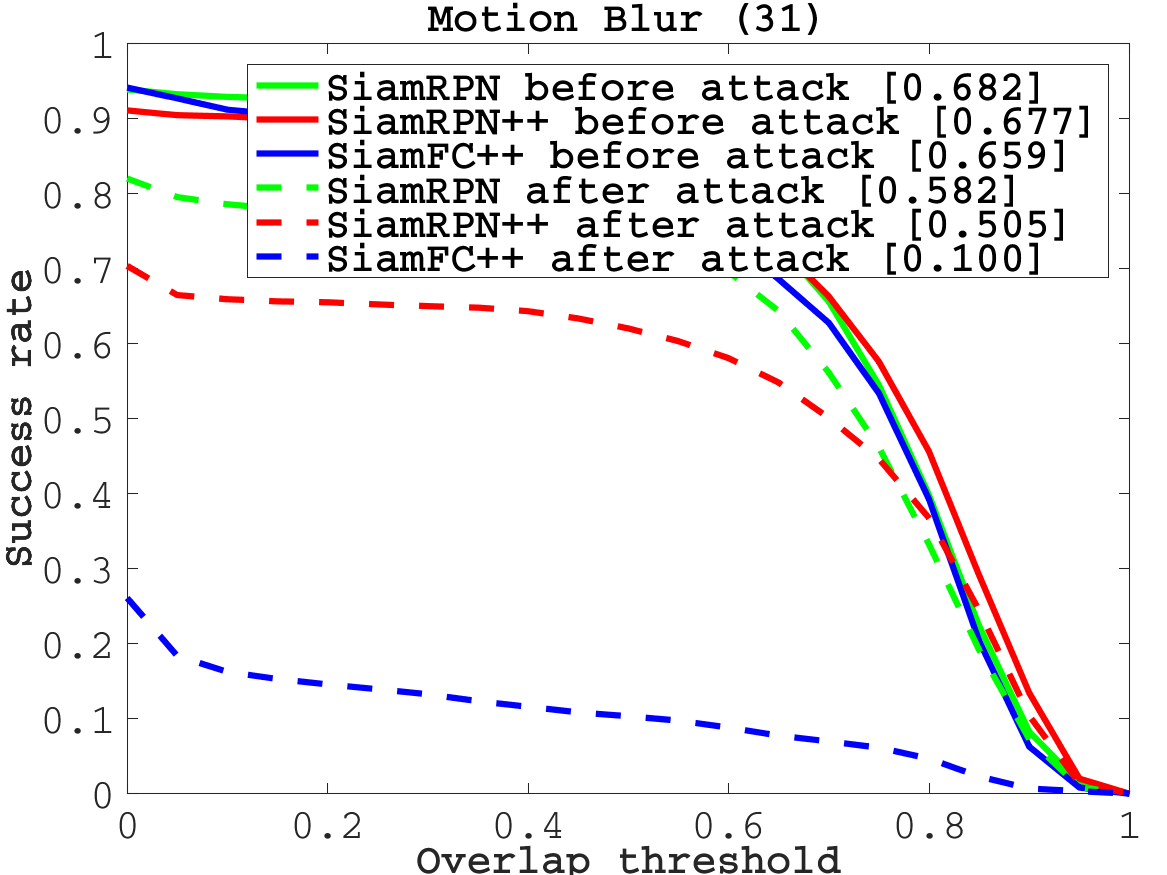
\includegraphics[width=0.32\textwidth]{images_imperceptible/OTB2015/success_plot_OPE_OTB100_MB.png}
%     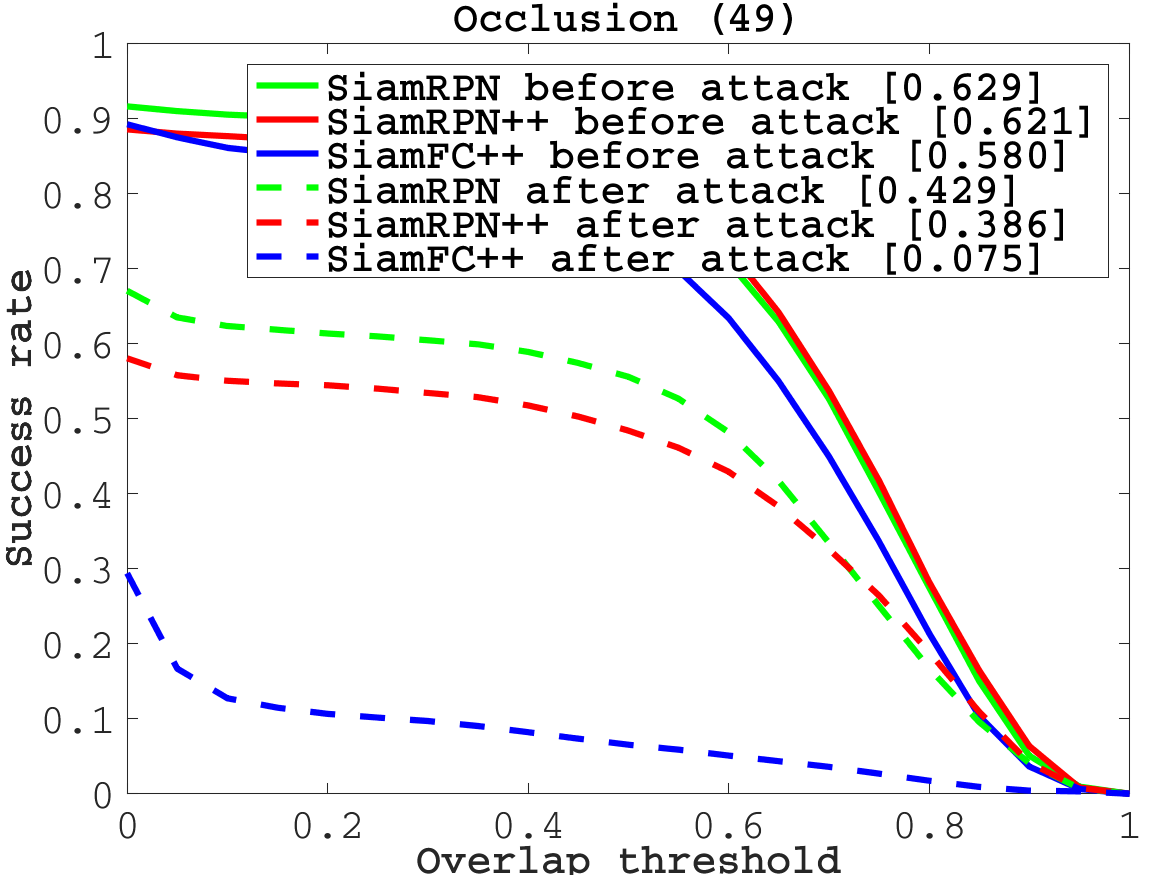
\includegraphics[width=0.32\textwidth]{images_imperceptible/OTB2015/success_plot_OPE_OTB100_OCC.png}
%     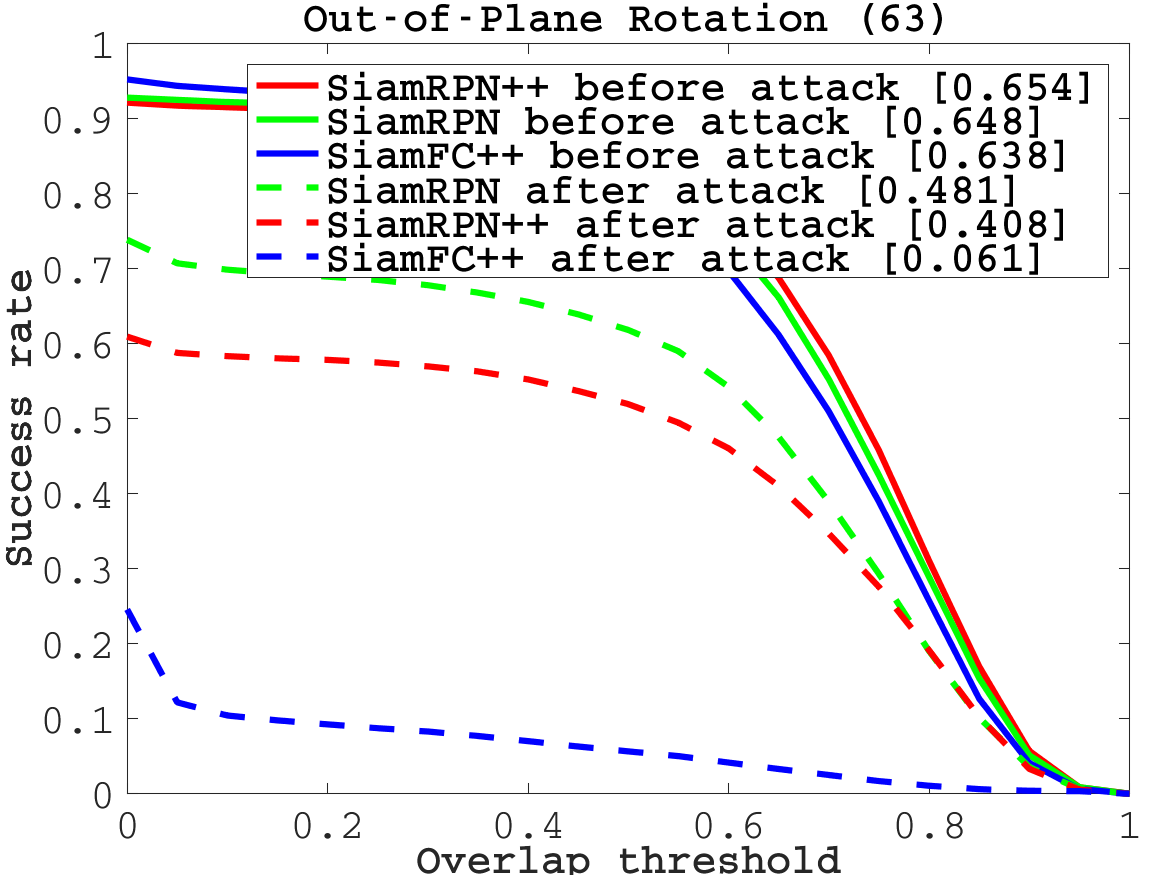
\includegraphics[width=0.32\textwidth]{images_imperceptible/OTB2015/success_plot_OPE_OTB100_OPR.png}
%     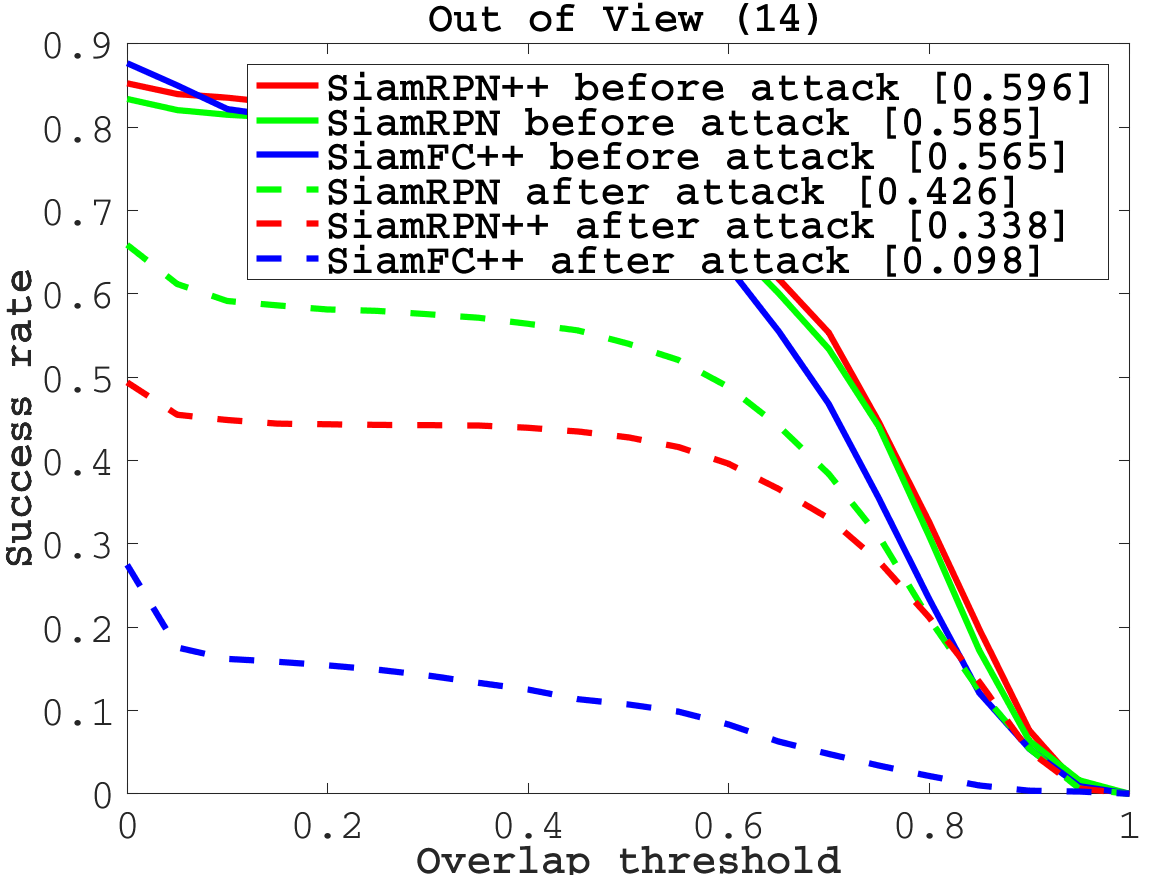
\includegraphics[width=0.32\textwidth]{images_imperceptible/OTB2015/success_plot_OPE_OTB100_OV.png}
%     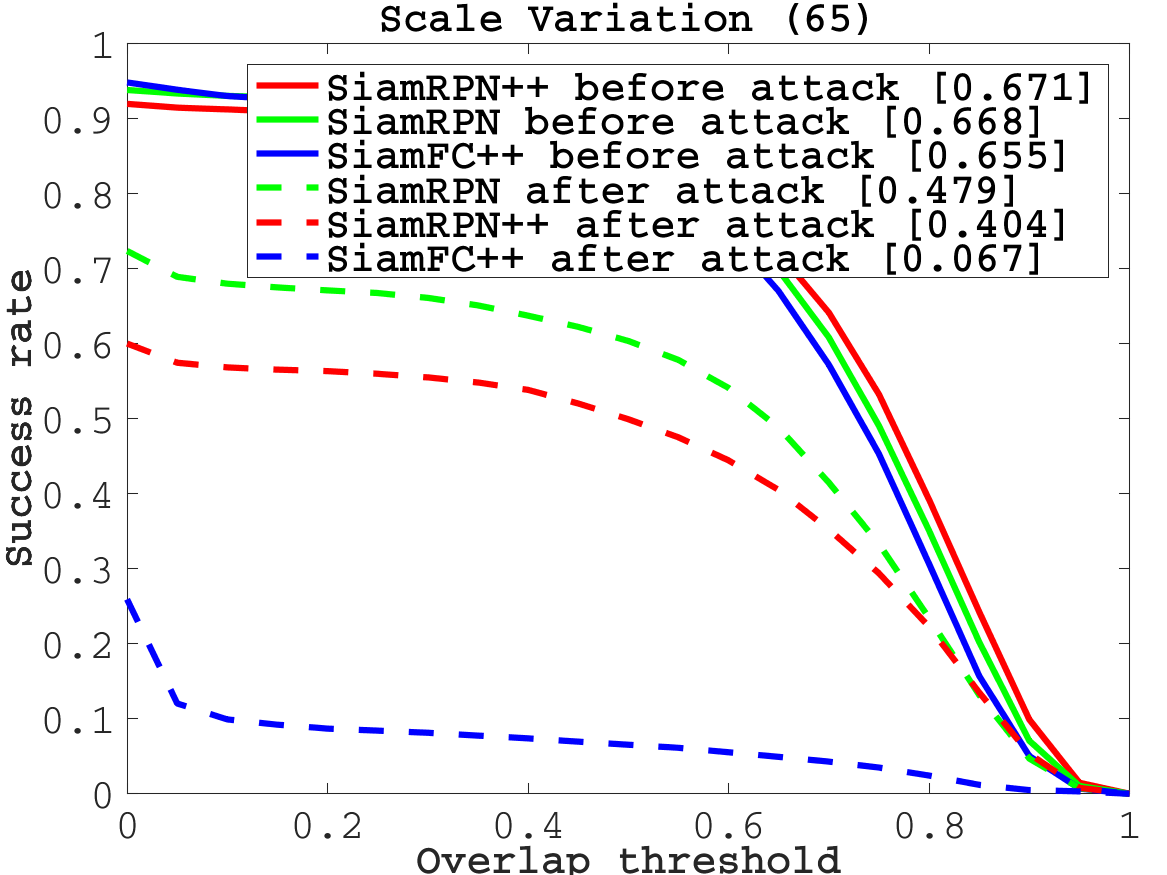
\includegraphics[width=0.32\textwidth]{images_imperceptible/OTB2015/success_plot_OPE_OTB100_SV.png}
%   \end{center}
%       \caption{Untargeted attack results of the different trackers under the 11 attributes: out-of-view (OV), occlusion (OCC), illumination variation (IV), out-of-plane rotation (OPR), scale variation (SV),deformation (DEF), low resolution (LR), fast motion (FM), background clutters (BC), motion blur (MB), and in-plane rotation (IPR). The results show good transferability of our attacks to different tracking architectures, even if the generated perturbations are applied to anchor-based trackers.}
%   \label{fig:attr}
% \end{figure*}

\textit{Ablation Study: Influence of the Adversarial Patch Size} 
It's important to make the size of the adversarial patch small to avoid suspicion. In our experiment, we produce three different sizes of the adversarial patch, namely, 64-by-64, 32-by-32 and 16-by-16 to test the efficiency of their attacks. We evaluate the AO score of SiamFC++ on the perturbed GOT-Val dataset.
As shown in Figure \ref{fig:patch_size_table}, the 32-by-32 patch can make the AO score drop dramatically to 0.146 and its area only accounts for 1\% of the search image area.

\textit{Ablation Study: Performance w/o ground truth information} Our perterbations are trained using datasets with ground truth box information.
% 然而实际上我们可能仅知道视频内容而不知道边框信息。这时我们可以在视频上运行需要被攻击的跟踪器,为每帧预测一个跟踪框。预测的跟踪框可被视为 ground truth 用于训练我们的攻击算法。
However, we may only know the video content but without the ground truth box information in practice. When the ground truth box information of videos is not available, we can run the tracker (that needs to be attacked) on videos, generating one box for every frame. The predicted boxes can be considered as ground truth for training our attack method. To verify this, we run the off-the-shelf SiamFC++ tracker on videos in GOT-10k training set. The predicted bounding boxes are regarded as the ground truth box information of GOT-10k training set to train perturbations.
\uline{We evaluate the untargeted and targeted attack performance on the following datasets and metrics: (1) AO and precision on OTB-2015, (2) SR and AO on GOT-Val, and (3) precision, normalized precision and AO on LaSOT.
Experimental results are shown in Table \ref{tab:agent_GT}.
In terms of AO on GOT-Val, the untargeted attack performance is 0.153 when the ground truth is used to train perturbations and 0.160 when the ground truth is not used.
In terms of the precision score on OTB-2015, the targeted attack performance is 0.795 when the ground truth is used to train perturbations and 0.794 when the ground truth is not used.
In terms of the normalized precision score on LaSOT, the targeted attack performance is 0.702 when the ground truth is used to train perturbations and 0.666 when the ground truth is not used.
Therefore, it is effective to use the predicted boxes instead of ground truth boxes for training perturbations.
}

\begin{table}[t]
  \centering
  \caption{Attack results on OTB-15, GOT-Val and LaSOT with or without the ground truth information.}
  \begin{tabular}{rrcccc}
  \toprule
  \multirow{2}{*}[-2pt]{Benchmarks} & \multirow{2}{*}[-2pt]{Metrics} & \multicolumn{2}{c}{Unargeted Attack} & \multicolumn{2}{c}{Targeted Attack} \\ \cmidrule{3-6}
                              &                          & w/ GT  & \multicolumn{1}{l}{w/o GT}  & w/ GT  & \multicolumn{1}{l}{w/o GT} \\ \midrule
  \multirow{2}{*}{OTB-15}     & AO                       & 0.063  & 0.056                       & 0.759  & 0.752                      \\
                              & Precision                & 0.092  & 0.080                       & 0.795  & 0.794                      \\ \midrule
  \multirow{2}{*}{GOT-Val}    & SR                       & 0.123  & 0.121                       & 0.890  & 0.893                      \\
                              & AO                       & 0.153  & 0.160                       & 0.840  & 0.833                      \\ \midrule
  \multirow{3}{*}{LaSOT}      & Precision                & 0.046  & 0.043                       & 0.605  & 0.531                      \\
                              & Norm. Prec.              & 0.048  & 0.044                       & 0.702  & 0.660                      \\
                              & AO                       & 0.069  & 0.063                       & 0.691  & 0.646                      \\ \bottomrule
  \end{tabular}
  \label{tab:agent_GT}
\end{table}

\begin{table}[t]
  \centering
  \caption{Influence of different ways to generate the fake trajectory.
  The first row represents that the attacker forces the tracker to follow a fixed direction in a video.
  The second row represents that the fake trajectory follows the real trajectory. The attack performance is evaluated according to AO/SR on GOT-Val.}
  \begin{tabular}{@{}rcccc@{}}
  \toprule
  \multirow{2}{*}[-2pt]{Type of the Fake Trajectory} & \multicolumn{2}{c}{Untargeted Attack} & \multicolumn{2}{c}{Targeted Attack} \\ \cmidrule{2-5}
                              & AO                & SR                & AO               & SR               \\ \midrule
  Fixed direction             & 0.175             & 0.144             & 0.845            & 0.897            \\
  Follow the real trajectory  & 0.153             & 0.123             & 0.840            & 0.890            \\ \bottomrule        
  \end{tabular}
  \label{table:direction}
\end{table}
\uline{\textit{Ablation Study: An alternative way to generate the fake} 
\textit{trajectory}
Here, we consider an alternative way to generate the \textit{fake trajectory}.
Specifically, the attacker forces the tracker to follow a fixed direction in a video. For each video, we assign a random direction from 4 different directions, consisting of shifting the box by $(\pm 3, \pm 3)$ pixels in each consecutive frames, corresponding to the four directions $45^{\circ}, -45^{\circ}, 135^{\circ}, -135^{\circ}$.
% 介绍在什么数据集上做的实验,用的什么评价指标。
The attack performance is evaluated according to AO/SR on GOT-Val.
% 分析实验结果。简单分析即可。
As shown in Table \ref{table:direction}, our attack algorithm achieves effective attacks under two different fake trajectories. Specifically, when the fake trajectory follows a fixed direction, the AO of the untargeted attack is 0.175, and the AO of the targeted attack is 0.845.}

%%%%%%%% 消融实验:单分支 %%%%%%%%
\begin{table}[t]
  \renewcommand\thetable{XI}
  \centering
  \caption{Attack performance when only adding the perturbation to the search/template image. The first row refers to only perturbing the template image. The second row refers to only perturb the search image. The third row refers to perturb both the template and the search image. The attack performance is evaluated according to AO/SR on GOT-Val.}
  \label{table:one_branch}
  \begin{tabular}{@{}cccccc@{}}
  \toprule
  \multirow{2}{*}[-2pt]{Template} & \multirow{2}{*}[-2pt]{Search} & \multicolumn{2}{c}{Untargeted Attack} & \multicolumn{2}{c}{Targeted Attack} \\ \cmidrule{3-6}
                                  &                               & AO                & SR                & AO               & SR               \\ \midrule
  \checkmark                      &                               & 0.510             & 0.567             & 0.156            & 0.106            \\
                                  & \checkmark                    & 0.714             & 0.841             & 0.160            & 0.132            \\
  \checkmark                      & \checkmark                    & 0.153             & 0.123             & 0.840            & 0.890            \\
  \bottomrule
  \end{tabular}
\end{table}
\uline{\textit{Ablation Study: Only perturb the template or search image} To analyze the impact of $p$ and $\delta$, we evaluate the attack performance when only adding perturbations on the template images or the search regions. The attack performance is evaluated according to AO/SR on GOT-Val. The result is shown in Table \ref{table:one_branch}.
For the untargeted attack, only perturbing the template/search image leads to the AO of 0.510/0.714, while perturbing both the template and the search image leads to the AO of 0.153.
For the targeted attack, only perturbing the template/search image leads to the AO of 0.156/0.160, while perturbing both the template and the search image leads to the AO of 0.840. Experimental results show that perturbing both the and the search image can achieve better attack performance than only perturbing the template/search image.}

%%%%%%%% 消融实验:高斯噪声 %%%%
\begin{table}[t]
  \centering
  \caption{Attack performance using the gaussian random noises. The mean value is set to zero. The standard deviation (std) is changed from 0.1 to 100.0. The noises are added to both the template and the search image, position and size is the same of original setting. The experiment is performed on GOT-Val.}
  \begin{tabular}{@{}rccccc@{}}
  \toprule
  \multirow{2}{*}[-2pt]{std} & \multirow{2}{*}[-2pt]{SSIM}& \multicolumn{2}{c}{Untargeted Attack} & \multicolumn{2}{c}{Targeted Attack} \\ \cmidrule{3-6}
                             &                            & AO                & SR                & AO               & SR               \\ \midrule
  1.0                        & 0.98                       & 0.760             & 0.896             & 0.142            & 0.101            \\
  10.0                       & 0.38                       & 0.761             & 0.898             & 0.143            & 0.102            \\
  100.0                      & 0.01                       & 0.715             & 0.850             & 0.152            & 0.112            \\ \bottomrule        
  \end{tabular}
  \label{table:noise}
\end{table}
\uline{\textit{Ablation Study: Attack performance of the random noise} To illustrate the effectiveness of the proposed method, we add a random pattern on the template and search regions. 
% 我们使用高斯噪声代替训练好的扰动来攻击SiamFC++\_GoogleNet。我们在GOT-Val上进行实验。
Specifically, we replace the trained perturbations with the gaussion random noise to attack SiamFC++\_GoogleNet. The mean value of the random noise is 0. The standard deviation is changed from 1.0 to 100.0. The experiment is performed on GOT-Val.
% 实验结果的分析
As shown in Table \ref{table:noise}, Gaussian noise cannot effectively attack the tracker even if the standard deviation is up to 100.
}

%%%%%%%% 消融实验:YCbCr攻击 %%%%%%%%
\begin{table}[t]
  \centering
  \caption{Influence of different ways to perturb the search image. The first row demonstrates the the attack performance of the RGB attack method, i.e., the attack attack method proposed in Section III. The second row demonstrates the attack performance of YCbCr attack method: first we convert the search image into YCbCr color space, then add perturbations over the entire search image in the Y channel, and add perturbations over a very small region of $64 \times 64$ in the CbCr channel. The attack performance is evaluated according to AO/SR on GOT-Val.}
  \label{table:perturb}
  \begin{tabular}{@{}rcccccc@{}}
  \toprule
  \multirow{2}{*}[-1pt]{\begin{tabular}[c]{@{}c@{}}Way to perturb\\ the search image\end{tabular}} & \multicolumn{2}{c}{Untargeted Attack} & \multicolumn{2}{c}{Targeted Attack} & \multicolumn{2}{c}{SSIM} \\ \cmidrule{2-7}
                                                         & AO                                      & SR                               & AO                & SR                   & $\delta$          & $p$  \\ \midrule
  RGB Attack                                             & 0.246                                   & 0.227                            & 0.682             & 0.756                & 0.56              & 0.79 \\
  YCbCr Attack                                           & 0.153                                   & 0.123                            & 0.840             & 0.890                & 0.78              & 0.79 \\ \bottomrule        
  \end{tabular}
\end{table}
\uline{\textit{Ablation Study: Attack in YCbCr Space}
The shortcoming of our method is the more conspicuous perturbation values compared to existing target tracking attack algorithms. Other methods add perturbations over the entire search image, whereas we need to add perturbations over a very small region of $64 \times 64$, which increases the learning difficulty and makes the perturbation values large. To reduce perceptibility while achieving the targeted attack, we consider a new way to perturb the search image: first we convert the search image into YCbCr color space, then add the perturbation over the entire search image in the Y channel, and add perturbations over a very small region of $64 \times 64$ in the CbCr channel. Different from RGB color space, YCbCr color space encodes a color image similar to human eyes’ retina, which separates the RGB components into a luminance component (Y) and two chrominance components (Cb as blue projection and Cr as red projection). We choose YCbCr color space since its color channels are less correlated and quite independent than RGB \cite{8630918}. While considering the color sensitivity of human vision system, the CbCr channels are less sensitive than the Y channel \cite{8630918}. This means that the patch added in the CbCr channels has better performance of transparency.
For the template image, we convert it into YCbCr color space, then add the perturbation over the entire template image in all YCbCr channels. The perturbed template and search images are then converted into RGB color scpace and fed into the tracking network. The other steps of the training process are the same as the attack method in Section III. The experimental result is shown in Table \ref{table:perturb}. As we can see, the performance of attacking the YCbCr color space is slightly degraded compared to attacking the RGB color space. Specifically, in terms of AO on GOT-VAL, the targeted attack performance is 0.680, and the untargeted attack performance is 0.246. However, attacking the YCbCr color space brings better imperceptibility (see Figure \ref{fig:YCbCr}). Compared with attacking the RGB space, the SSIM of $p$ increases from 0.56 to 0.78. The SSIM of $\delta$ remains unchanged at 0.79.
}

\begin{figure}[t]
  \centering
  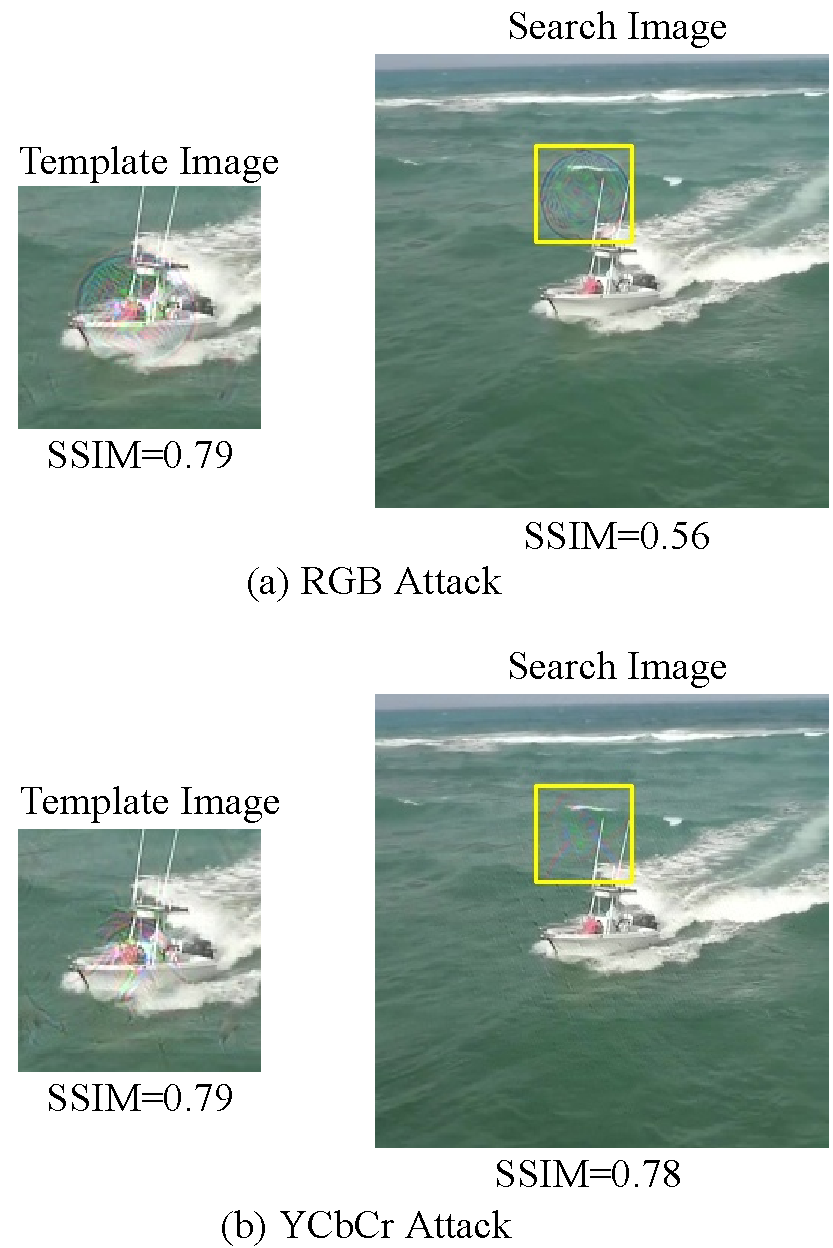
\includegraphics[width=0.48\textwidth]{images_imperceptible/1.pdf}
  \caption{\uline{Visualization of the perturbations.
  % 介绍什么是 RGB Attack
  Figure (a) demonstrates the pereturbations trained by the RGB attack method, i.e., the attack attack method proposed in Section III.
  % 介绍什么是 YCbCr Attack
  Figure (b) demonstrates the perturbations trained by the YCbCr attack method: first we convert the search image into YCbCr color space, then add pereturbations over the entire search image in the Y channel, and add perturbations over a very small region of $64 \times 64$ in the CbCr channel. 
  For the template image, we convert it into YCbCr color space, then add the perturbation over the entire template image in all YCbCr channels.
  The perturbed template and search images are then converted into RGB color scpace and fed into the tracking network.
  The other steps of the training process are the same as the attack method in Section III.
  Attacking the YCbCr color space brings better imperceptibility. Compared with attacking the RGB space, the SSIM of $p$ increases from 0.56 to 0.78. The SSIM of $\delta$ remains unchanged at 0.79.}
  }
  \label{fig:YCbCr}
\end{figure}

\begin{table}[t]
  \centering
  \caption{State-of-the-art comparison of untargeted attack performance on OTB2015 in terms of precision score.}
  \begin{tabular}{@{}rrccc@{}}
  \toprule
  \multirow{2}{*}[-1pt]{Method} & \multirow{2}{*}[-1pt]{Tracker} & \multirow{2}{*}[-1pt]{\begin{tabular}[c]{@{}c@{}}Attack Cost\\per Frame(ms)\end{tabular}} & \multirow{2}{*}[-1pt]{\begin{tabular}[c]{@{}c@{}}Before\\ Attack\end{tabular}} & \multirow{2}{*}[-1pt]{Untargeted Attack} \\
   &  &  &  &     \\ \midrule
  RTAA & DaSiamRPN & - & 0.880 & 0.050\\
  SPARK & SiamRPN & 41.4 & 0.851 & 0.064\\
  CSA & SiamRPN & 9 & 0.851 & 0.458\\
  FAN & SiamFC & 10 & 0.720 & 0.180\\
  TTP & SiamRPN++ & 8 & 0.910 & 0.080 \\
  \midrule
  Ours & SiamFC++ & $\sim 0$ & 0.861 & 0.092\\ \bottomrule
  \end{tabular}
  \label{tab:SOTA}
\end{table}

\begin{table}[t]
  \centering
  \caption{State-of-the-art comparison of targeted attack performance on OTB2015 in terms of precision score.}
  \begin{tabular}{@{}rrc@{}}
  \toprule
  Method & Tracker &  Targeted Attack \\
  \midrule
  FAN & SiamFC  &0.420 \\
  TTP & SiamRPN++ &0.692 \\
  \midrule
  Ours & SiamFC++  &0.795 \\ \bottomrule
  \end{tabular}
  \label{tab:SOTA1}
\end{table}

\subsection{Transferability Analysis}

\uline{In this sub-section, we analyze the transferability of the proposed attack method. Specifically, the perterbations are trained on SiamFC++\_GoogleNet, then we directly apply the perturbations to other tracking networks including SiamFC++\_ShuffleNet, SiamFC++\_AlexNet, SiamPRN and SiamRPN++.}

\textit{Transferability to Different Backbones} We evaluate the transferability of our attacks when applying the perturbations to two more different backbones of SiamFC++, \ie, ShuffleNet \cite{ShuffleNet} and AlexNet \cite{AlexNet}.
The experimental results are shown in Table \ref{tab:backbone}. In the case of SiamFC++-AlexNet, the AO with respect to the \textit{real trajectory} drops from 0.72 to 0.496. 
%\uline{
Our perturbations also generalize well to SiamFC++-ShuffleNet, despite the customized components such as pointwise group convolution and channel shuffle operations in ShuffleNet.
%}

\textit{Transferability to Different Tracking Architectures} We evaluate the transferability of our attacks when applying the perturbations to two more state-of-the-art anchor-based trackers: AlexNet-based SiamRPN \cite{SiamRPN} and ResNet-based SiamRPN++ \cite{SiamRPN++} to verify the transferability to different tracking architectures.
SiamRPN uses an RPN network to perform location regression and target classification on the response maps. SiamRPN++ performs layer-wise and depth-wise aggregation to improve accuracy based on the effective training using the ResNet backbone. The experimental results are shown in Table \ref{tab:arch}. In the case of SiamRPN, the AO with respect to the \textit{real trajectory} drops from 0.666 to 0.483 and the performance of SiamRPN++ is decreased from 0.676 to 0.418.
%We further analyze the performance of our attack method with respect to 11 attributes in OTB-2015 \cite{OTB}. As suggested in OTB \cite{OTB}, the attributes consist of out-of-view (OV), occlusion (OCC), illumination variation (IV), out-of-plane rotation (OPR), scale variation (SV),deformation (DEF), low resolution (LR), fast motion (FM), background clutters (BC), motion blur (MB), and in-plane rotation (IPR). Figure \ref{fig:attr} illustrates the untargeted attack results of the aforementioned trackers under the 11 attributes. 
The results show good transferability of our attacks to different tracking architectures, even if the generated perturbations are applied to anchor-based trackers.

\begin{table*}[t]
  \centering
  %\renewcommand\tabcolsep{3.5pt} % 调整表格列间的长度
  %\footnotesize
  \caption{State-of-the-art comparison of untargeted attack performance on VOT2016/2018 in terms of accuracy, robustness and expected average overlap (EAO).}
  \begin{tabular}{rrrcccccc}
  \toprule
  \multirow{2}{*}[-2pt]{Dataset} & \multirow{2}{*}[-2pt]{Method} & \multirow{2}{*}[-2pt]{Tracker} & \multicolumn{3}{c}{Before Attack} & \multicolumn{3}{c}{Untargeted Attack} \\ \cmidrule{4-9}
                           &                         &                          & Accuracy   & Robustness  & EAO    & Accuracy    & Robustness    & EAO     \\ \midrule
  \multirow{2}{*}{VOT2016} & RTAA                    & DaSiamRPN                & 0.625      & 0.224       & 0.439  & 0.521       & 1.613         & 0.078   \\
                           & Ours                    & SiamFC++                 & 0.626      & 0.144       & 0.460  & 0.393       & 9.061         & 0.007   \\ \midrule
  \multirow{5}{*}{VOT2018} & RTAA                    & DaSiamRPN                & 0.585      & 0.272       & 0.380  & 0.536       & 1.447         & 0.097   \\
                           & FAN                     & SiamFC                   & 0.503      & 0.585       & 0.188  & 0.420       & -             & -       \\
                           & CSA                     & SiamRPN                  & 0.570      & 0.440       & 0.261  & 0.430       & 1.900         & 0.076   \\
                           & TTP                     & SiamRPN++                & 0.600      & 0.320       & 0.340  & 0.520       & 7.820         & 0.014   \\
                           & Ours                    & SiamFC++                 & 0.587      & 0.183       & 0.426  & 0.342       & 8.981         & 0.007   \\ \bottomrule
  \end{tabular}
  \label{tab:sota_vot}
\end{table*}

\subsection{Comparison with Other Methods}

% \begin{figure}[t]
%   \begin{center}
%     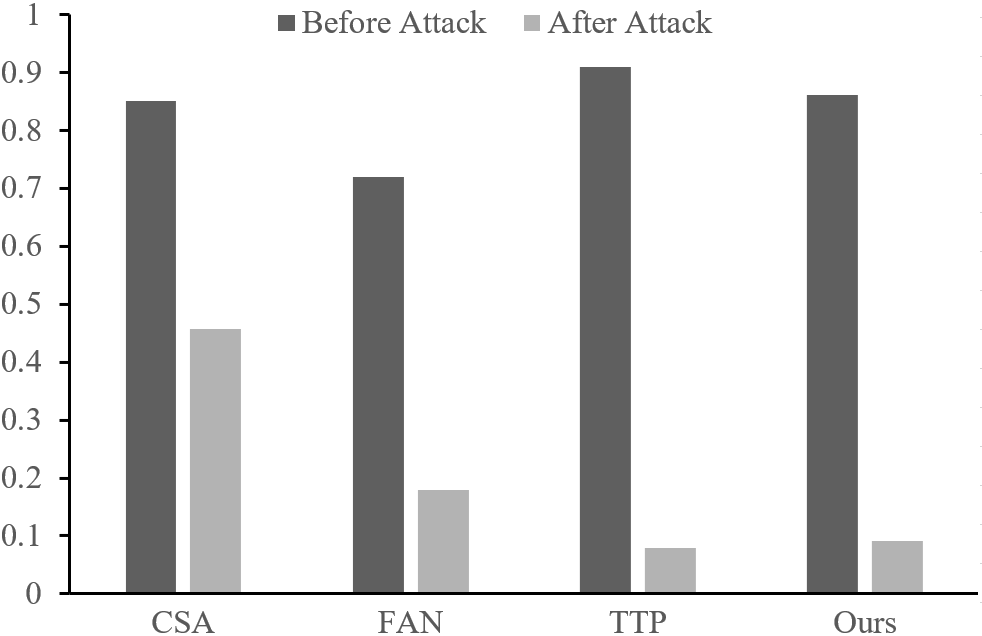
\includegraphics[width=0.48\textwidth]{images_imperceptible/SOTA.png}
%   \end{center}
%   \caption{Precision score with respect to the \textit{real trajectory} on OTB2015.}
%   \label{fig:SOTA}
% \end{figure}

\textit{OTB2015 Dataset} We compare the attack method proposed in this paper with the latest attack methods, including CSA \cite{CSA}, RTAA \cite{RTAA}, SPARK \cite{SPARK}, FAN \cite{FAN} and TTP \cite{TTP}. We report the untargeted attack result (Table \ref{tab:SOTA}) and the targeted attack result (Table \ref{tab:SOTA1}) on OTB2015.
SPARK \cite{SPARK} reduces the accuracy score with respect to the real trajectory from 0.851 to 0.064. However, SPARK needs to generate distinct adversarial examples for every search image through heavy iterative schemes, which is time-consuming to attack online-tracking in real time.
RTAA \cite{RTAA} reduces the accuracy score with respect to the real trajectory from 0.880 to 0.050. However, RTAA only performs the untargeted attacks for trackers, which is less challenging than the targeted attacks in this paper, as we aim to create arbitrary, complex trajectories at test time. 
Recently, Liang et al. proposed a fast attack network (FAN) \cite{FAN} for attacking SiamFC trackers. To perform untargeted attacks, FAN proposes a drift loss that shifts the tracker's prediction of the target's position. The tracking error accumulates over time until the tracker loses the target completely. To perform targeted attacks, FAN proposes embedding feature loss for improving the similarity between the features of the adversarial sample and the features of regions specified by a particular trajectory. FAN can reduce the accuracy score with respect to the real trajectory from 0.720 to 0.180. However, the accuracy score with respect to fake trajectories is only 0.420. Similar to SCA, FAN also requires running a generative network for each frame to obtain adversarial information. Nakka et al. \cite{TTP} proposed the temporally transferable perturbations (TTP) for attacking the SiamRPN++ tracker. TTP generates a single adversarial perturbation from the template image and adds this perturbation to each search image of the video. TTP reduces the accuracy score with respect to the real trajectory from 0.910 to 0.080, which is effective for untargeted attacks. However, the accuracy score with respect to the fake trajectory is only 0.692, which demonstrates that TTP's performance of targeted attacks is limited. In addition, this method needs to run a generative network for each video to obtain adversarial information, thus requires the computational and storage resources of the object tracking platform, which makes it difficult to deploy the method to resource-constrained platforms. Our method can reduce the accuracy score with respect to real trajectories from 0.861 to 0.092. The accuracy score is up to 0.795 with respect to fake trajectories, which is significantly better than other methods, and only needs to perform the add operation to generate adversarial information for any video without gradient optimization or network inference.

%\uline{
\textit{VOT2016/2018 Dataset} We compare the untargeted attack result with CSA \cite{CSA}, RTAA \cite{RTAA}, FAN \cite{FAN} and TTP \cite{TTP} on VOT2016 and VOT2018 (Table \ref{tab:sota_vot}). 
RTAA reduces the accuracy with respect to the real trajectory from 0.625 to 0.521 on VOT2016.
CSA \cite{CSA} is a Siamese tracking attack method called cooling-shrinking attack. CSA can suppress the peak region on the heat map reflecting the target location, which is used to attack the tracker's targeting ability. CSA can also simultaneously force the tracker's predicted bounding box to shrink, which is used to attack the bounding box regression capability of the tracker. However, this method requires running a generative network for each frame to obtain adversarial information, making it difficult to meet the demand for real-time tracking. CSA reduces the EAO with respect to the real trajectory from 0.261 to 0.076 on VOT2018. Compared to CSA, our method can achieve better untargeted attack results on VOT2018 with an EAO of 0.007.
%}

\uline{In summary, compared with other attack methods, our method has two key advantages. First, the proposed attack method does not require gradient optimization or network inference, making it possible to attack a real-world online-tracking system when we can not get access to the limited computational resources. Second, the proposed perturbations show good transferability to other anchor free or anchor based trackers. The main limitation of our work is the values of our universal perturbations are not as small as other non-universal perturbations due to the task difficulty.}

% 结论
\section{Conclusion}

In this paper, we propose a video-agnostic targeted attack method for Siamese trackers. 
We aim to attack the tracker by adding a perturbation to the template image and adding a \textit{fake target}, \ie, a small adversarial patch, into the search image adhering to the predefined trajectory, so that the tracker outputs the location and size of the \textit{fake target} instead of the real target. Being universal, the generated perturbations can be conveniently exploited to perturb videos on-the-fly without extra computations.
Experiments on several popular datasets show that our method can effectively fool the Siamese trackers in a targeted attack manner.
\uline{In future work, we expect that it will be possible to demonstrate the existence of a single perturbation to attack multi vision tasks, including image classification, object detection and video object tracking/segementation.}
% By studying the attack method of Siamese trackers, we argue that the disadvantage of Siamese trackers is that template matching-based tracking mechanism is vulnerable to attacks, i.e., if both the template and the search image are perturbed at the same time, then the tracking algorithm can easily be misled.
% The implication for improving the tracking robustness is to make the tracker aware of the semantic information of the target being tracked, rather than relying on templates alone, so that the semantic information can be relied on to ensure tracking robustness.

% 引文
\normalem
\bibliographystyle{IEEEtran}
\bibliography{ref}

% 作者
%\vfill  % 距离更远了
%\enlargethispage{-5in}  % 距离近了些
%\begin{IEEEbiography}[{
\includegraphics[width=1in,height=1.25in,clip,keepaspectratio]{images/zhbli.jpg}}]
\begin{IEEEbiography}[{
\includegraphics[width=1in,height=1.25in,clip]{images_imperceptible/author/zhbli.jpg}}]
{Zhenbang Li}
received the B.S. degree in computer science and technology from Beijing Institute of Technology, Beijing, China, in 2016. Currently, he is a Ph.D. student with the Institute of Automation, Chinese Academy of Sciences, Beijing, China. His research interests include object tracking and deep learning.
\end{IEEEbiography}

\begin{IEEEbiography}[{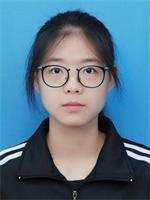
\includegraphics[width=1in,height=1.25in,clip]{images_imperceptible/author/yyshi.png}}]
  {YaYa Shi}
  received the B.S. degree from the Hefei University of Technology, Anhui, China in 2018. Currently, She is a Ph.D. student with the University of Science and Technology of China, Anhui, China. Her research interests include video captioning and deep learning.
\end{IEEEbiography}

\begin{IEEEbiography}[{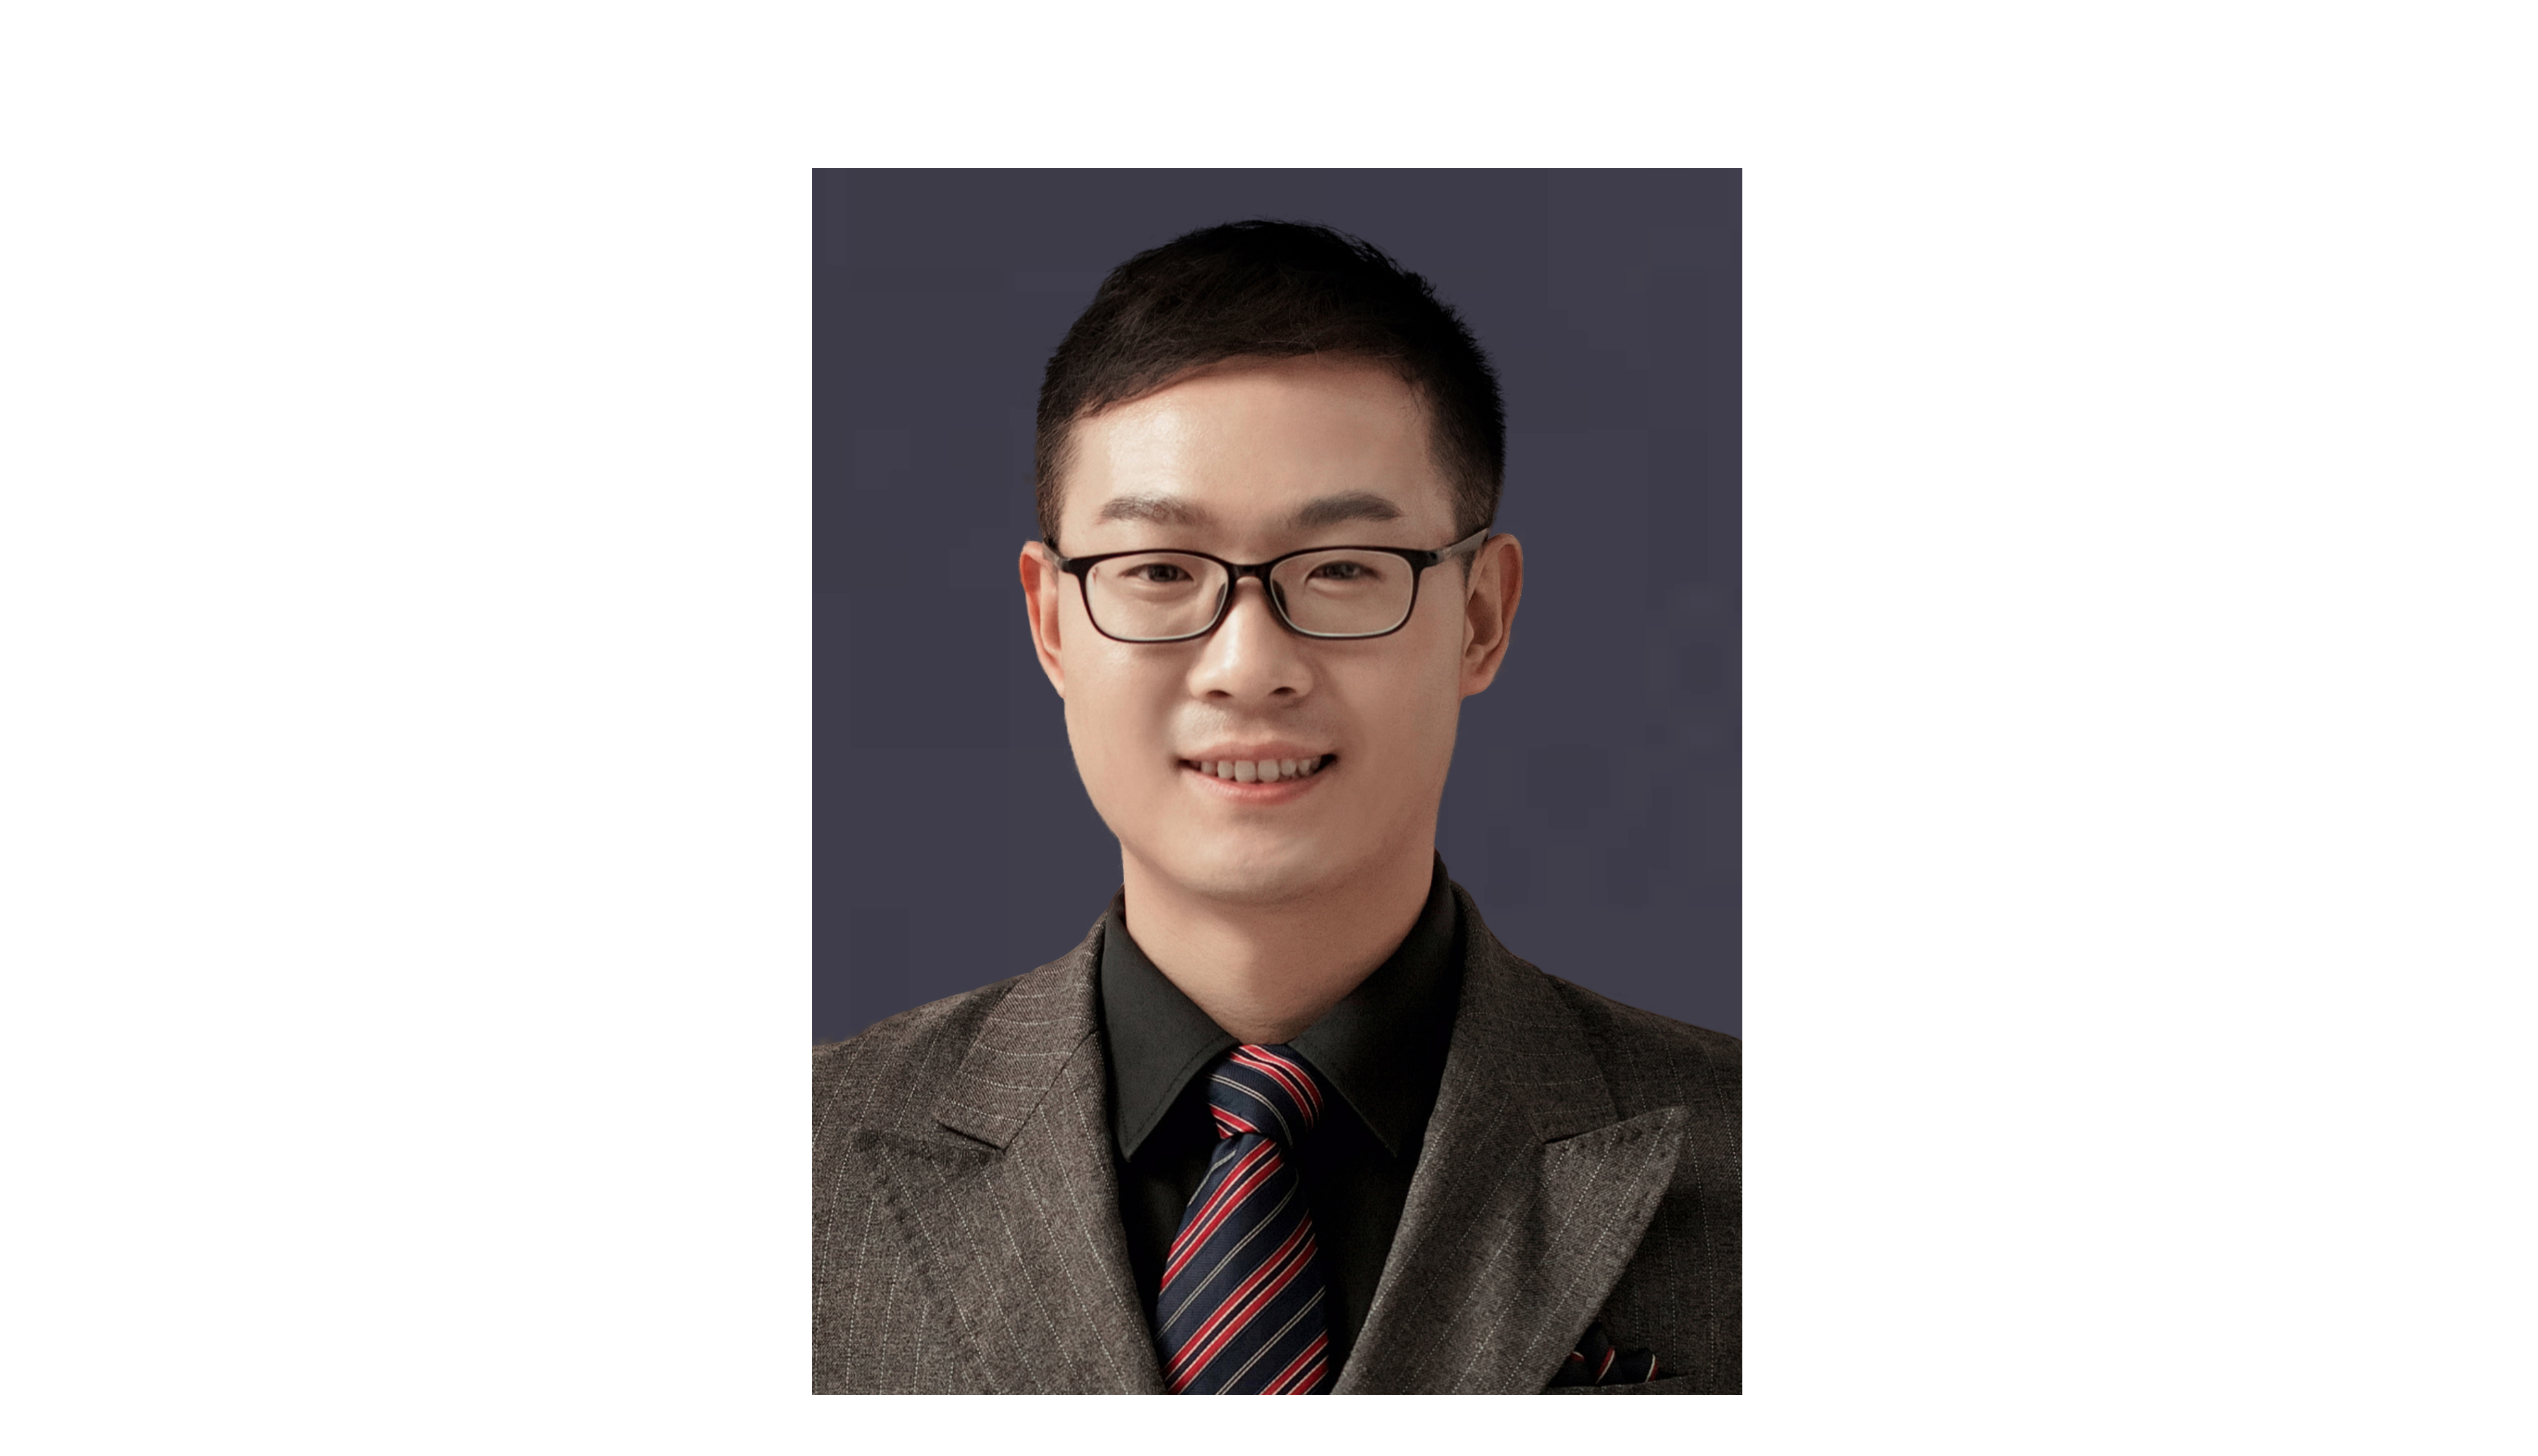
\includegraphics[width=1in,height=1.25in,clip]{images_imperceptible/author/JGao.pdf}}]
{Jin Gao}
received the B.S. degree from the Beihang University, Beijing, China, in 2010, and the Ph.D. degree from the University of Chinese Academy of Sciences (UCAS), in 2015. Now he is an associate professor with the National Laboratory of Pattern Recognition (NLPR), Institute of Automation, Chinese Academy of Sciences (CASIA). His research interests include visual tracking, autonomous vehicles, and service robots.
\end{IEEEbiography}

\begin{IEEEbiography}[{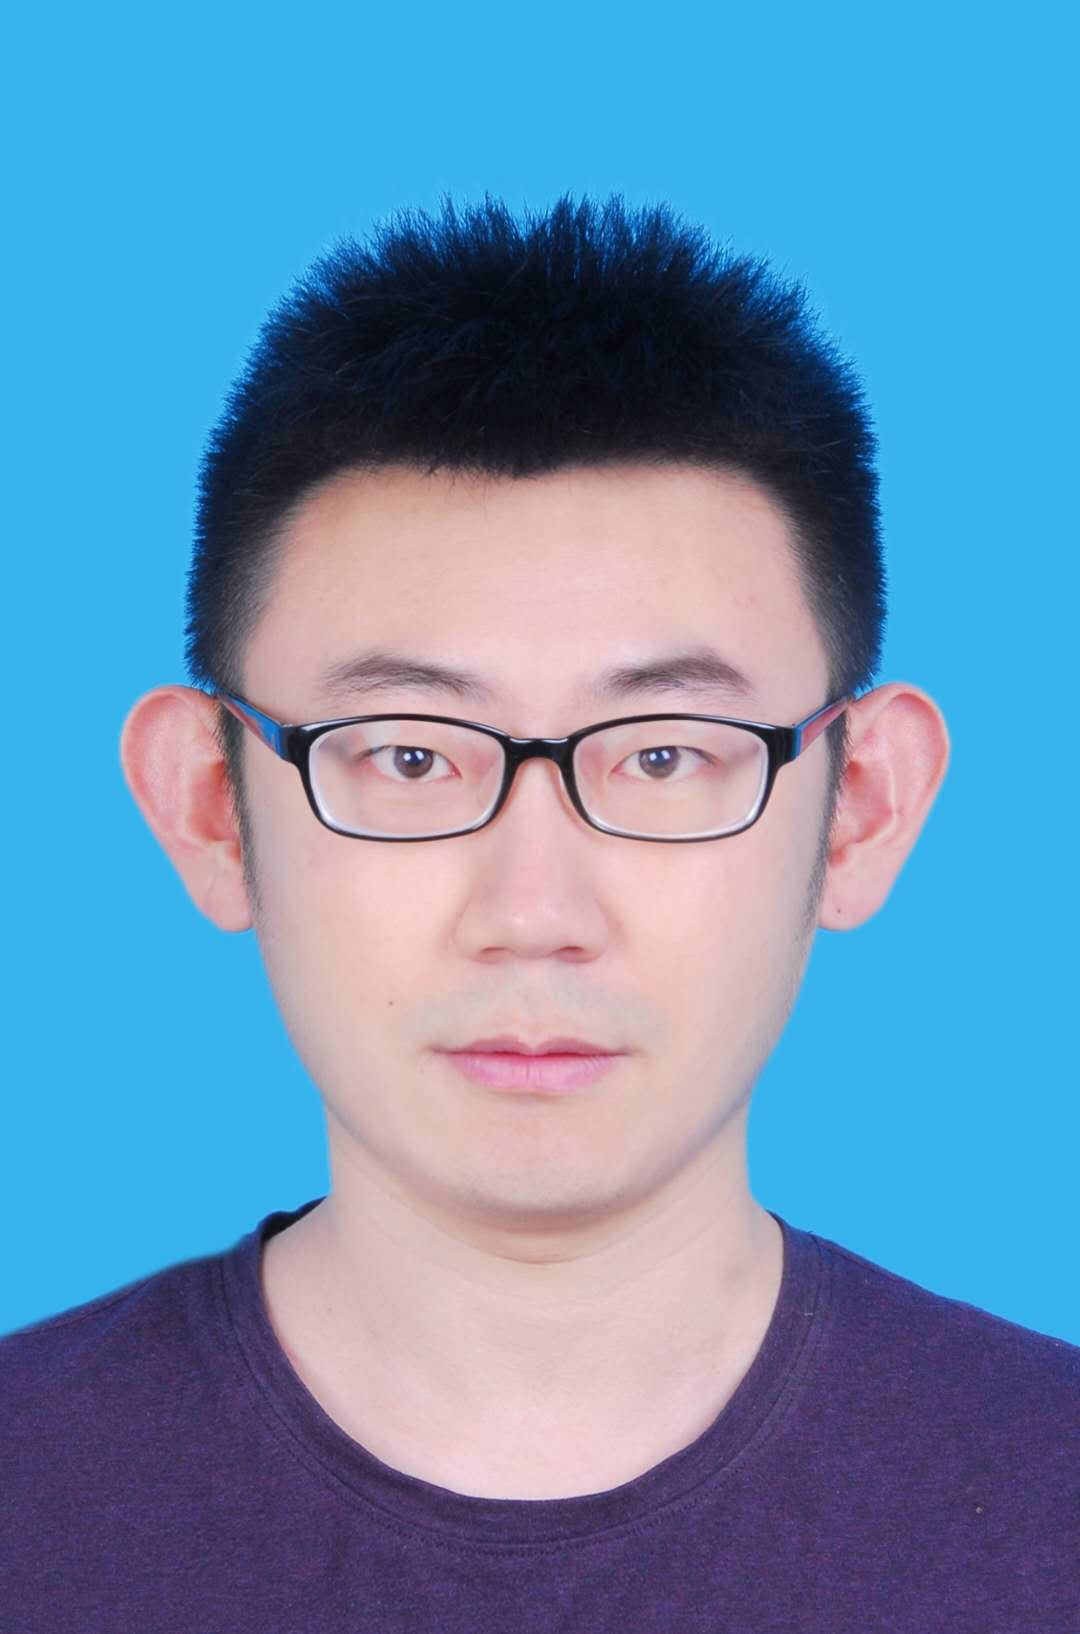
\includegraphics[width=1in,height=1.25in,clip]{images_imperceptible/author/srwang.jpg}}]
{Shaoru Wang}
received the B.E. degree from the Department of School of Information and Communication Engineering in Beijing University of Posts and Telecommunications, Beijing, China in 2018. He is currently pursuing his Ph.D. degree at the Institute of Automation, Chinese Academy of Sciences (CASIA), Beijing, China. His current research interests include computer vision and deep learning.
\end{IEEEbiography}

\begin{IEEEbiography}[{
\includegraphics[width=1in,height=1.25in,clip]{images_imperceptible/author/bli.pdf}}]
{Bing Li}
received the Ph.D. degree from the Department of Computer Science and Engineering, Beijing Jiaotong University, Beijing, China, in 2009. From 2009 to 2011, he worked as a Postdoctoral Research Fellow with the National Laboratory of Pattern Recognition, Institute of Automation, Chinese Academy of Sciences (CASIA), Beijing. He is currently a Professor with CASIA. His current research interests include computer vision, color constancy, visual saliency detection, multi-instance learning, and data mining.
\end{IEEEbiography}

\begin{IEEEbiography}[{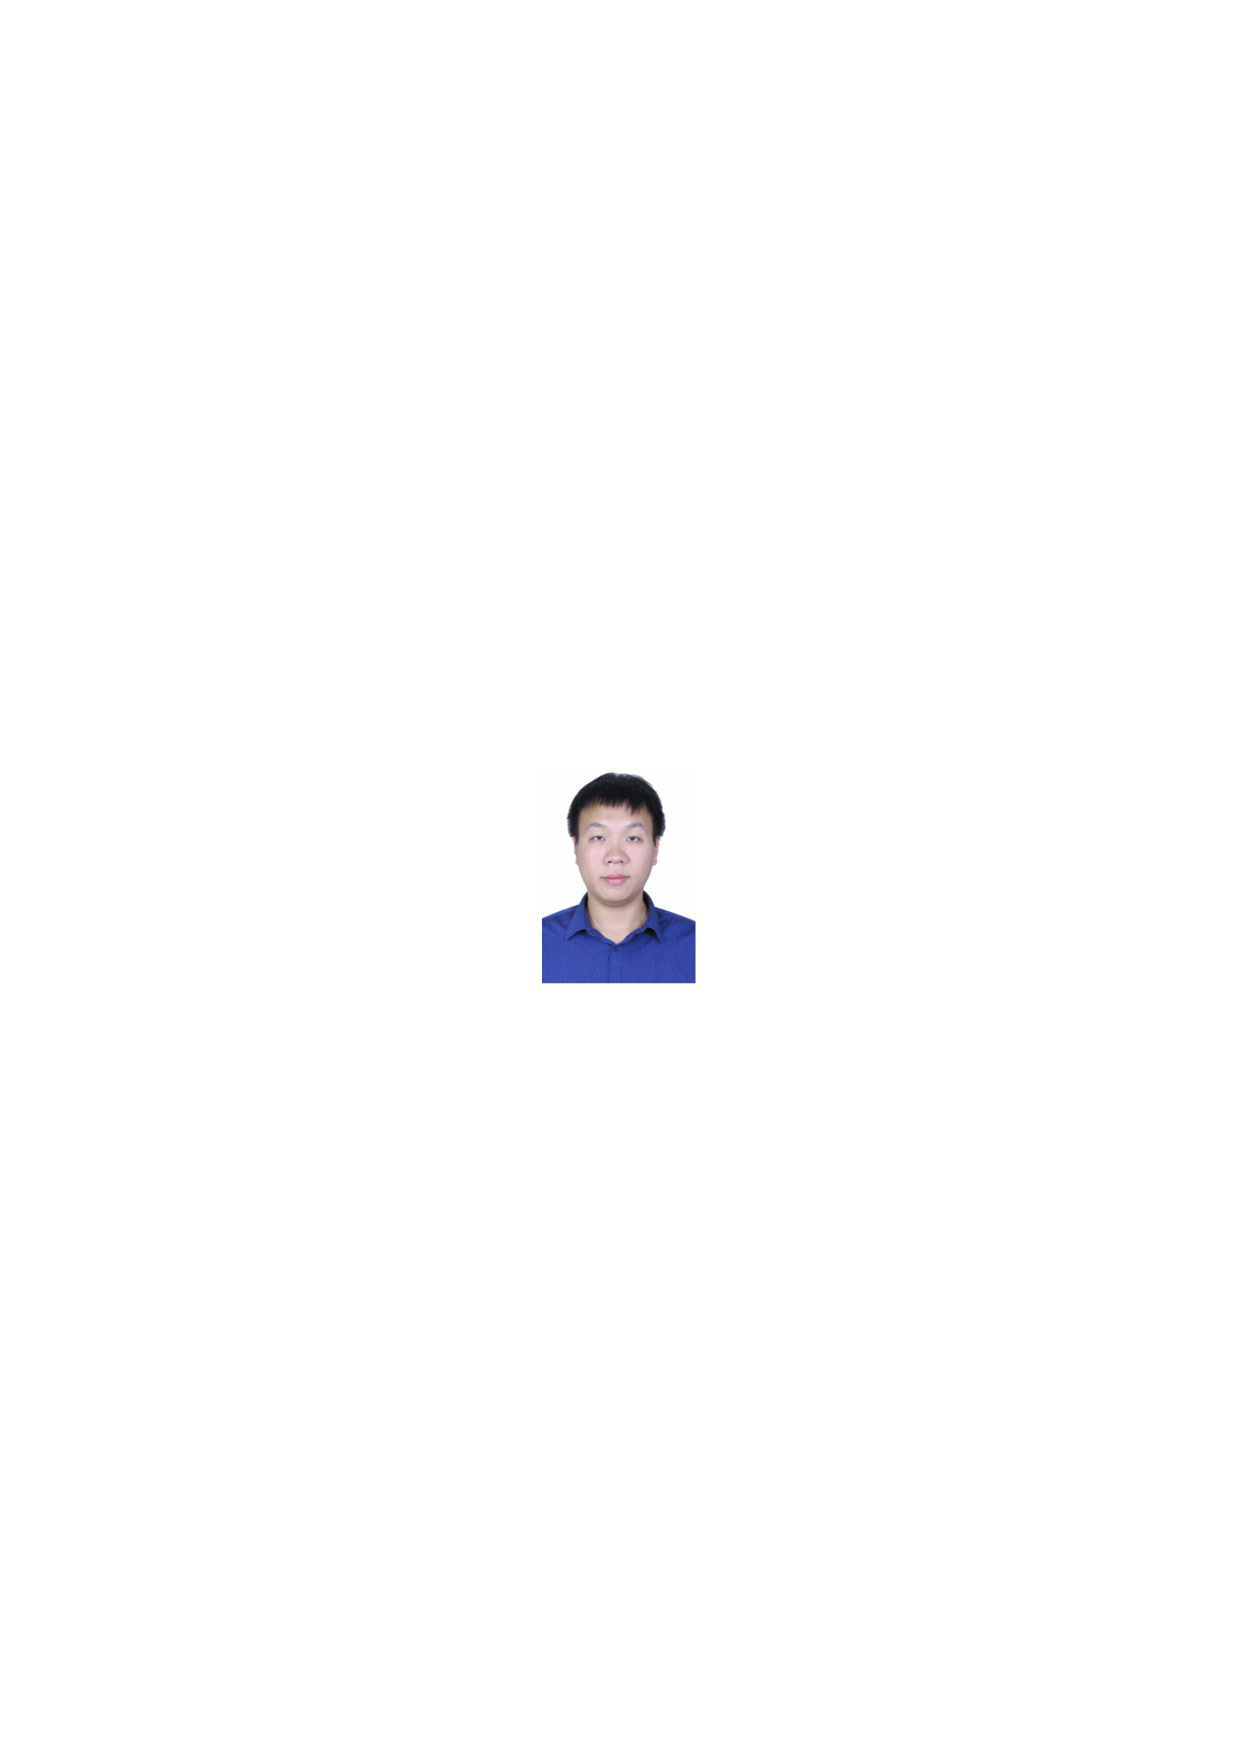
\includegraphics[width=1in,height=1.25in,clip]{images_imperceptible/author/Pengpeng-Liang.pdf}}]
{Pengpeng Liang}
received the B.S. and M.S. degrees in computer science from Zhengzhou University, China in 2008 and 2011, respectively and the Ph.D. degree from Temple University in 2016. He worked at Amazon from 2016 to 2017. Then, he joined Zhengzhou University as an assistant professor in the School of Information Engineering. His research interests include computer vision and deep learning.
\end{IEEEbiography}

\begin{IEEEbiography}[{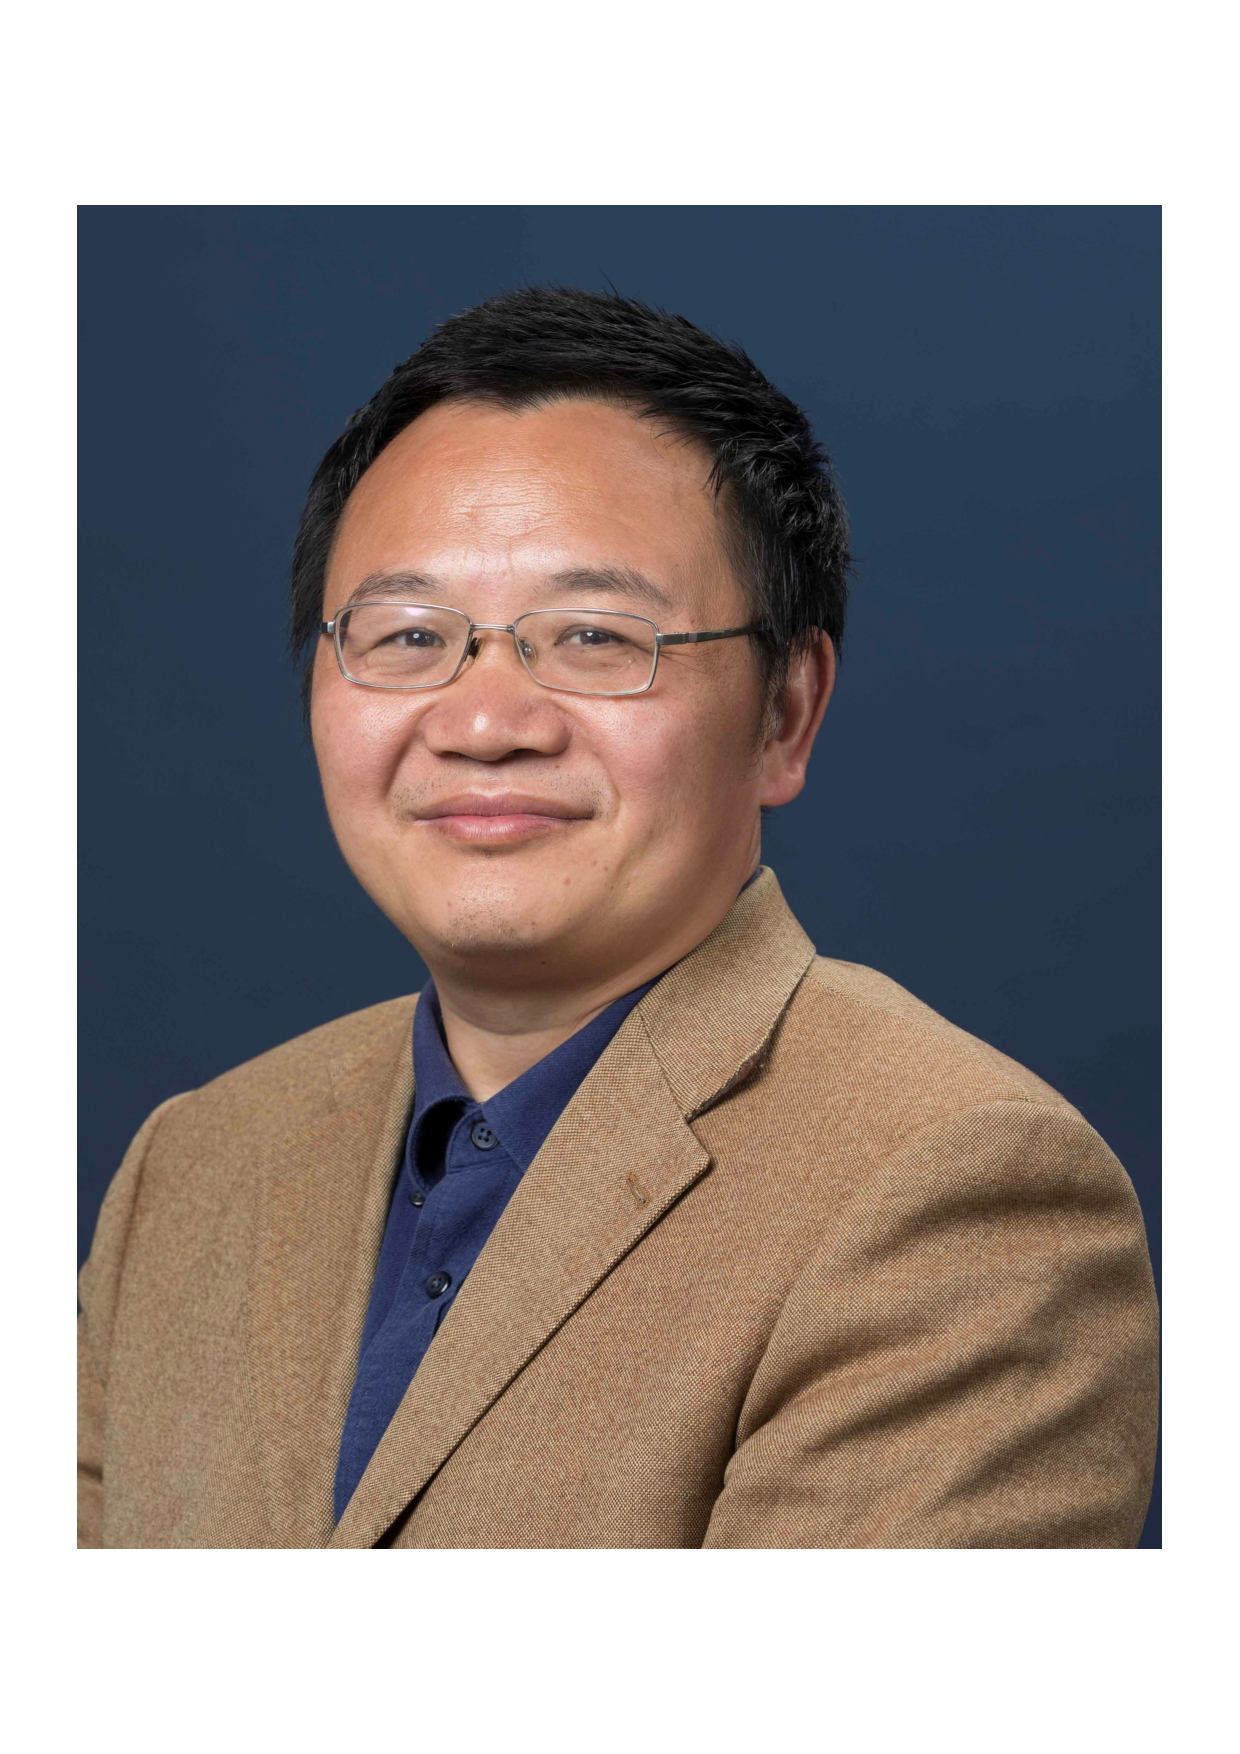
\includegraphics[width=1in,height=1.25in,clip]{images_imperceptible/author/wmhu.pdf}}]
{Weiming Hu}
received the Ph.D. degree from the Department of Computer Science and Engineering, Zhejiang University, Zhejiang, China. Since 1998, he has been with the Institute of Automation, Chinese Academy of Sciences (CASIA), Beijing, where he is currently a Professor. He has published more than 200 papers on peer reviewed international conferences and journals. His current research interests include visual motion analysis and recognition of harmful Internet multimedia.
\end{IEEEbiography}

\end{document}


